\documentclass[]{article}
\usepackage{lmodern}
\usepackage{amssymb,amsmath}
\usepackage{ifxetex,ifluatex}
\usepackage{fixltx2e} % provides \textsubscript
\ifnum 0\ifxetex 1\fi\ifluatex 1\fi=0 % if pdftex
  \usepackage[T1]{fontenc}
  \usepackage[utf8]{inputenc}
\else % if luatex or xelatex
  \ifxetex
    \usepackage{mathspec}
  \else
    \usepackage{fontspec}
  \fi
  \defaultfontfeatures{Ligatures=TeX,Scale=MatchLowercase}
\fi
% use upquote if available, for straight quotes in verbatim environments
\IfFileExists{upquote.sty}{\usepackage{upquote}}{}
% use microtype if available
\IfFileExists{microtype.sty}{%
\usepackage{microtype}
\UseMicrotypeSet[protrusion]{basicmath} % disable protrusion for tt fonts
}{}
\usepackage[margin=1in]{geometry}
\usepackage{hyperref}
\hypersetup{unicode=true,
            pdfborder={0 0 0},
            breaklinks=true}
\urlstyle{same}  % don't use monospace font for urls
\usepackage{color}
\usepackage{fancyvrb}
\newcommand{\VerbBar}{|}
\newcommand{\VERB}{\Verb[commandchars=\\\{\}]}
\DefineVerbatimEnvironment{Highlighting}{Verbatim}{commandchars=\\\{\}}
% Add ',fontsize=\small' for more characters per line
\usepackage{framed}
\definecolor{shadecolor}{RGB}{248,248,248}
\newenvironment{Shaded}{\begin{snugshade}}{\end{snugshade}}
\newcommand{\KeywordTok}[1]{\textcolor[rgb]{0.13,0.29,0.53}{\textbf{{#1}}}}
\newcommand{\DataTypeTok}[1]{\textcolor[rgb]{0.13,0.29,0.53}{{#1}}}
\newcommand{\DecValTok}[1]{\textcolor[rgb]{0.00,0.00,0.81}{{#1}}}
\newcommand{\BaseNTok}[1]{\textcolor[rgb]{0.00,0.00,0.81}{{#1}}}
\newcommand{\FloatTok}[1]{\textcolor[rgb]{0.00,0.00,0.81}{{#1}}}
\newcommand{\ConstantTok}[1]{\textcolor[rgb]{0.00,0.00,0.00}{{#1}}}
\newcommand{\CharTok}[1]{\textcolor[rgb]{0.31,0.60,0.02}{{#1}}}
\newcommand{\SpecialCharTok}[1]{\textcolor[rgb]{0.00,0.00,0.00}{{#1}}}
\newcommand{\StringTok}[1]{\textcolor[rgb]{0.31,0.60,0.02}{{#1}}}
\newcommand{\VerbatimStringTok}[1]{\textcolor[rgb]{0.31,0.60,0.02}{{#1}}}
\newcommand{\SpecialStringTok}[1]{\textcolor[rgb]{0.31,0.60,0.02}{{#1}}}
\newcommand{\ImportTok}[1]{{#1}}
\newcommand{\CommentTok}[1]{\textcolor[rgb]{0.56,0.35,0.01}{\textit{{#1}}}}
\newcommand{\DocumentationTok}[1]{\textcolor[rgb]{0.56,0.35,0.01}{\textbf{\textit{{#1}}}}}
\newcommand{\AnnotationTok}[1]{\textcolor[rgb]{0.56,0.35,0.01}{\textbf{\textit{{#1}}}}}
\newcommand{\CommentVarTok}[1]{\textcolor[rgb]{0.56,0.35,0.01}{\textbf{\textit{{#1}}}}}
\newcommand{\OtherTok}[1]{\textcolor[rgb]{0.56,0.35,0.01}{{#1}}}
\newcommand{\FunctionTok}[1]{\textcolor[rgb]{0.00,0.00,0.00}{{#1}}}
\newcommand{\VariableTok}[1]{\textcolor[rgb]{0.00,0.00,0.00}{{#1}}}
\newcommand{\ControlFlowTok}[1]{\textcolor[rgb]{0.13,0.29,0.53}{\textbf{{#1}}}}
\newcommand{\OperatorTok}[1]{\textcolor[rgb]{0.81,0.36,0.00}{\textbf{{#1}}}}
\newcommand{\BuiltInTok}[1]{{#1}}
\newcommand{\ExtensionTok}[1]{{#1}}
\newcommand{\PreprocessorTok}[1]{\textcolor[rgb]{0.56,0.35,0.01}{\textit{{#1}}}}
\newcommand{\AttributeTok}[1]{\textcolor[rgb]{0.77,0.63,0.00}{{#1}}}
\newcommand{\RegionMarkerTok}[1]{{#1}}
\newcommand{\InformationTok}[1]{\textcolor[rgb]{0.56,0.35,0.01}{\textbf{\textit{{#1}}}}}
\newcommand{\WarningTok}[1]{\textcolor[rgb]{0.56,0.35,0.01}{\textbf{\textit{{#1}}}}}
\newcommand{\AlertTok}[1]{\textcolor[rgb]{0.94,0.16,0.16}{{#1}}}
\newcommand{\ErrorTok}[1]{\textcolor[rgb]{0.64,0.00,0.00}{\textbf{{#1}}}}
\newcommand{\NormalTok}[1]{{#1}}
\usepackage{longtable,booktabs}
\usepackage{graphicx,grffile}
\makeatletter
\def\maxwidth{\ifdim\Gin@nat@width>\linewidth\linewidth\else\Gin@nat@width\fi}
\def\maxheight{\ifdim\Gin@nat@height>\textheight\textheight\else\Gin@nat@height\fi}
\makeatother
% Scale images if necessary, so that they will not overflow the page
% margins by default, and it is still possible to overwrite the defaults
% using explicit options in \includegraphics[width, height, ...]{}
\setkeys{Gin}{width=\maxwidth,height=\maxheight,keepaspectratio}
\IfFileExists{parskip.sty}{%
\usepackage{parskip}
}{% else
\setlength{\parindent}{0pt}
\setlength{\parskip}{6pt plus 2pt minus 1pt}
}
\setlength{\emergencystretch}{3em}  % prevent overfull lines
\providecommand{\tightlist}{%
  \setlength{\itemsep}{0pt}\setlength{\parskip}{0pt}}
\setcounter{secnumdepth}{0}
% Redefines (sub)paragraphs to behave more like sections
\ifx\paragraph\undefined\else
\let\oldparagraph\paragraph
\renewcommand{\paragraph}[1]{\oldparagraph{#1}\mbox{}}
\fi
\ifx\subparagraph\undefined\else
\let\oldsubparagraph\subparagraph
\renewcommand{\subparagraph}[1]{\oldsubparagraph{#1}\mbox{}}
\fi

%%% Use protect on footnotes to avoid problems with footnotes in titles
\let\rmarkdownfootnote\footnote%
\def\footnote{\protect\rmarkdownfootnote}

%%% Change title format to be more compact
\usepackage{titling}

% Create subtitle command for use in maketitle
\providecommand{\subtitle}[1]{
  \posttitle{
    \begin{center}\large#1\end{center}
    }
}

\setlength{\droptitle}{-2em}

  \title{}
    \pretitle{\vspace{\droptitle}}
  \posttitle{}
    \author{}
    \preauthor{}\postauthor{}
    \date{}
    \predate{}\postdate{}
  
\usepackage{booktabs}
\usepackage{longtable}
\usepackage{array}
\usepackage{multirow}
\usepackage{wrapfig}
\usepackage{float}
\usepackage{colortbl}
\usepackage{pdflscape}
\usepackage{tabu}
\usepackage{threeparttable}
\usepackage{threeparttablex}
\usepackage[normalem]{ulem}
\usepackage{makecell}
\usepackage{xcolor}

\usepackage{graphicx,latexsym}
\usepackage{amssymb,amsthm,amsmath}
\usepackage{longtable,booktabs,setspace}
\usepackage{lscape}

\begin{document}

\section{La familia PriA}\label{la-familia-pria}

\begin{figure}[h!tbp]
\centering
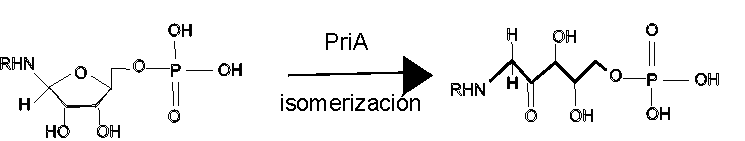
\includegraphics[angle = 0,scale = 1]{chapter4/isomerizacion.pdf}
\caption[La reacción que cataliza PriA es una isomerización donde abre un anillo de cinco carbonos.]{\footnotesize{La reacción que cataliza PriA es una isomerización donde abre un anillo de cinco carbonos.}}
\label{fig:isomerizacion}
\end{figure}

PriA es una familia de enzimas de Actinobacteria homóloga a la familia
HisA en Enterobacteria. Según las definiciones de este trabajo PriA es
una familia promiscua. Varios miembros de PriA han sido sujetos a
estudios de cinéticas enzimáticas demostrándose su capacidad de
catalizar tanto la reacción correspondiente a HisA como la de TrpF. Es
decir PriA participa a la vez en las rutas de síntesis de Histidina y
Triptofano, al menos en varias Actinobacterias. Los primeros miembros
caracterizados como promiscuos en esta familia en el 2003 fueron
\emph{Streptomyces coelicolor} y \emph{Mycobacterium tuberculosis}
{[}@baronagomez\_occurrence\_2003{]}. La mayoría de las actinobacterias
han perdido el gen trpF en la ruta del triptofano, por lo que se cree
que la promiscuidad de PriA está extendida en un gran subconjunto de
Actinobacteria. PriA en la ruta de histidina isomeriza el sustrato
ProFAR en PRFAR, realizando la función HisA. En la ruta de triptofano
lleva a cabo la isomerización de PRA en CdRP actuando análogamente a la
función TrpF en la ruta del triptófano. En \emph{Streptomyces
coelicolor} varios genes de los operones de histidina y triprofano están
en la vecindad genómica de PriA.

Además, en Actinobacteria PriA ha mostrado un gradiente funcional. Esta
variación divide a la familia en varias subfamilias según su capacidad
catalíticas en los sustratos ProFAR y PRA. En la \autoref{tab:cineticos}
se muestra la constantes catalíticas de PriA estimadas en diferentes
organismos para estos dos sustratos. Estos datos ejemplifican las
subfamilias de PriA, en la tabla se encuentran ejemplos de miembros de
PriB, la subfamilia ubicada en el género \emph{Streptomyces} con baja
capacidad de catálisis para la función TrpF. Varios \emph{Streptomyces}
con un ortólogo en la familia PriB, se diferencian de otras
Actinobacterias en que contienen en su genoma un gen \emph{trpF}
localizado fuera del contexto genómico inmediato de los operones de
histidina y triptofano. Otra subfamilia de PriA es subHisA, que ha
perdido totalmente la actividd TrpF, existen miembros de subHisA en
\emph{Corynebacteria} y en \emph{Actinomyces}. Finalmente en Actinomyces
encontramos la subfamilia \emph{subTrpF} que ha perdido la actividad de
HisA.

En este capítulo en las siguientes secciones se exploran cuatro apectos
de la familia PriA. \emph{i)} La distribución y el contexto genómico de
PriA en diversos linajes genómicos. \emph{ii)} La información contenida
a nivel de aminoácidos en variantes de PriA como medio de studio de
rutas evolutivas y su relación con la reconstrucción de su estructura
tridimensional. \emph{iii)} Las posibles afinidades de PriA por otros
sustratos con métodos bioinformáticos, y finalmente \emph{iv)} La
validación experimental de PriA en sustratos diferentes de PRA y ProFAR
o bien en combinaciones de los mismos.

\begin{longtable}[]{@{}l@{}}
\caption{Reclutamientos de expansiones de PriA en MIBiG
\label{tab:cineticos}}\tabularnewline
\toprule
--------------------------------------------------------------------------\tabularnewline
\bottomrule
\end{longtable}

\clearpage    

\textbackslash{}begin\{landscape\}

\$\$ \resizebox{\columnwidth}{!}{%
\begin{tabular}{ l c r c c c c c c c l}
\hline \\ [-1.5ex]
Fuente  &Familia & HisA $in\hspace{.1cm}vivo$ &TrpF $in\hspace{.1cm}vivo$ & $K{cat}^{ProFAR}[M^{-1}s^{-1}]$ & $Km^{ProFAR}[\mu M]$& $\frac{K{cat}}{Km} ProFAR$ & $K{cat}^{PRA}[M^{-1}s^{-1}]$ & $Km^{PRA}[\mu M]$  &  $\frac{Kcat}{Km} PRA $  &Referencia  \\ [1ex]
\hline \\ [-1.5ex]  
\textit{Escherichia} \textit{coli}         & HisA &- &- & 1.6 & 4.9 & 3.1 & -   & -   & 0   & Henn-Sax 2002 \\ [1ex]  
\textit{Escherichia}  \textit{coli}        &TrpF  &- &- &-    &-    &0    & 12.2& 34.5& 2.82& Sterner 1996 \\ [1ex]    
\textit{Mycobacterium} \textit{tuberculosis} &PriA&-&-&19&0.23&12&21&3.6&0.17& Due 2011\\ [1ex]    
\textit{Mycobacterium}  \textit{smegmatis} &PriA&*&*& 2.6 ± 0.5 & 0.85 $ \pm $ 0.04 &0.33& 7.9 $ \pm $  2.4& 3.1 $ \pm $0.43  &0.39& Verduzco-Castro 2016 \\ [1ex]   
\textit{Streptomyces} \textit{globisporus}  &PriA&*&*& 4.2 ± 0.8& 0.74 ± 0.03 &0.18& 11 ± 1.0 & 3.8 ± 0.2 &0.34& Verduzco-Castro 2016\\ [1ex]  
\textit{Streptomyces} \textit{coelicolor} &PriA&-&-& 3.6 ± 0.7 & 1.3 ± 0.2 &0.4& 5.0 ± 0.08 & 3.4 ± 0.09 &0.7& Noda-Garcia 2010\\ [1ex]   
\textit{Streptomyces} \textit{ipomoeae}  &PriB&*&*& 3.8 ± 0.2 & 0.82 ± 0.02 &0.21& 60.8 ± 1.1&  8.25 ± 0.4&0.14& Verduzco-Castro 2016\\ [1ex]   
\textit{Streptomyces} sp. Mg1  &PriB&*&*& 13.2 ± 3.4 &0.92 ± 0.19 &69&129.6 ± 34 &0.29 ± 0.04&0.0022&Verduzco-Castro 2016\\ [1ex]  
\textit{Streptomyces} sp. C&PriB&*&*&11.4 ± 3.4 &2.53 ± 0.74 &0.22&149. 9 ± 29& 1.4 ± 0.12 &9&Verduzco-Castro 2016\\ [1ex]    
\textit{Streptomyces} \textit{sviceus} &PriB&*&*&3.9 ± 0.89 &0.69 ± 0.04 &0.18&24.5 ± 4.0& 1.6 ± 0.29 &67&VVerduzco-Castro 2016\\ [1ex]   
\textit{Corynebacterium} \textit{diphteriae} &subHisA&-&-&4.4 ± 0.5&2.6 ± 0.3&0.59&&&0& Noda-Garcia 2013\\ [1ex]    
\textit{Corynebacterium} \textit{jeikeium} &PriA&-&-&2.3 ± 0.2&0.9 ± 0.08&0.39&5.1 ± 1.0&1.6 ± 0.16&0.31& Noda-Garcia 2013\\ [1ex]    
\textit{Corynebacterium} \textit{striatum} &subHisA&-&-&6.9 ± 0.7&2.1 ± 0.5&0.3&&&0& Noda-Garcia 2013 \\ [1ex]    
\textit{Corynebacterium} \textit{diphteriae}  L48I-F50L-T80S&subHisA&&&4.5 ± 1.5&0.6 ± 0.08&0.13&133 ± 10&0.05 ± 0.01&0.0004&NNoda-Garcia 2013\\ [1ex]    
\textit{Actinomyces} \textit{urogenitalis} DSM 15434&PriB&*&*&2.1 ± 0.5 &1.8 ± 0.2 &0.9&26.3 ± 6.3& 0.37 ± 0.09 &14&Verduzco-Castro 2016\\ [1ex]   
\textit{Actinomyces} \textit{odontolyticus}  ATCC 17982&subTrpF&&*&-&-&0&&&0.02&Juarez-Vazquez 2017\\ [1ex]    
\textit{Actinomyces} \textit{oris} K20 BABV01&PriA&&&&&0.02&&&0.01&Juarez-Vazquez 2017\\ [1ex]    
\textit{Actinomyces} sp. oral taxon 171 str. F0337&PriA&&&&&0.01&&&4&Juarez-Vazquez 2017\\ [1ex]    
\textit{Actinomyces} sp. oral taxon 848 str. F0332&subTrpF&&*&-&-&0&&&0.0001&Juarez-Vazquez 2017\\ [1ex]    
\textit{Actinomyces} \textit{urogenitalis} DSM 15434&PriA&&&&&0.01&&&0.02&Juarez-Vazquez 2017\\ [1ex]    
\textit{Bifidobacterium} \textit{adolescentis} L2-32&PriA&*&*&&&0.2&&&0.1&Juarez-Vazquez 2017\\ [1ex]    
\textit{Bifidobacterium} \textit{gallicum} DSM 20093 &PriA&*&*&&&0.1&&&0.04&Juarez-Vazquez 2017\\ [1ex]    
\textit{Bifidobacterium} \textit{longum} ATCC 15697&PriA&*&*&&&0.1&&&0.3&Juarez-Vazquez 2017\\ [1ex]    
Camera CAM1&Metagenoma&&&1.7 ± 0.1&0.3 ± 0.03&0.2&40 ± 7&3.5 ± 0.04&0.09&Noda-Garcia 2015\\ [1ex]    
CAM1 A81G&Metagenoma&&&1.7 ± 0.2&0.1 ± 0.01&0.06&32.2 ± 1.7&1.9 ± 0.1&0.06&Noda-Garcia 2015\\ [1ex]    
CAM1 A81S&Metagenoma&&&4.0 ± 0.9&0.2 ± 0.03&0.04&23.5 ± 6.5&0.5 ± 0.1&0.02&Noda-Garcia 2015\\ [1ex]    
CAM2&Metagenoma&&&n.d.&n.d.&0&n.d.&n.d.&0&Noda-Garcia 2015\\ [1ex]    
PriA Ancestral&Ancestral&&&9.4±1.6&0.3±0.009&0.03&4.3±0.4&0.6±0.02&0.13&Verduzco, Noda, sin publicar\\ [1ex]    
PriA SubHisA&Ancestral&&&3.7±1.01&0.5±0.03&0.1&-&-&0&Verduzco, Noda, sin publicar\\ [1ex]    
SubHisA Ancestral&Ancestral&&&6.3±0.7&0.15±0.03&0.02&-&-&0&Verduzco, Noda, sin publicar\\ [1ex]    
SubHisA PriA&Ancestral&&&27.7±3.4&0.05±0.005&2&167.82&0.03±0.002&0.0001&Verduzco, Noda, sin publicar\\ [1ex]    
\textit{Streptomyces} \textit{acidiscabies}&&0&0&163.6&0.1&&&&&Verduzco*\\ [1ex]  
\textit{A} \textit{visco} &&&46&1.37&36&3.4&&&&Juárez*\\ [1ex]  

\hline \\ [-1.5ex]
\hline
\end{tabular}} \%\} \$\$

\textbackslash{}end\{landscape\} \normalsize

\subsection{PriA como modelo de familia enzimática donde las expansiones
no son condición necesaria para la
promiscuidad.}\label{pria-como-modelo-de-familia-enzimatica-donde-las-expansiones-no-son-condicion-necesaria-para-la-promiscuidad.}

\paragraph{PriA en EvoMining}\label{pria-en-evomining}

Para explorar PriA en diversos linajes genómicos se utilizaron las
herramientas EvoMining y CORASON descritas en los capítulos previos. Se
investigaron las expansiones de la familia PriA en los linajes
Actinobacteria, Cyanobacteria, \emph{Pseudomonas} y Archaea. En
Actinobacteria, donde se sabe que PriA es promiscua no se detectaron
copias extra. En la \autoref{fig:PriA_Expansiones} se muestra el número
promedio de copias por genoma en los linajes genómicos seleccionados.
Según EvoMining en Actinobacteria no hay expansiones, prácticamente
todas las copias son reconocidas como de metabolismo central (rojo o
morado) aunque algunas PriA además son marcadas por antiSMASH como parte
de algún cluster biosintético (morado). En cambio en Cyanobacteria,
\emph{Pseudomonas} y Archaea la figura muestra en negro las copias extra
de las que no se conoce su destino metabólico. El caso de Archaea es
llamativo porque las copias de metabolismo central llegan en promedio
hasta .5 copias por genoma, es decir muchos genomas de Archaea no
cuentan con una copia de PriA, y en cambio, contrario a Actinobacteria,
un 50\% de la copias es marcado en negro, es decir varios de los genomas
que tienen al menos una copia de PriA en realidad tienen dos copias.Esta
figura muestra que en Actinobacteria PriA consituye un ejemplo de
familia promiscua mayoritariamente distribuida con una sola copia por
genoma. Esta observación demuestra que para que una familia sea
promiscua no es imperativo tener copias extra con marcas de
reclutamiento en metabolismo especializado. Aunque las copias extra
suelen ser una indicación de promiscuidad, no son una condición
necesaria. Tanto EvoMining como CORASON mostraron que existen
excepciones de organismos donde PriA tiene doble copia, tanto en
Actinobacteria como en otros linajes genómicos.

\begin{figure}[h!tbp]
\centering
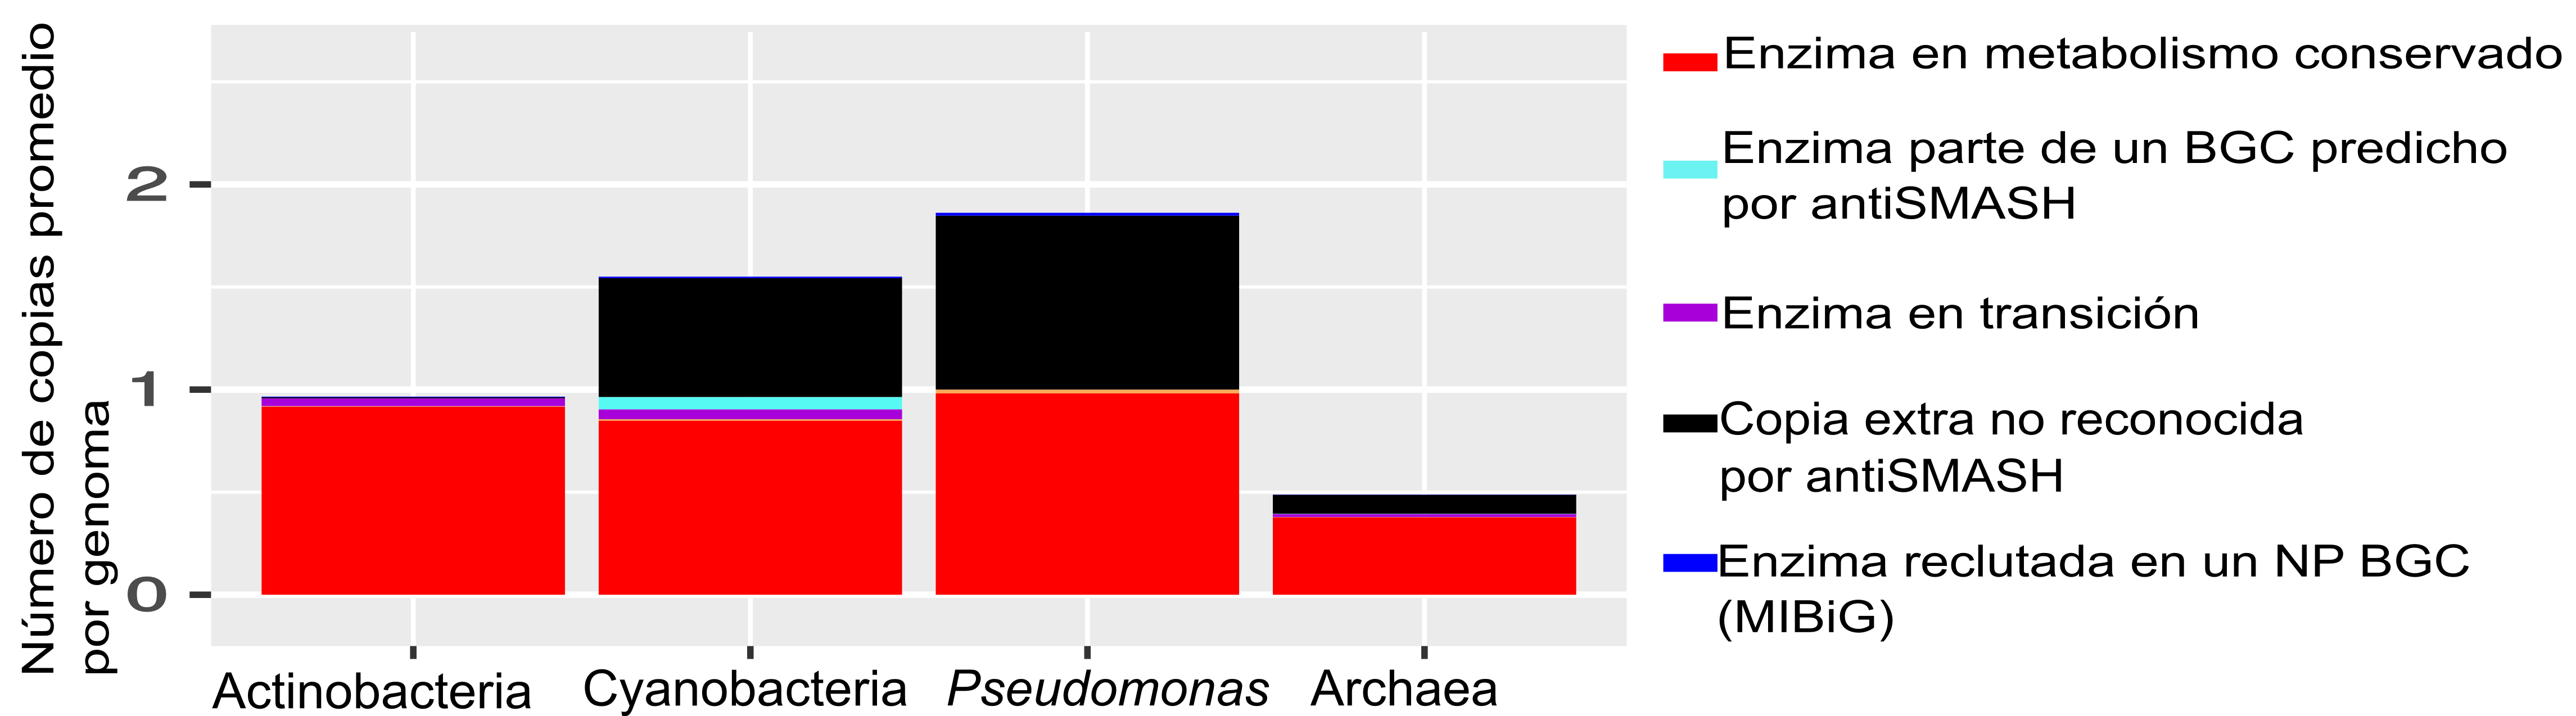
\includegraphics[angle = 0,scale = 0.8]{chapter4/PriAExpansiones.png}
\caption[Expansiones de PriA en Actinobacteria, Cyanobacteria, Pseudomonas y Archaea]{\footnotesize{Número promedio de copias por genoma de PriA en Actinobacteria, Cyanobacteria, Pseudomonas y Archaea. Los colores muestran el destino metabólico asignado a cada copia según EvoMining. En rojo están los BBH a las enzimas semilla de metabolismo central. En morado las enzimas de metabolismo central también reconocidas por antiSMASH como parte de unBGC y en negro las copias sin un destino metabólico conocido.}}
\label{fig:PriA_Expansiones}
\end{figure}

Después del conteo de número de copias promedio, se analizaron los
árboles de PriA de EvoMining, tanto los coloreados de acuerdo al número
de copias, \autoref{fig:PriAEvoMiningCopies}, como los coloreados según
el destino metabólico, \autoref{fig:PriATrees}. En Actinobacteria la
mayoría de las hojas son verdes reafirmando que existe sólo una copia
por genoma en ese organismo. Sin embargo, existen varias hojas de color
amarillo, indicando de dos copias en ese genoma. Las Actinobacterias con
dos copias son \emph{Ornithinimicrobium pekingense} DSM 21552,
\emph{Pseudonocardia} sp. P2, \emph{Serinicoccus marinus} DSM 15273,
\emph{Serinicoccus profundi} MCCC 1A05965, \emph{Sphaerobacter
thermophilus} DSM 20745 y \emph{Streptomyces} sp. CT34.

En Cyanobacteria, \emph{Pseudomonas} y Archaea en contraste con
Actinobacteria, se muestran una mezcla entre organismos que poseen una
(verdes) o dos copias (amarillos) de PriA. Sin embargo al analizar
detalladamente los árboles producidos por EvoMining en los distintos
linajes, observamos que las copias extra tanto de Cyanobacteria como de
\emph{Pseudomonas} son en realidad miembros de otras familias
enzimáticas, que guardan cierta similitud de secuencia con PriA. En
Cyanobacteria y \emph{Pseudomonas} la copia extra está en una rama
divergente y muy poblada del árbol. En ambos casos esta segunda copia
está en su mayoría anotada por RAST como imidazol glicerol fosfato
sintasa ciclasa. En Archaea sin embargo, diversas especies de la clase
Methanomicrobia sí tienen dos copias de PriA.

\begin{figure}[h!tbp]
\centering
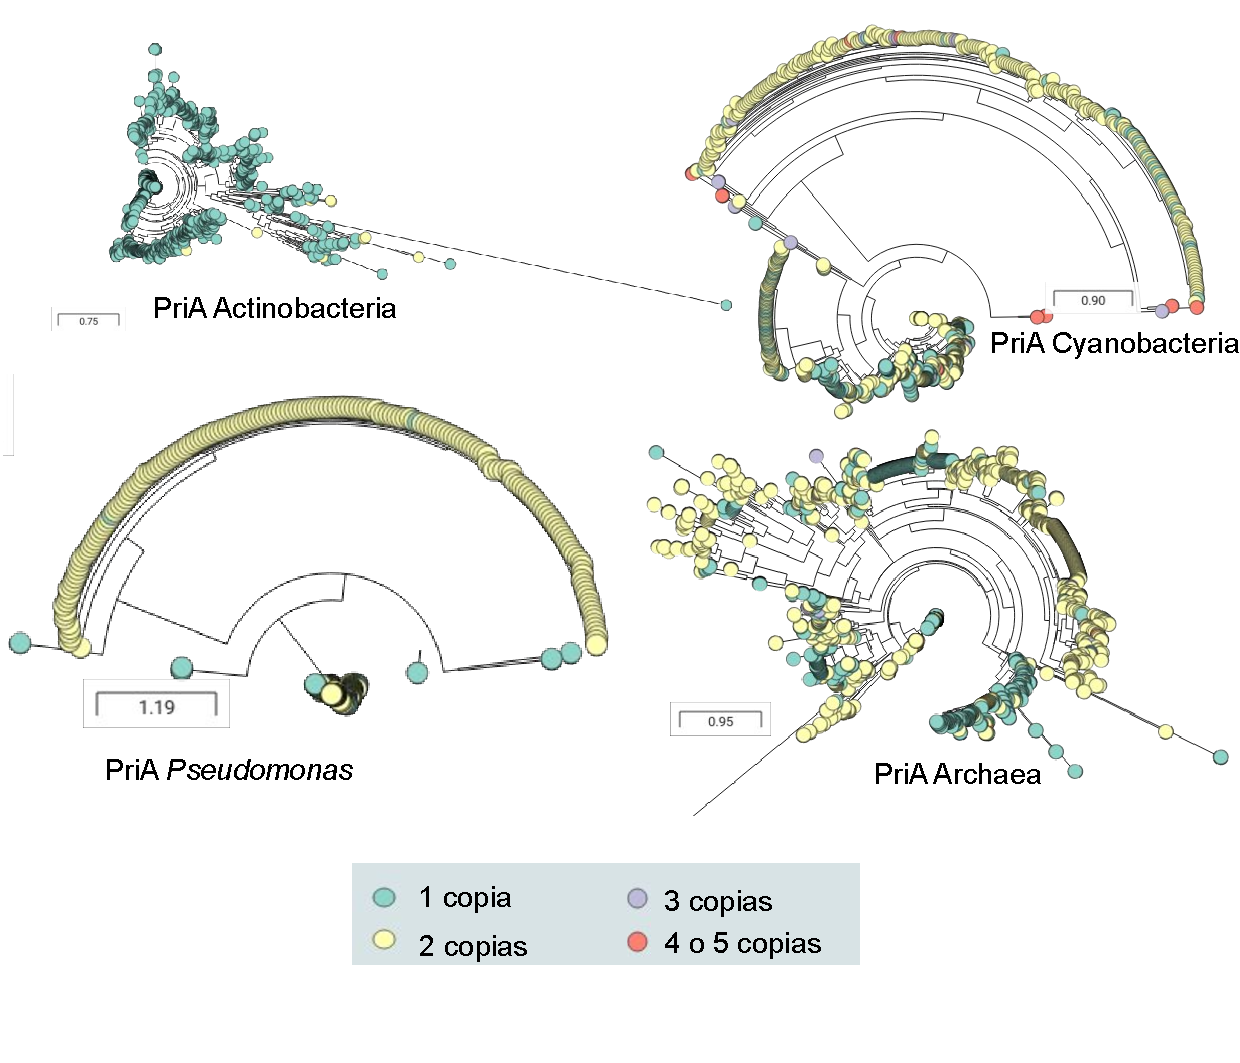
\includegraphics[angle = 0,scale = 0.8]{chapter4/PriAEvoMiningCopies.pdf}
\caption[Copias extras de PriA en Actinobacteria, Cyanobacteria, Pseudomonas y Archaea]{\footnotesize{}}
\label{fig:PriAEvoMiningCopies}
\end{figure}

Después de explorar cuáles organismos tienen expansiones de PriA, a
continuación se muestra en la \autoref{fig:PriATrees} el posible destino
metabólico de las copias extra de la familia. El árbl de Actinobacteria
está poblado de hojas rojas, es decir de PriA dedicadas al metabolismo
conservado, en este caso a las rutas de Histidina y Triptofano. Sin
embargo hay algunas hojas grises, como es el caso de los dos
\emph{Serenicoccus} mencionados previamente. Es posible que estas PriA
puedan tener funciones alternativas. Además, en Actinobacteria la PriA
de \emph{Janibacter Hoilley}, la rama más larga del árbol, es muy
divergente. Esto se debe a que existe una fusión de PriA con HisH, que
no parece ser un artefacto de anotación ya que hay otros
\emph{Janibacter} con PriA ligeramente más grandes que el promedio.

En Cyanobacteria hay pocas hojas verdes (EvoMining predictions) y no
están localizadas cerca de la HisA de saxitoxin, el BGC proveniente de
Cyanobacteria. En \emph{Pseudomonas} hay una gran población de
predicciones de EvoMining, pero son falsos positivos, ya que estas no
corresponden a una rama dedicada al metabolismo secundario, sino a la
rama de la ciclasa. En Archaea algunas de los hojas grises, es decir sin
destino metabólico conocido serán exploradas en la siguiente sección.

\begin{figure}[h!tbp]
\centering
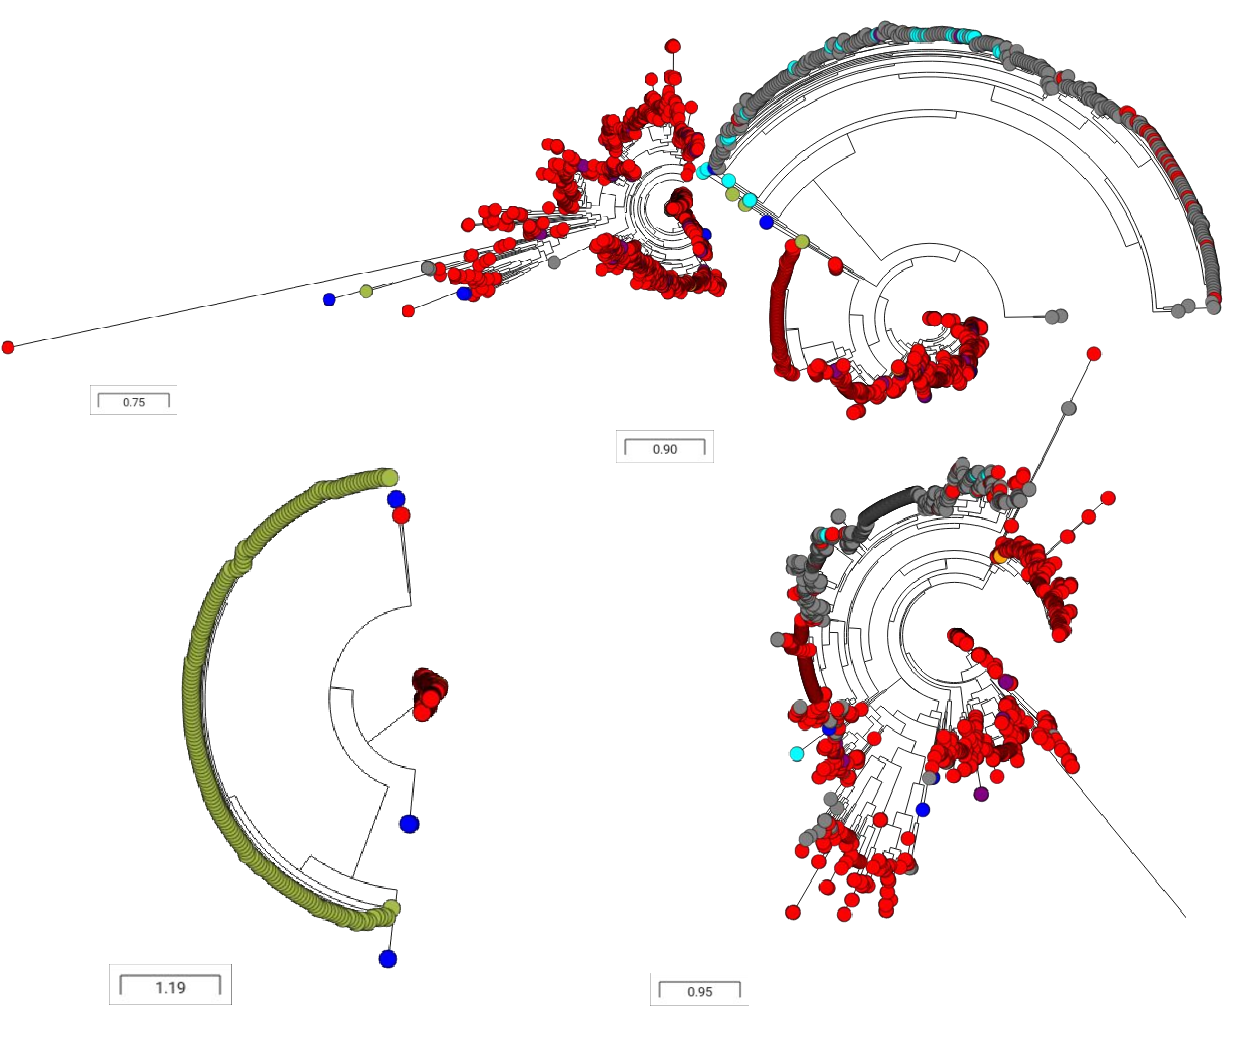
\includegraphics[angle = 0,scale = 0.8]{chapter4/PriAEvoMining.pdf}
\caption[Árboles de destino metabólico de PriA en Actinobacteria, Cyanobacteria, {Pseudomonas} y Archaea según EvoMining]{\footnotesize{Árboles de destino metabólico de PriA en Actinobacteria, Cyanobacteria, {Pseudomonas} y Archaea según EvoMining}}
\label{fig:PriATrees}
\end{figure}

Todos los reclutamientos (marcados en azul en el árbol) que tuvieron
estas expansiones en estos linajes genómicos están listados en la tabla
\autoref{tab:reclutamientos}. Entre ellos se encuentran dos toxinas de
Cyanobacteria{[}@moustafa\_origin\_2009{]}, un lipopolisacárido
producido por una Proteobacteria y un BGC productor de cloro
pentostatina producido en Actinobacteria {[}@gao\_biosynthesis\_2017{]}.

Table: Reclutamientos de expansiones de PriA en MIBiG
\label{tab:reclutamientos}\\
\($ \resizebox{\columnwidth}{!}{% \begin{tabular}{ l c r c c c c} \hline \\ [-1.5ex] &Compuesto&Actinobacteria&Cyanobacteria&Proteobacteria&Archaea&BGC origen&Clase \\ [1ex] & [saxitoxin](http://mibig.secondarymetabolites.org/repository/BGC0000188/index.html#cluster-1)&&\)Cylindrospermopsis\textasciitilde{}
raciborskii\$ T3\&\&\& Alcaloide \textbackslash{} {[}1ex{]} \&
\href{http://mibig.secondarymetabolites.org/repository/BGC0000928/index.html\#cluster-1}{toxin}\&\&\(Dolichospermum~circinale\)
AWQC131C\&\&\& Otros \textbackslash{} {[}1ex{]} \&
\href{http://mibig.secondarymetabolites.org/repository/BGC0000775/index.html\#cluster-1}{lipopolisacárido}
\& \& \& \& \(Legionella~pneumophila\) \& Sacarido \textbackslash{}
{[}1ex{]} \&
\href{http://mibig.secondarymetabolites.org/repository/BGC0001484/index.html\#cluster-1}{ada}\&\(Actinomadura\)
sp. ATCC 39365\&\&\&\& Otros \textbackslash{} {[}1ex{]}

\hline \textbackslash{} {[}-1.5ex{]} \hline
\textbackslash{}end\{tabular\}\} \%\} \$\$

La pentostatina es un atibiótico nucleosídico derivado de adenosina,
cuyo cluster es llamado \emph{ada} . La PriA del cluster \emph{ada} es
llamada \emph{adaK} y sí parece participar del cluster, ya que muestra
una isomerización sobre un sustrato similar a los nativos de PriA,
\autoref{fig:ada}, con un anillo de 5 carbonos, dos OH, un oxígeno y un
grupo fosfato . Esta isomerización es muy parecida a la que realiza PriA
sobre ProFAR y PRA. Esta PriA no es una copia extra, sino la copia única
de este organismo. Este contexto genómico no se encuentra conservado en
las copias vecinas en el árbol. Es relevante mencionar que la mutante de
PriA no suprime la producción de este antibiótico en \emph{Actinomadura}
sp. ATCC 39365, por lo que los autores especulan que otra enzima podría
estar realizando la isomerización redundantemente. \emph{Actinomadura}
no posee una copia de TrpF que sería el candidato inmediato.

\begin{figure}[h!tbp]
\centering
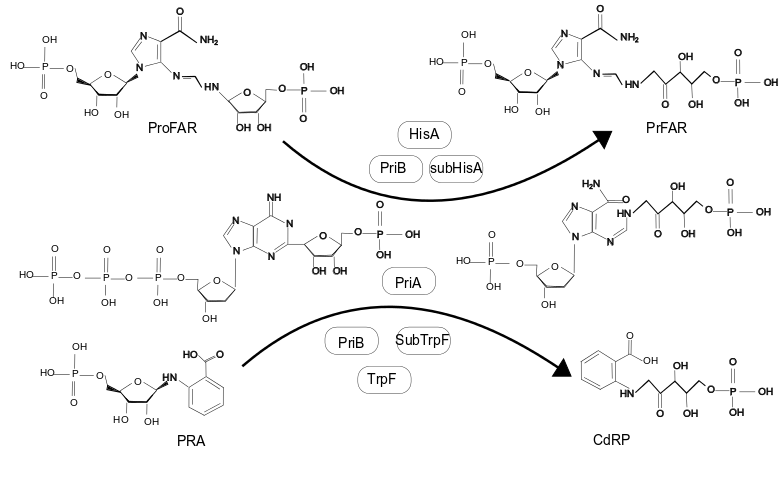
\includegraphics[angle = 0,scale = 0.6]{chapter4/ada.png}
\caption[PriA participa en la síntesis del antibiótico {ada} en {Actinomadura} ]{\footnotesize{PriA participa en la síntesis del antibiótico {ada} en {Actinomadura}. Los sustratos nativos de Pria, ProFAR y PRA son isomerizados de manera muy similar a un paso en la ruta de síntesis de {ada} }}
\label{fig:ada}
\end{figure}

Finalmente, los árboles que se produjeron por EvoMining están
disponibles para exploración interactiva en Microreact en los links de
la \autoref{tab:arboles}:

\begin{longtable}[]{@{}lc@{}}
\caption{Árboles EvoMining de PriA en MicroReact
\label{tab:arboles}}\tabularnewline
\toprule
Linaje & Link al árbol de EvoMining en Microreact\tabularnewline
\midrule
\endfirsthead
\toprule
Linaje & Link al árbol de EvoMining en Microreact\tabularnewline
\midrule
\endhead
Actinobacteria &
\href{https://microreact.org/project/7g2IGfkv9}{7g2IGfkv9}\tabularnewline
Cyanobacteria &
\href{https://microreact.org/project/qF6jWRMox}{qF6jWRMox}\tabularnewline
\emph{Pseudomonas} &
\href{https://microreact.org/project/ydff6DWqs}{ydff6DWqs}\tabularnewline
Archaea &
\href{https://microreact.org/project/Ig-m9Cm6f}{Ig-m9Cm6f}\tabularnewline
\bottomrule
\end{longtable}

\subsubsection{Análisis de contextos genómicos de PriA en distintos
linajes utilizando
CORASON}\label{analisis-de-contextos-genomicos-de-pria-en-distintos-linajes-utilizando-corason}

En Actinobacteria, se observó que todos los \emph{Streptomyces} tienen
el cluster de PriA parcialmente conservado con respecto al BGC de
\emph{Streptomyces coelicolor}. Ejemplos de ello son \emph{S. roseous},
\emph{S. sviceus}, \emph{S. sp C} y \emph{S. Mg1} donde genes tanto de
la ruta de histidina como de triptofano rodean a PriA. Otros como
\emph{S rimosus} , \emph{S HmicA12} y \emph{S. sp CT34} tienen los genes
de triptofano más alejados \autoref{fig:PriACORASON} . Como ya se
describió en la sección de EvoMining, el único organismo de este género
con una copia extra de PriA es \emph{Streptomyces} CT34. Esta copia
parece deberse a transferencia horizontal dado que su mejor hit en NCBI
proviene de una \emph{Lentzea}. Aún así parece ser un homólogo lejano ya
que tuvo 50\% de identidad en 98\% de cobertura con respecto a la copia
de \emph{Lentzea}. Otro caso interesante en Actinobacteria son las
Actinomaduras, ya que CORASON muestra que el cluster \emph{ada} no está
conservado en ellas (datos no mostrados). Además, también en
Actinobacteria CORASON muestra en \emph{Sporichthya polymorpha} DSM
43042 una PriA precedida por una NRPS, una enzima por excelencia de
productos naturales. En otros organismos antiSMASH predice que PriA
forma parte de clusters putativos, por ejemplo en \emph{Modestobacter
marinus} NC\_0179551, \emph{Geodermatophilus obscurus}, y en
\emph{Streptacidiphilus jeojiense}. Los contornos de los genes
reconocidos por antiSMASH como parte de un BGC son marcados en azul en
las figuras de CORASON.

En cuanto a Archaea, los contextos mostrados en los páneles b y c de la
\autoref{fig:PriACORASON} muestran que si bien existen algunos contextos
como el de ciertos \emph{Thermococcus} donde PriA está rodeada de genes
de histidina y triptofano, esta configuración no es la generalidad. Al
contrario, parece que no hay una configuración conservada que prevalezca
en todo Archaea. Esto puede deberse a que Archaea es un dominio, no un
phylum como Actinobacteria, y por tanto hay una mayor distancia entre
los organismos que la conforman.

\begin{figure}[h!tbp]
\centering
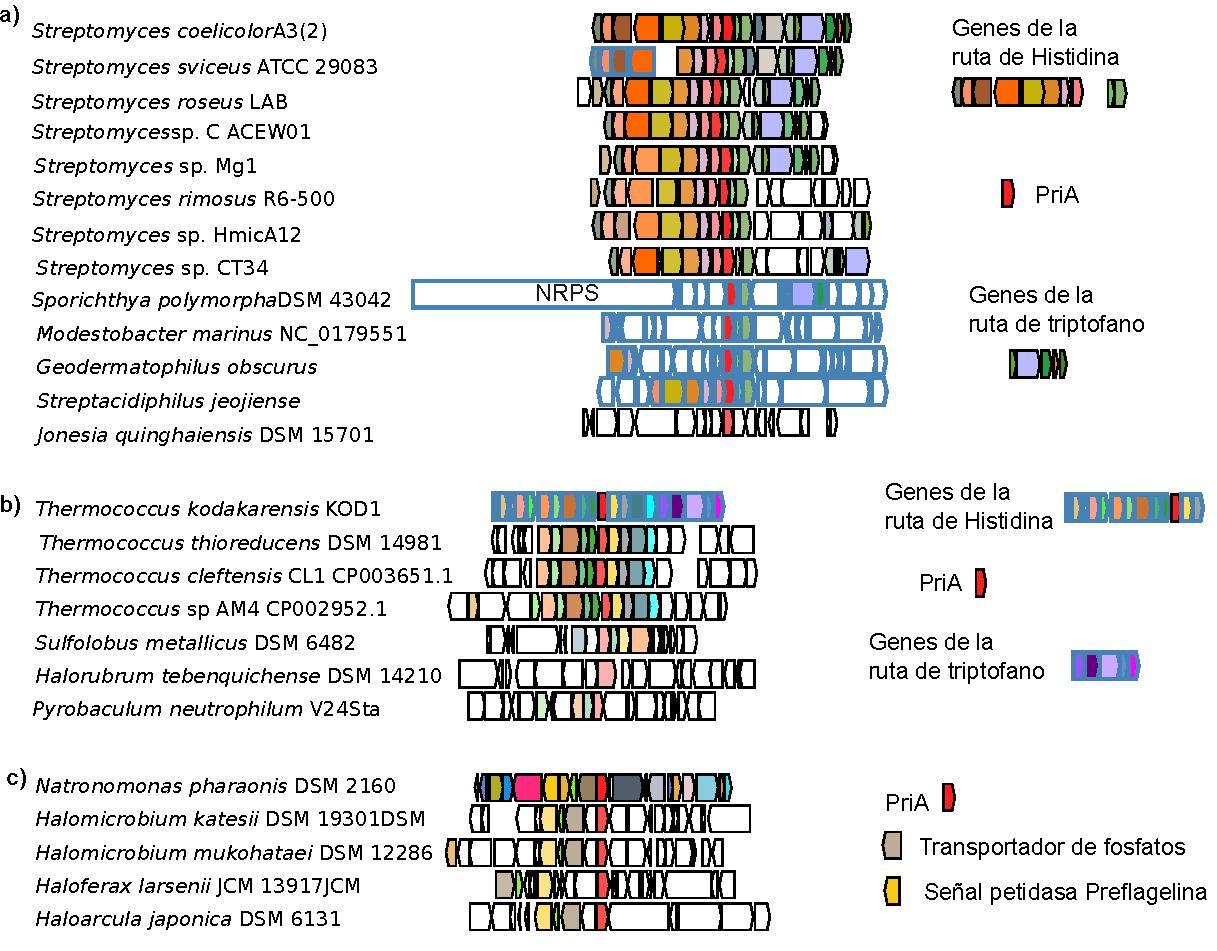
\includegraphics[angle = 0,scale = 0.7]{chapter4/CORASON/CORASON.pdf}
\caption[Contextos de PriA en Actinobacteria y Archaea]{\footnotesize{Contextos de PriA en Actinobacteria y Archaea}}
\label{fig:PriACORASON}
\end{figure}

En cuanto a PriA en Cyanobacteria la visualización de contextos
producida por CORASON tomando como referencia el cluster de saxitoxin,
muestra que las enzimas biosintéticas de ese no están conservadas en
otros organismos. Además en el lado izquierdo de la
\autoref{fig:saxitoxin} se muestra que la PriA del BGC saxitoxin no está
ubicada en una rama de PriA divergente, al contrario está en la parte
más conservada. Por estas razones es posible que PriA esté en la orilla
del BGC de saxitosin y más bien no participe en la síntesis de este
compuesto.

\begin{figure}[h!tbp]
\centering
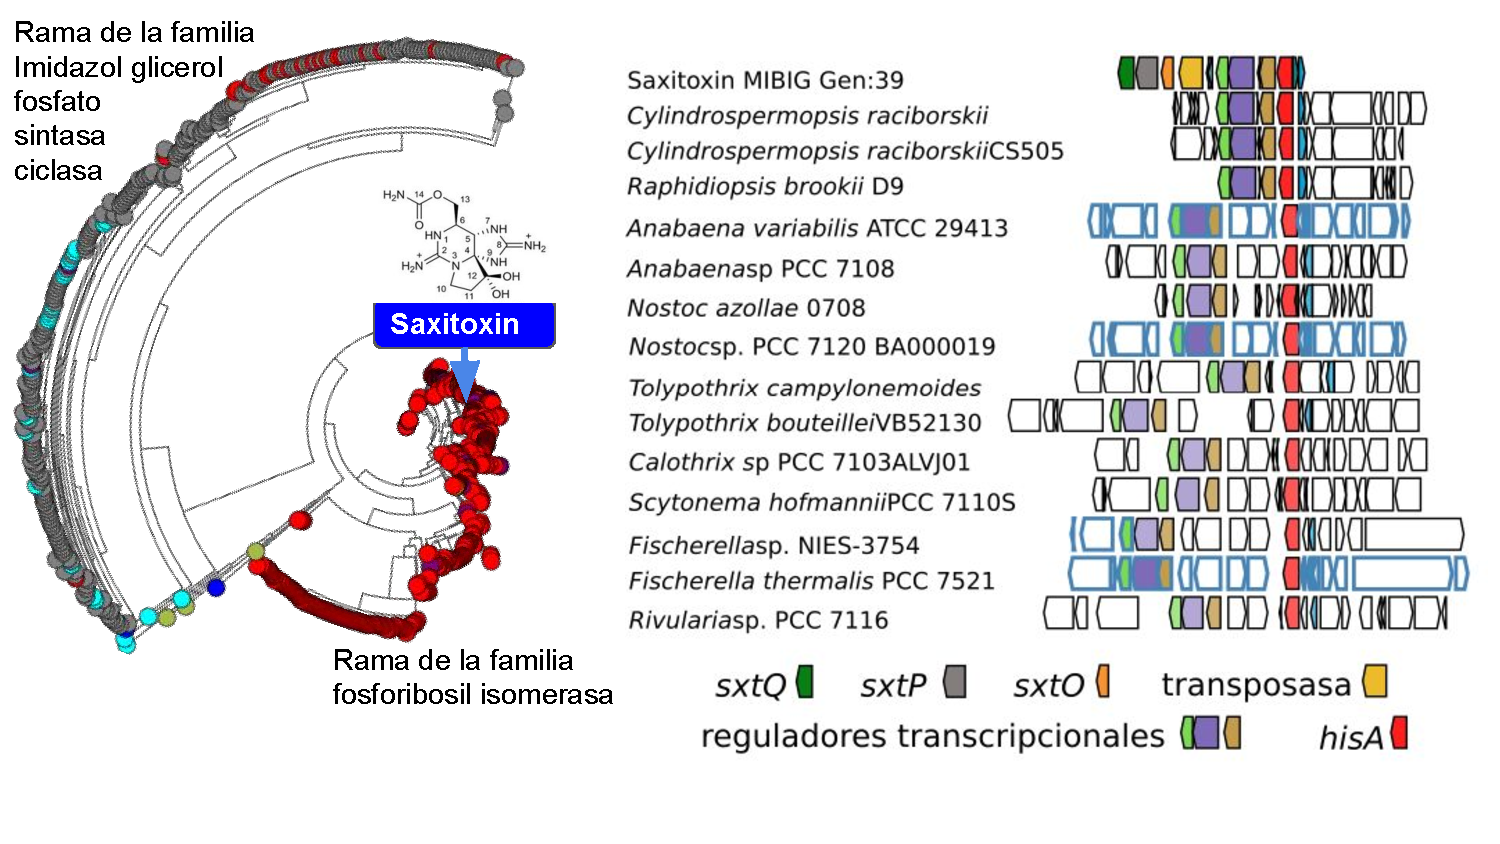
\includegraphics[angle = 0,scale = 0.7]{chapter4/CORASON/saxitoxin.pdf}
\caption[HisA en saxitoxin, un cluster de Cyanobacteria ]{\footnotesize{HisA en saxitoxin, un cluster de Cyanobacteria }}
\label{fig:saxitoxin}
\end{figure}

\subsection{El monitoreo en cambios de aminoácidos en PriA para estudiar
rutas evolutivas y reconstrucciones de la estructura
tridimensional.}\label{el-monitoreo-en-cambios-de-aminoacidos-en-pria-para-estudiar-rutas-evolutivas-y-reconstrucciones-de-la-estructura-tridimensional.}

En esta segunda sección concerniente a la familia PriA se busca
información contenida en la secuencia de aminoácidos. En la primera
parte se discute cómo en datos de evolución dirigida en el laboatorio no
se encontró ninguna trayectoria en donde algún paso incrementara la
actividad de PriA en sus dos sustratos nativos. En la segunda parte se
muestra una reconstrucción de la estructura tridimensional de PriA
basada en la covarianza de sus aminoácidos en secuencias del registro
evolutivo.

\subsubsection{Al transformar una subHisA en una PriA mediante
mutaciones no se observó ninguna trayectoria creciente para ambos
sustratos
(darwiniana)}\label{al-transformar-una-subhisa-en-una-pria-mediante-mutaciones-no-se-observo-ninguna-trayectoria-creciente-para-ambos-sustratos-darwiniana}

En esta sección analizamos cómo cambia la capacidad catalítica de PriA
sobre un sustrato mientras se varía la del otro. Para ello se utilizaron
datos de mutantes de subHisA de \emph{Corynebacterium diphteriae}. Estas
mediciones de cinéticas enzimáticas fueron obtenidos del trabajo de
tesis de Lianet Noda {[}@noda\_tesis\_2012{]}. A partir de la secuencia
original que se mostró es una subHisA, se realizaron mutantes con el
objetivo de alcanzar la promiscuidad, es decir de convertir la enzima
subHisA en una PriA. Se comenzó con diferentes mutantes puntuales
adicionando una mutación cada vez, hasta llegar a una con 11 mutaciones.
En esta colección de mutantes varias ganaron la función de PRA
isomerasa, a distintos niveles. La que alcanzó mayor actividad PRA
isomerasa fue la \(9.3\), una variante con nueve mutaciones. En estos
datos quedaba pendiente la exploración de las rutas, es decir cómo es el
camino desde una mutante sencilla hasta una múltiple ¿cuántas rutas son
posibles? ¿Existe alguna tendencia en ciertos momentos de la ruta sobre
el incremento/decremento de alguna de las dos funciones?

Asi pues se desarrolló un
\href{https://github.com/nselem/perlas/tree/master/LiaTrayectory}{script}
utilizando recursividad para reconstruir todas las rutas posibles. El
total de rutas calculadas hasta la mutación 11 fue de 2928 caminos, las
rutas posibles hasta la mutante 9.3 son 790. Estas rutas son mostradas
en la \autoref{fig:PriARutas}.

\begin{figure}[h!tbp]
\centering
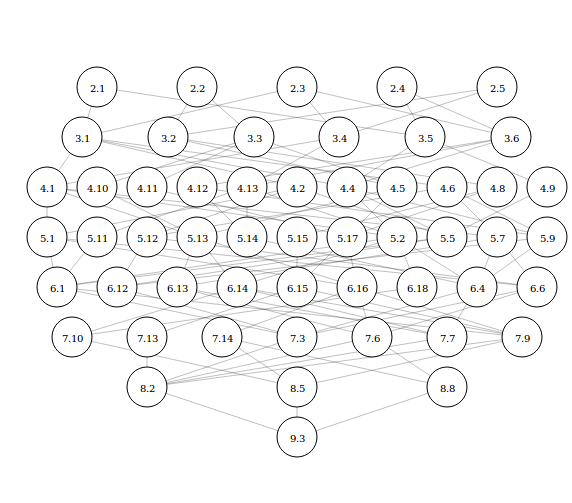
\includegraphics[angle = 0,scale = 0.6]{conclusion/Solocirculos.png}
\caption[Rutas desde una subHisA hasta una variante con 9 mutaciones]{\footnotesize{Rutas desde una subHisA hasta una variante con 9 mutaciones. En cada círculo el primer dígito indica el número de mutaciones}}
\label{fig:PriARutas}
\end{figure}

Al analizar los cambios sufridos en cada actividad en cada paso de cada
ruta se descubrió que no existe en ellas una trayectoria no decreciente
para ningún sustratos. Como ejemplo, en la \autoref{fig:PriARutas} se
muestran las rutas donde cada mutante mantiene un nível mínimo de
actividad de ProFAR isomerasa
(\(\frac{K_{cat}}{K_m} PriA_{ProFAR} \ge .004\)). En azul sólido se ven
los incrementos en PRA y en rojo sólido los incrementos en ProFAR. Las
líneas punteadas indican que la actividad decreció en ese paso de la
ruta. Entre una y cuatro mutaciones el azul sólido es predominante, es
decir se incrementa la actividad para PRA, pero entre 4 y 5 mutaciones
ningún paso incrementa la actividad de PRA y en cambio sí se incrementa
la actividad para ProFAR, esta figura sugiere que al mejorar una
actividad se compromete el mejoramiento de la otra. En este ejemplo, las
mutaciones puntuales que llevan a una enzima monofuncional a adquirir
promiscuidad no mantienen una tendencia no decreciente de principio a
fin sobre ninguna ruta en ninguna de las dos reacciones isomerización de
PRA e isomerización de ProFAR. Este tipo de trayectorias se conoce como
no darwininana ya que siempre existe algún paso donde decrece alguna de
las actividades.

\begin{figure}[h!tbp]
\centering
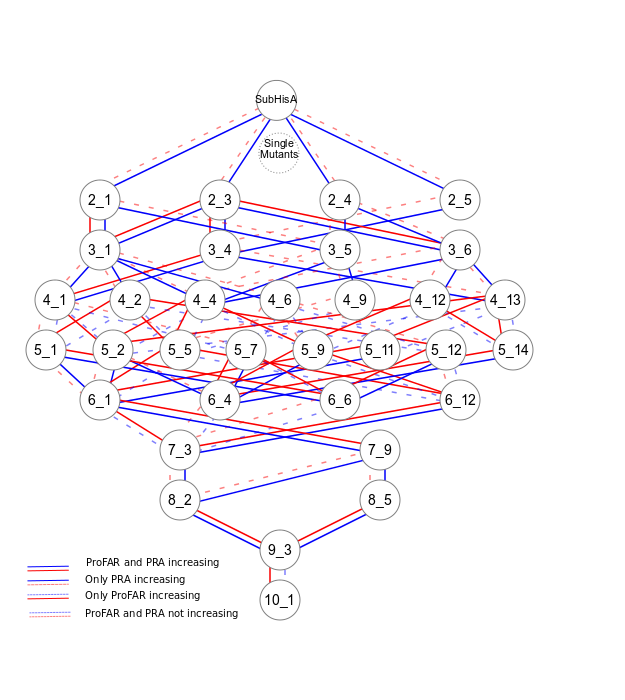
\includegraphics[angle = 0,scale = 0.8]{chapter4/LianetFiguras/SolocirculosPRA_PRO_RUTAS_10_1_r002.png}
\caption[Positive increments on PRA]{\footnotesize{Rutas de evolución dirigida para ganar la función PRA. En la figura se muestra como la mayoría de los pasos que incrementan una función hacer decrecer la capacidad catalítica de la otra. }}
\label{fig:PRARutas}
\end{figure}

\subsubsection{Los residuos que covarían en el registro evolutivo de
PriA permiten una reconstrucción aproximada de su estructura
tridimensional}\label{los-residuos-que-covarian-en-el-registro-evolutivo-de-pria-permiten-una-reconstruccion-aproximada-de-su-estructura-tridimensional}

El estudio de la evolución de PriA en la sección anterior nos
proporcionó el aprendizaje de que para adquirir una actividad el camino
no es estrictamente creciente. En cambio, suele haber pasos donde alguna
de las dos actividades baja. En esta sección utilizaremos el registro
evolutivo resultado de millones de años, tomaremos miles de homólogos de
PriA para inferir la estructura tridimensional de una secuencia.
Evcouplings es un método que considera las secuencias génicas existentes
como experimentos exitosos de la naturaleza. Con esta información
obtiene la covariación entre pares de aminoácidos de las secuencias
existentes en el registro evolutivo. Los pares fuertemente relacionados
se denominan acoplamientos, estos acoplamientos a menudo están cerca
físicamente en la estructura terciaria de la proteína. Se ha demostrado
que muchas proteínas contienen suficientes acoplamientos distribuidos
ampliamente en toda la secuencia, de forma que con ellos es posible la
reconstrucción de su estructura tridimensional
{[}@marks\_protein\_2011{]}. En esta sección se aplicará EVcouplings
para reconstruir la estructura tridimensional de PriA.

Las diferencias a nivel estructural pueden amplificar la información
proporcionada por variaciones a nivel de secuencia. Por este motivo se
decidió implementar Evcouplings {[}@marks\_protein\_2011{]}, para poder
aplicarlo a la familia PriA. Este método es de difícil instalación ya
que tiene muchas dependencias, por ello desarrollé un contenedor docker
donde las dependencias y el software quedan instalados. Este desarrollo
fue incluido por los desarrolladores originales como sugerencia de
instalación.\\
El contenedor docker implementa EVcouplings python framework
{[}@hopf\_evcouplings\_2019{]} que comprende cinco etapas para estudiar
el análisis de coevolución de residuos de una familia de proteínas.
Estas etapas son i) Alineado, ii) análisis de acoplamiento, iii)
plegamiento basado en acoplamientos iv) análisis de mutación y v)
comparación con estructuras conocidas.

EVcouplings fue aplicado a PriA de Streptomyces coelicolor con
identificador de Uniprot HIS4\_STRCO. Las secuencias para las
alineaciones se recuperaron automáticamente de Uniprot, otros parámetros
se dejaron con la configuración inicial del archivo de configuración.
Como resultado se modeló la estructura de PriA con los acoplamientos de
sus aminoácidos. Una comparación con una estructura cristalográfica es
mostrada en la \autoref{fig:CouplingsFoldingPriA}

La estructura reconstruida es parecida, pero para obtener mejor
definición es posible que se deba refinar la selección de las secuencias
del alineamiento, diferenciando entre secuencias conocidas de PriA,
subHisA, PriB y subTrpF.

\begin{figure}[h!tbp]
\centering
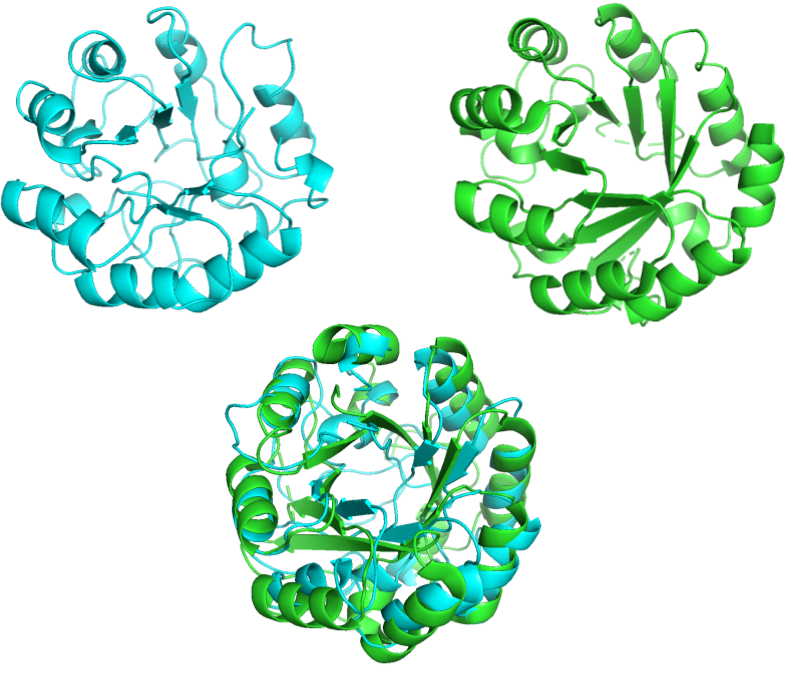
\includegraphics[angle = 0,scale = .5]{chapter4/Couplings/PriACouplingFoldings.png}
\caption[Superposición de estructura de PriA generado por Folding con la estructura cristalográfica]{\footnotesize{Comparación de estructura de PriA de {Streptomyces} {coelicolor} generada por EVcouplings con la estructura cristalográfica}}
\label{fig:CouplingsFoldingPriA}
\end{figure}

Finalmente los aminoácidos utilizados en la evolución dirigida de la
sección anterior fueron comparados con los provistos por EVCouplings
como altamente partícipes en la covariación. Los 10 con más
acoplamientos fueron 90L, 117V, 127V, 48W, 208I, 87D, 135T, 21V, 109E.
Sólo el 21V es parte los aminoácidos mutados en el estudio previament
descrito. En la \autoref{tab:aminoacidos} se muestra en la primera
columna los aminoácidos variados en el estudio de mutación dirigida en
\emph{Corynebacterium}, en la segunda columna el aminoácido
correspondiente en la secuencia de \emph{Streptomyces coelicolor} y
finalmente su correspondiente acoplamiento más significativo.\\

\begin{longtable}[]{@{}ccc@{}}
\caption{Árboles EvoMining de PriA en MicroReact
\label{tab:aminoacidos}}\tabularnewline
\toprule
\emph{Corynebacterium} & \emph{Streptomyces} & Acoplamiento más
relevante\tabularnewline
\midrule
\endfirsthead
\toprule
\emph{Corynebacterium} & \emph{Streptomyces} & Acoplamiento más
relevante\tabularnewline
\midrule
\endhead
D20V & 21V & 173T\tabularnewline
L48I & 49L & 76I\tabularnewline
F50L & 51L & 70V\tabularnewline
M66I & 67I & 80L\tabularnewline
T80S & 81S & 102N\tabularnewline
A97C & 98C & 107A\tabularnewline
D127A & 128G & 164V\tabularnewline
A129D & 130D & 168I\tabularnewline
T139L & 136L & 151T\tabularnewline
Y214L & 211Y & -\tabularnewline
E230A & 227A & 234E\tabularnewline
\bottomrule
\end{longtable}

Una forma gráfica de ver esta tabla es la \autoref{fig:couplings}. En
las líneas naranjas se muestra como el aminoácido 21D tiene un
acoplamiento con el 173T, que está muy cerca del 175D que ha sido
asociado con la actividad de isomerización de PRA, pero no de ProFAR.

\begin{figure}[h!tbp]
\centering
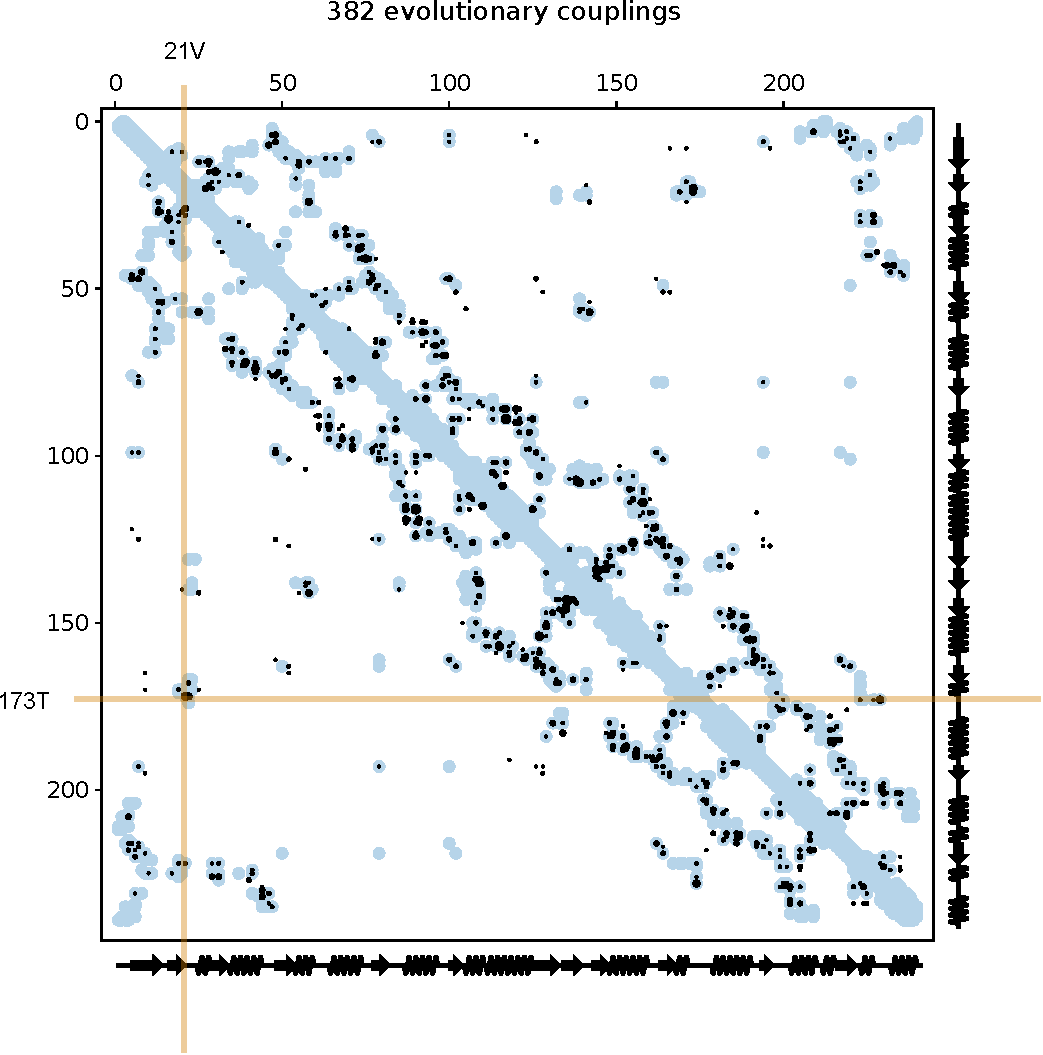
\includegraphics[angle = 0,scale = .5]{chapter4/Couplings/HIS4_STRCO_1-200/align/couplings.pdf}
\caption[Visualización de los acoplamientos en la familia PriA]{\footnotesize{Visualización de los acoplamientos en la familia PriA}}
\label{fig:couplings}
\end{figure}

Además se investigaron los aminoácidos catalíticos D130
{[}@due\_bisubstrate\_2011{]} y D175 reportados en \emph{Mycobacterium
tuberculosis}{[}@verduzco-castro\_co-occurrence\_2016{]} que
corresponden a en \emph{S coelicolor} D11, D131 y D171. Se econtró que
existe un conjunto de secuencias donde estos residuos no están presentes
\autoref{fig:Alineamiento}. La mayoría de estassecuencias es fuera del
phylum Actinobacteria, como PSeudomonas, Cyanobacteria, Enterobacteria,
Proteobacteria y Chloroflexi. Sin embargo, interesantemente se
encontraron 159 Corynebacterium, 49 Streptomyces y 2 Actinokineospora
sin 131D, entre ellos el ya mencionado \emph{Streptomyces CT 34} y
\emph{Streptomyces rimosus} . En Corynebacterium se encuentra localizada
la familia subHisA y en Streptomyces la familia PriB, la variabilidad
mostrada en estos géneros podría estar relacionada con la existencia de
estas familias. A futuro, para obtener resultados exclusivos sobre la
covariación de residuos en Actinobacteria, se debe proveer un
alineamiento exclusivo de Actinobacteria.

\begin{figure}[h!tbp]
\centering
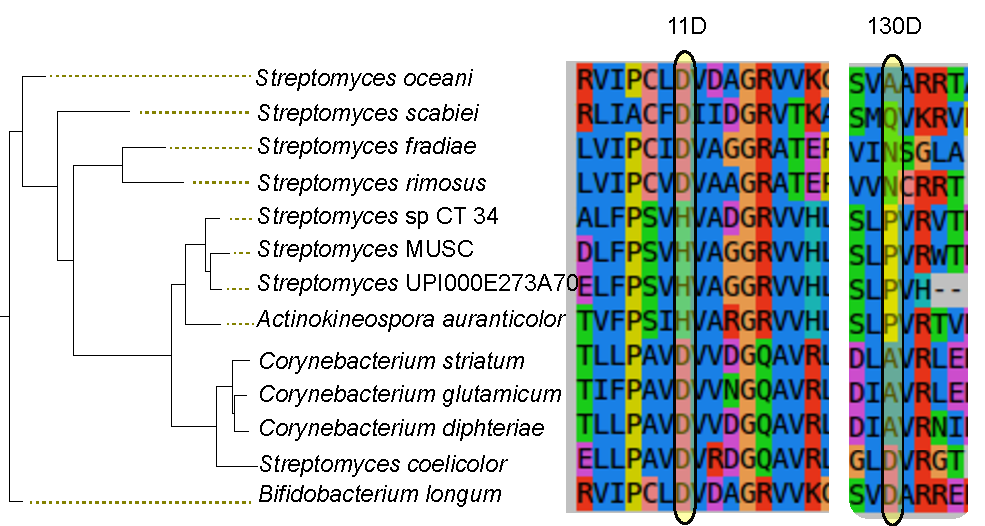
\includegraphics[angle = 0,scale = .5]{chapter4/Couplings/HIS4_STRCO_1-200/align/alineamiento.pdf}
\caption[Miembros de PriA que poseen variantes los residuos catalíticos D11, D130]{\footnotesize{Miembros de PriA que poseen variantes los residuos catalíticos D11, D130}}
\label{fig:Alineamiento}
\end{figure}

Finalmente la predicción del efecto de una mutacion para cada posición
de la secuencia para cada aminoacido podemos verlo en la siguiente
\autoref{fig:CouplingsMutationsPriA}

\begin{figure}[h!tbp]
\centering
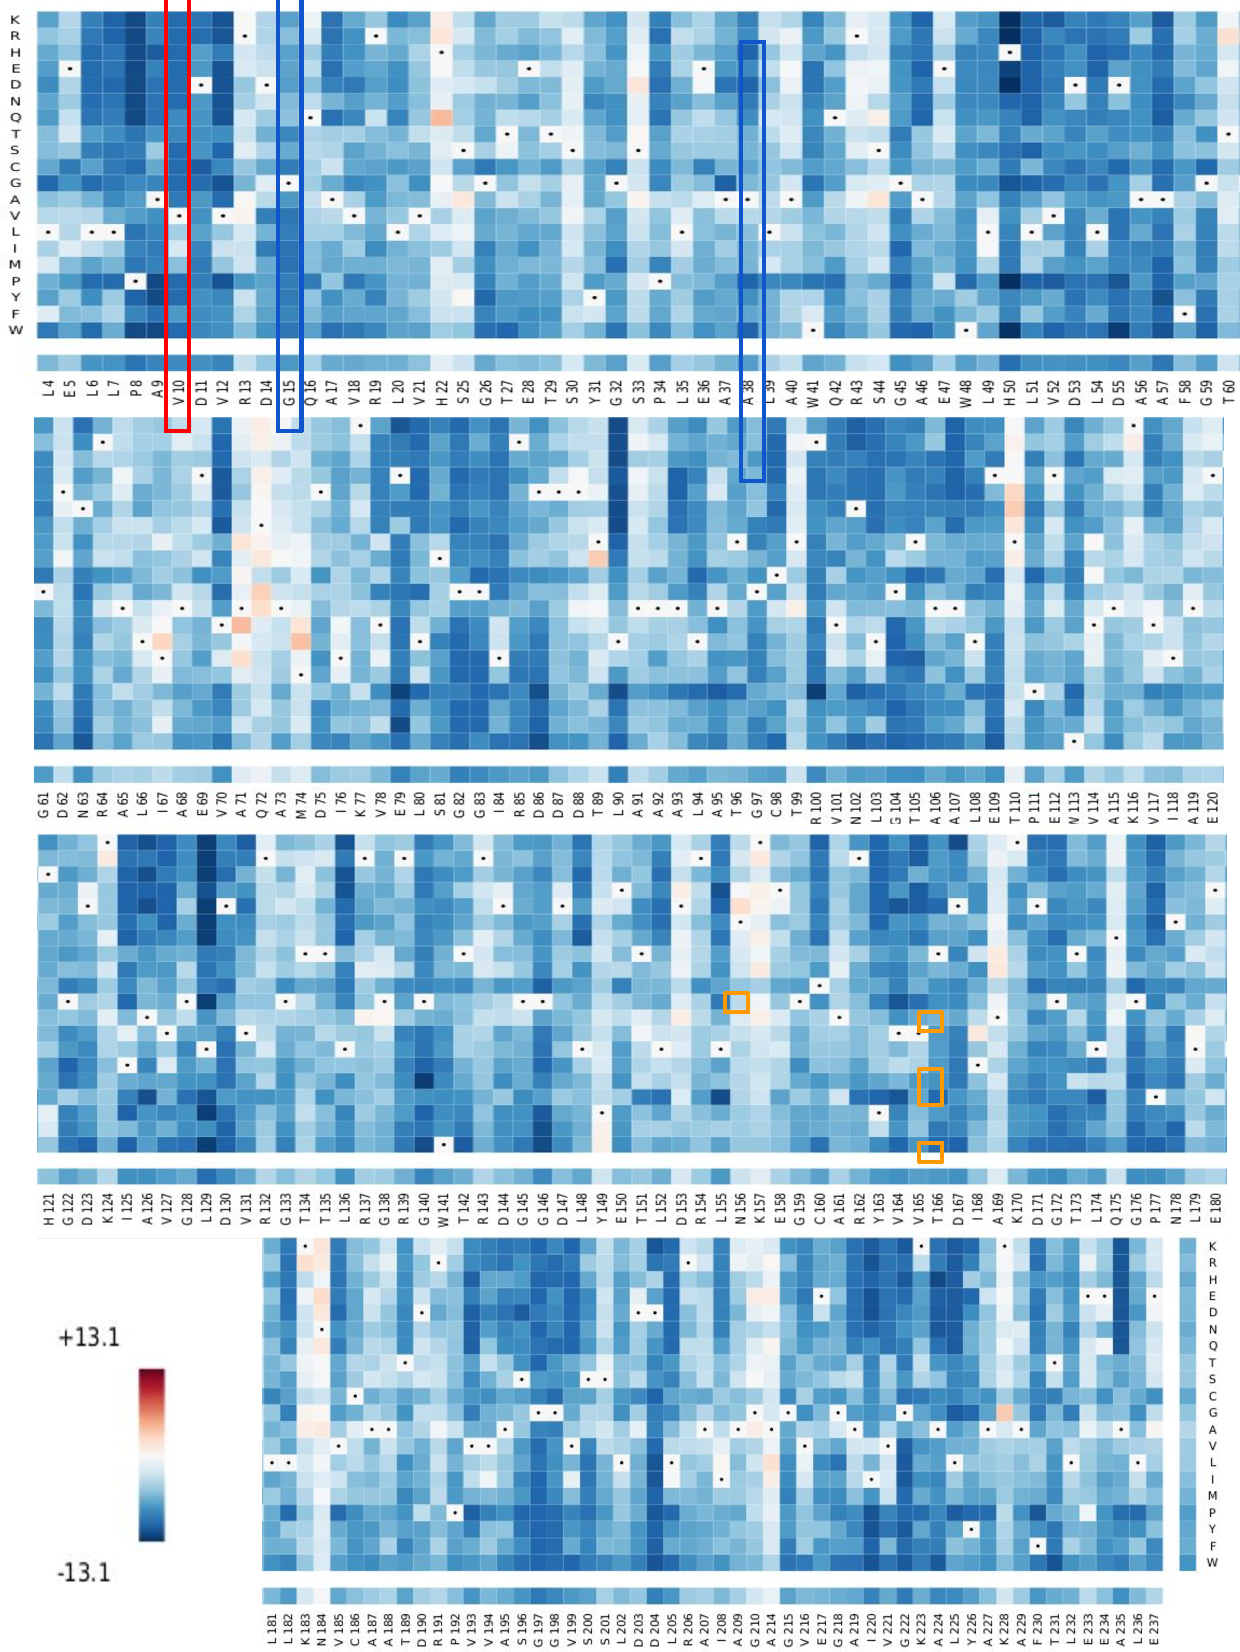
\includegraphics[angle = 0,scale = .8]{chapter4/Couplings/PriAMutations.pdf}
\caption[Tendencia de mutaciones observada en secuencias de PriA]{\footnotesize{}}
\label{fig:CouplingsMutationsPriA}
\end{figure}

\subsection{Afinidad de enzimas selectas por sustratos químicamente
parecidos a PRA y
PROFAR}\label{afinidad-de-enzimas-selectas-por-sustratos-quimicamente-parecidos-a-pra-y-profar}

Además de los sustratos conocidos ProFAR y PRA en los que PriA es capaz
de realizar una isomerización, es posible que PriA pueda ser promiscua
en otros sustratos. De hecho como se vio en la sección de EvoMining de
este capítulo, PriA parece participar en la síntesis del antibiótico
pentostaina \emph{ada}. Tomando este ejemplo como inspiración, se
colectaron en la literatura sustratos químicamente parecidos a ProFAR y
PRA \autoref{fig:Eschema1},
\autoref{fig:Eschema2},\autoref{fig:Eschema3},\autoref{fig:Eschema4}.
Así pues, esta sección buscará mostrar sustratos parecidos a los nativos
de PriA para posteriormente probar alguno en copias selectas de PriA
provenientes de diversos organismos.

Se seleccionaron veinte sustratos para realizar docking entre ellos y
las estructuras de las secuencias de PriA S1, S2, \ldots{} S20 sustratos
fueron recolectados de la literatura y las predicciones de la
quimioinformática. S3 PRA y S7 PROFAR son sustratos nativos, S13-S16 son
sustratos activados por la luz, S17 PRAP, S18 Compuesto V, se
encontraron en la literatura, S6 GMP, S11 GTP y otros fueron sugeridos
por chemioinformatics. Para tener una diea de la diversidad de estos
sustratos, se realizó entre ellos, un cálculo de distancias de Tanimoto.

\begin{figure}[h!tbp]
\centering
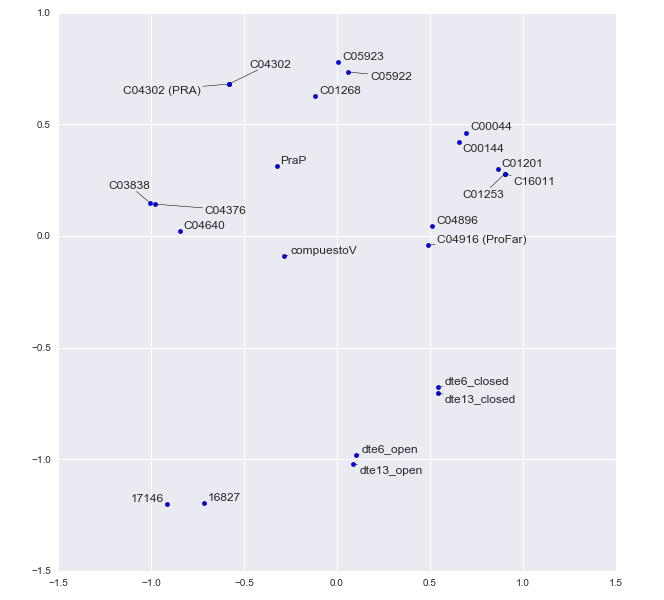
\includegraphics[angle = 0,scale = 0.4]{chapter4/SubstratesClustering.png}
\caption[Clustering de sustratos de acuerdo a sus distancias de Tanimoto]{\footnotesize{Clustering de sustratos de acuerdo a sus distancias de Tanimoto}}
\label{fig:tanimoto}
\end{figure}

\clearpage  

\begin{figure}[h!tbp]
\centering
\includegraphics[angle = 0,scale = .8]{chapter4/SustratosQuimicos.pdf}
\caption[Substatos químicamente similares a los sustratos de PriA (parte 1)]{\footnotesize{Substatos químicamente similares a los sustratos de PriA (parte 1)}}
\label{fig:Eschema1}
\end{figure}

\begin{figure}[h!tbp]
\centering
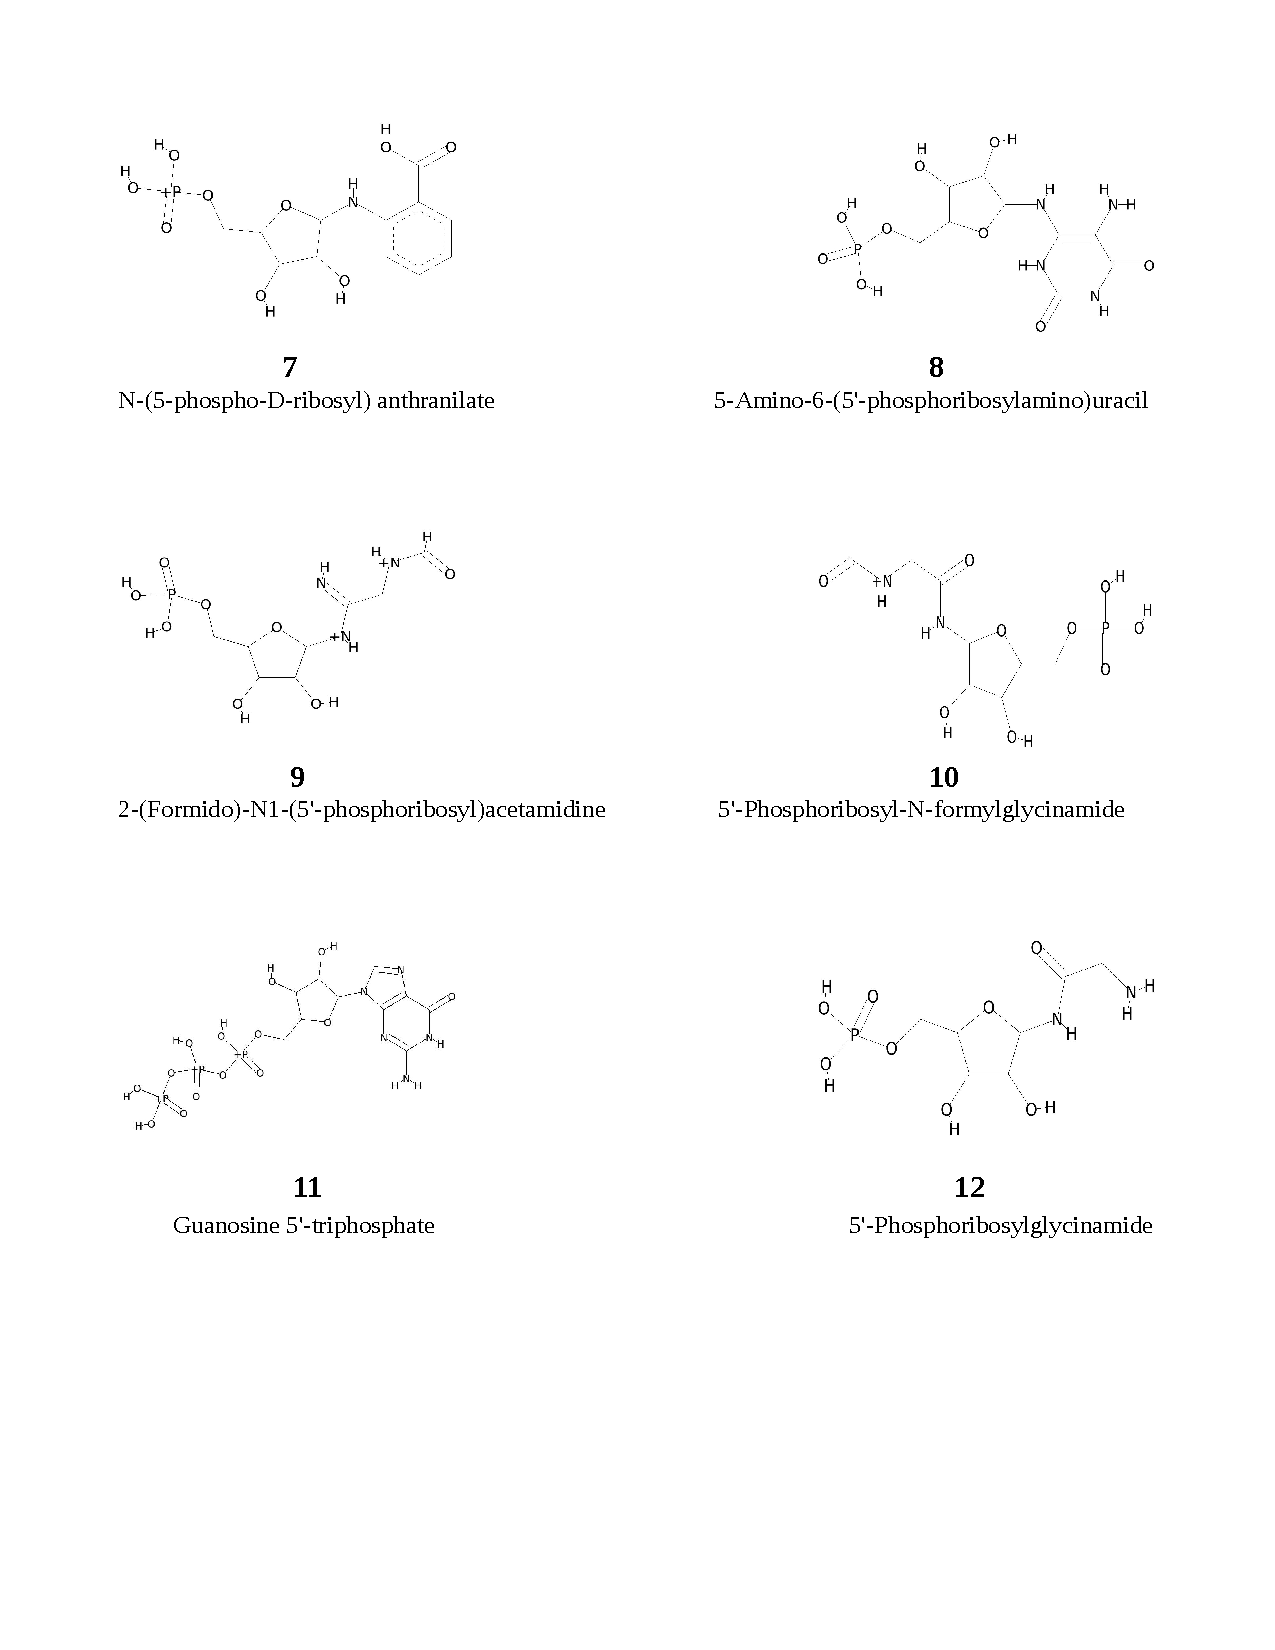
\includegraphics[angle = 0,scale = .8]{chapter4/esquema_quimico-2-2.pdf}
\caption[Substatos químicamente similares a los sustratos de PriA (parte 2)]{\footnotesize{Substatos químicamente similares a los sustratos de PriA (parte 2)}}
\label{fig:Eschema2}
\end{figure}

\begin{figure}[h!tbp]
\centering
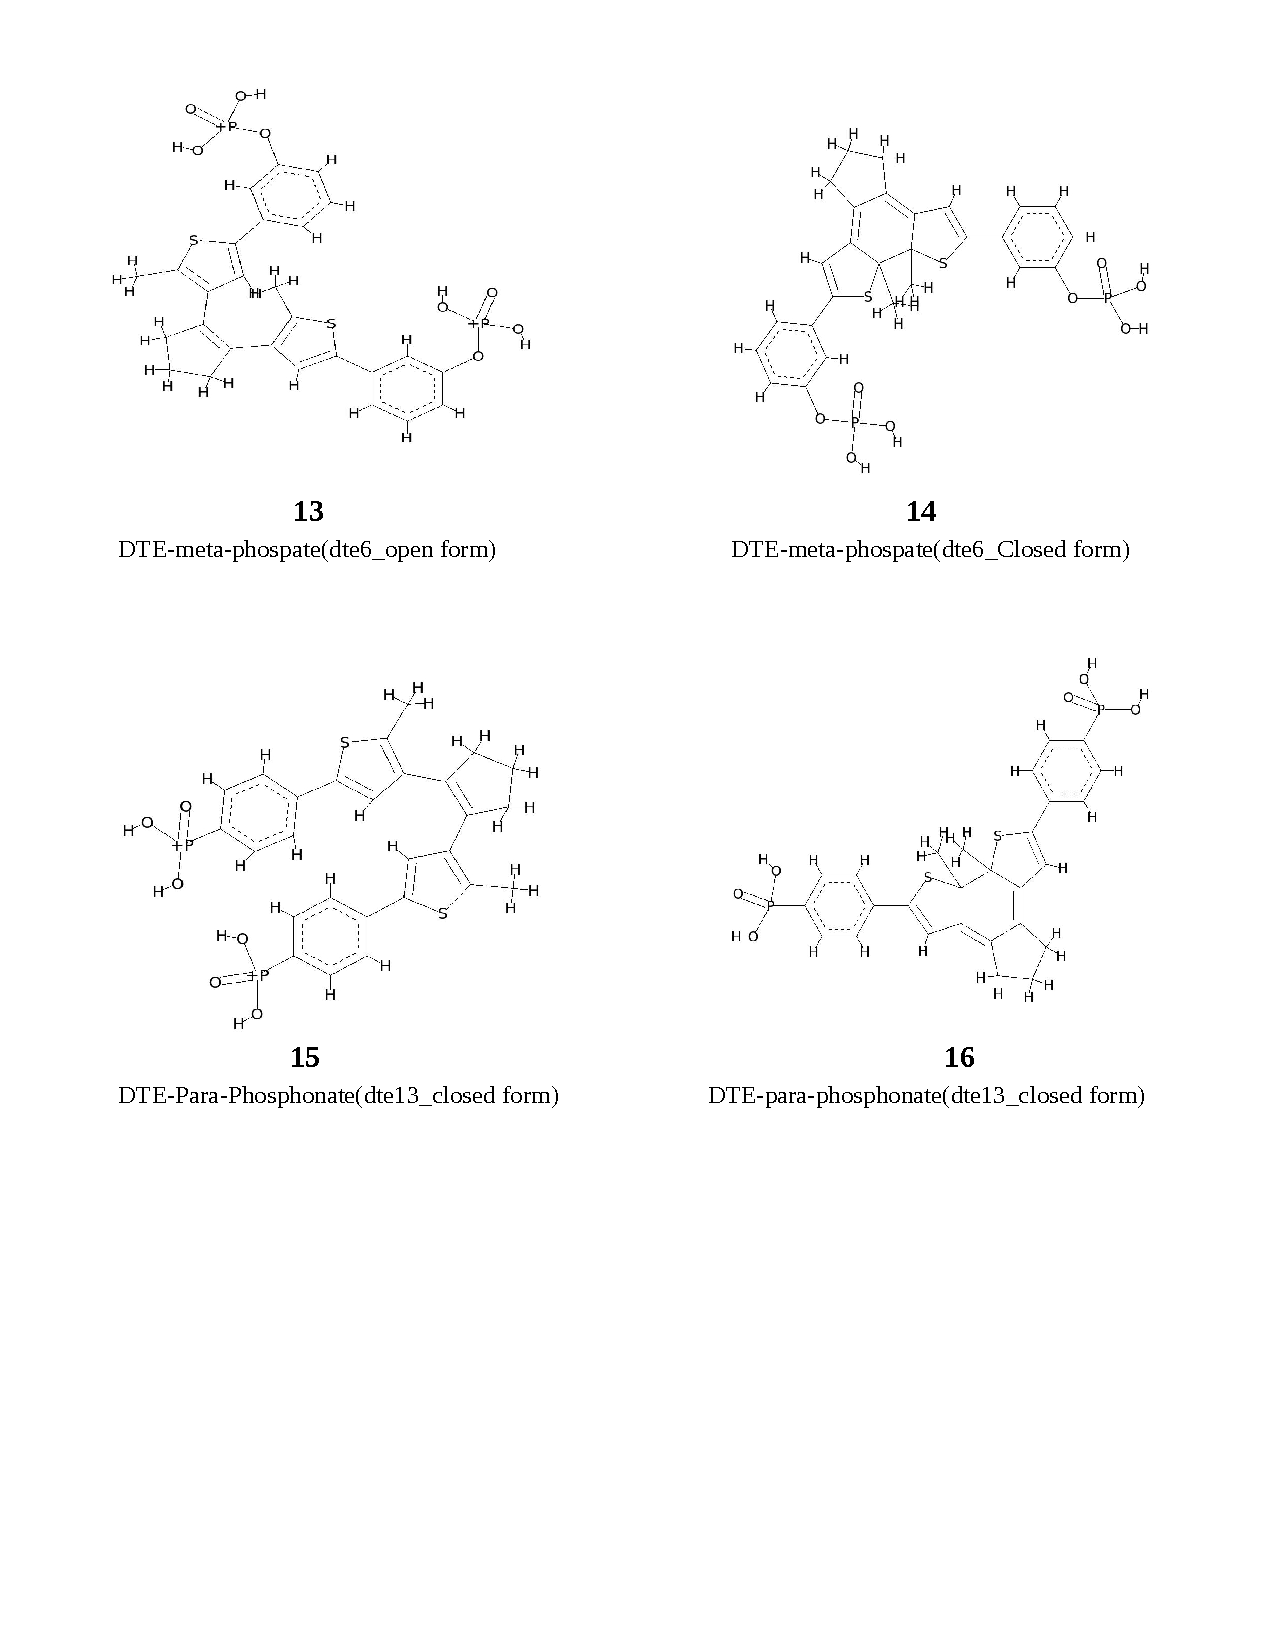
\includegraphics[angle = 0,scale = .8]{chapter4/esquema_quimico-3-3.pdf}
\caption[Substatos químicamente similares a los sustratos de PriA (parte 3)]{\footnotesize{Substatos químicamente similares a los sustratos de PriA (parte 3)}}
\label{fig:Eschema3}
\end{figure}

\begin{figure}[h!tbp]
\centering
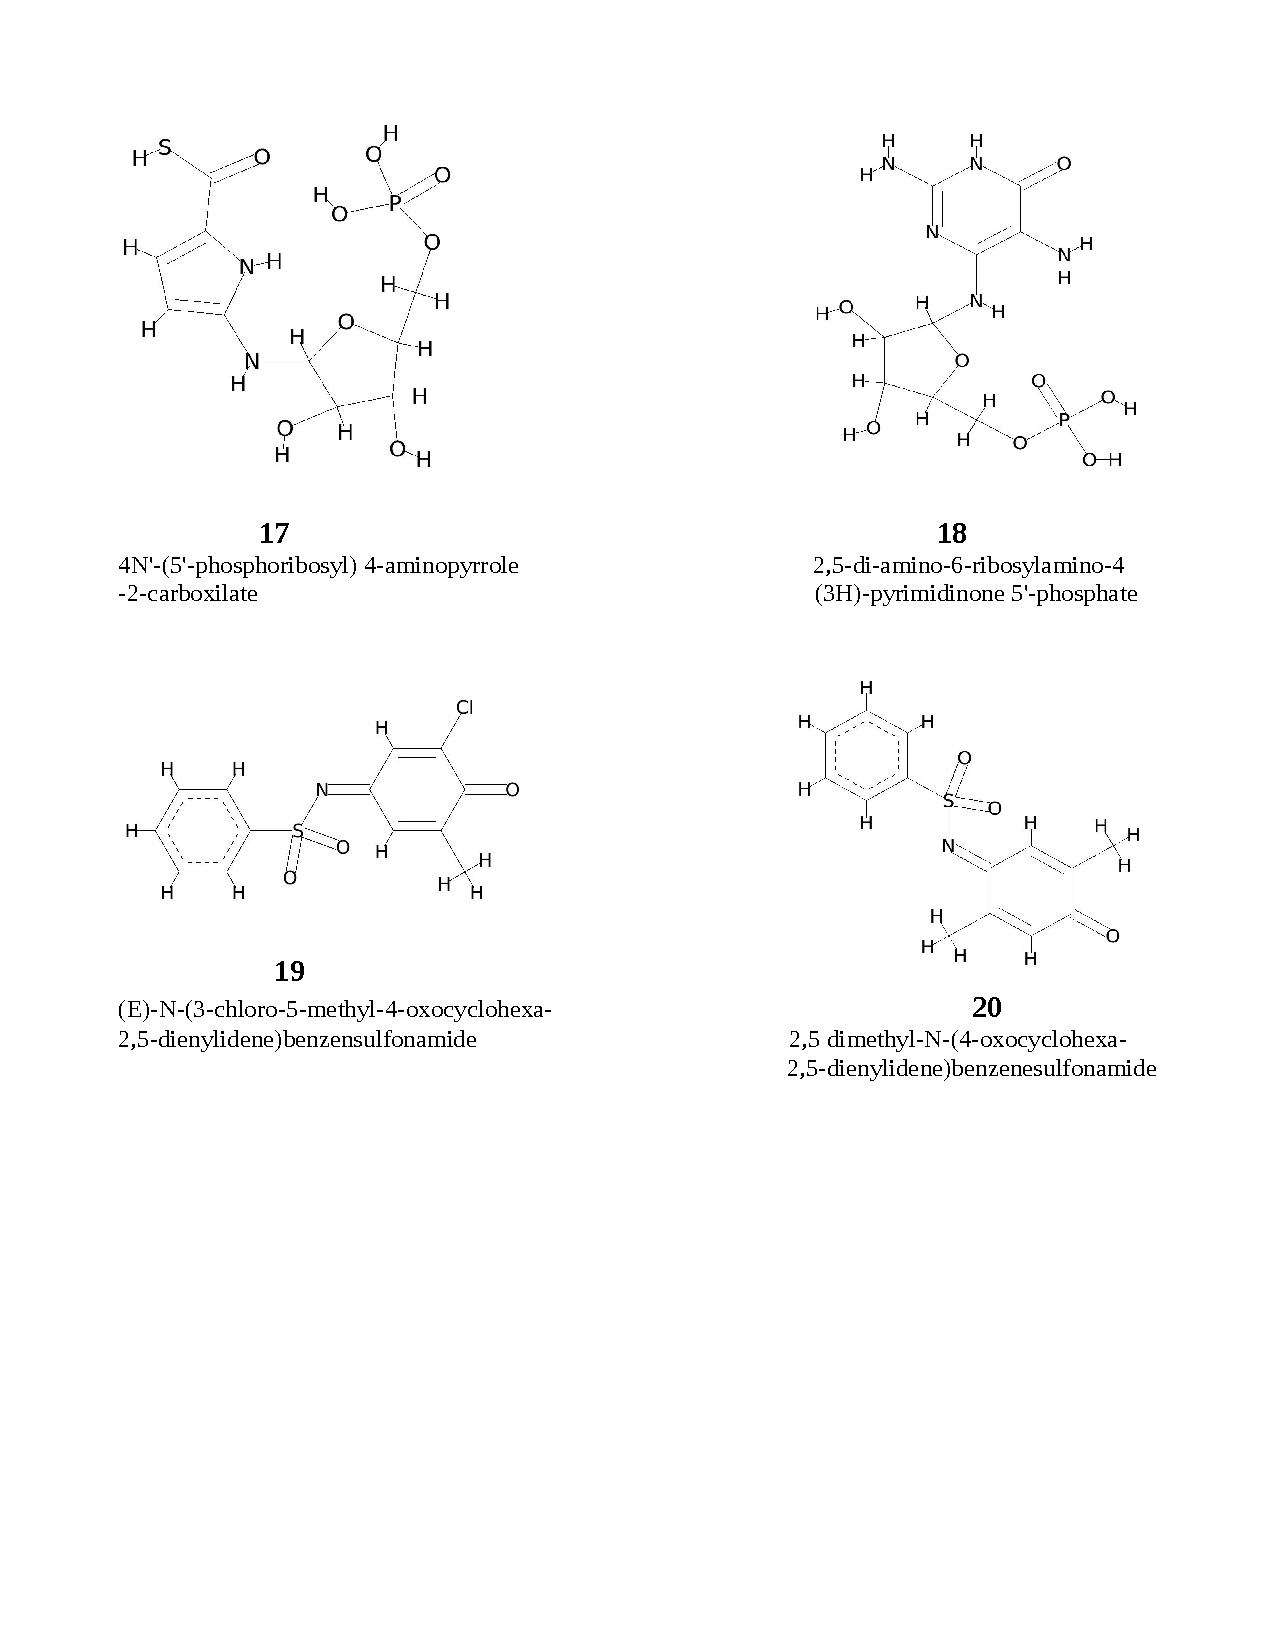
\includegraphics[angle = 0,scale = .8]{chapter4/esquema_quimico-4-4.pdf}
\caption[Substatos químicamente similares a los sustratos de PriA (parte 4)]{\footnotesize{Substatos químicamente similares a los sustratos de PriA (parte 4)}}
\label{fig:Eschema4}
\end{figure}

\clearpage  

\subsubsection{Selección de secuencias de PriA o familias relacionadas
para docking con sustratos similares a lo
nativos}\label{seleccion-de-secuencias-de-pria-o-familias-relacionadas-para-docking-con-sustratos-similares-a-lo-nativos}

Seleccioné 39 secuencias de la familia PriA para en colaboración con el
grupo del Dr Carillo-Trip realizar el análisis bioinformático de
acoplameinto del sustrato de la enzima de acoplamiento, entre ellas
varios \emph{Streptomyces} dado que en ese género existen al menos dos
familias, PriA y PriB. Estas secuencias seleccionadas de PriA / PriB
están uniformemente distribuidas en un árbol de especies de
\emph{Streptomyces} basado en la proteína RpoB. Estos Streptomyces
tienen variedad en cuanto a la presencia / ausencia de TrpF. En esta
sección se incluyeron otros homólogos de PriA Actinobacterial
caracterizados químicamente, finalmente se agregaron secuencias de HisA
de \emph{Escherichia coli}, \emph{Arthrobacter Aurescens},
\emph{Salmonella enterica} y \emph{Acidimicrobium ferrooxidans} y para
TrpF \emph{Jonesia denitrificans} y \emph{Streptomyces sp } Mg1 como
controles.

Cuando existían estructuras cristalográficas se utilizó esa estructura,
de lo contrario, se generaron estructuras homólogas utilizando como
plantilla la estructura de la enzima más cercana que contara estructura
de cristalográfica. Los organismos que cuentan con estructura
cristalográfica de alguna familia relacionada a PriA están descritos en
la \autoref{tab:EnzymePDB}. Entre ellos están ejemplos de la familia
HisA de Enterobacteria como \emph{Salmonella enterica} (PDB:5A-) y
\emph{Thermotoga maritima} (2W79, 1QO2). Los representantes de TrpF son
las Actinobacterias \emph{Jonesia denitrificans} y \emph{Streptomyces sp
Mg1}. Entre las Actinobacterias caracterizadas con estructura
cristalográfica de PriA están \emph{Mycobacterium tuberculosis} (Mtub
PDB:2Y88,2Y89,2Y85,3ZS4), \emph{Streptomyces coelicolor} (Scoe
PDB:2VEP,2X30,1VZW), \emph{Streptomyces globisporus}, \emph{Actynomyces
urogenitalis} (4X2R) y \emph{Corynebacterium jeikeum}. De la familia
subHisA se muestran \emph{Corynebacterium efficiens} y \emph{Actinomyces
urogenitalis} (PDB:4X2R). Las estructuras cristalográficas disponibles
de PriB provienen de \emph{Streptomyces ipomoeae}, \emph{Streptomyces
sviceus} (PDB:4U28,4TX9). La estructura que representa a subTrpF es la
de \emph{Arthrobacter aurescens} (PDB:4WD0) y finalmente, las
estructuras de TrpF corresponden al las de los organismos \emph{Jonesia
denitrificans} (PDB:4WUI) \emph{Chlamidya thrachomatis},
\emph{Streptomyces sp. Mg1} y \emph{Actinomyces odontolyticus}.

\clearpage  

\begin{Shaded}
\begin{Highlighting}[]
\NormalTok{table <-}\StringTok{ }\KeywordTok{read.csv}\NormalTok{(}\StringTok{"chapter4/EstructurasPDB"}\NormalTok{, }\DataTypeTok{row.names =} \DecValTok{1}\NormalTok{,}\DataTypeTok{sep=}\StringTok{"}\CharTok{\textbackslash{}t}\StringTok{"}\NormalTok{)}
\KeywordTok{kable}\NormalTok{(table,  }\DataTypeTok{caption =} \StringTok{"Estructuras cristalográficas disponibles de PriA y familias relacionadas }\CharTok{\textbackslash{}\textbackslash{}}\StringTok{label\{tab:EnzymePDB\}"}\NormalTok{,}\DataTypeTok{caption.short =} \StringTok{"Estructuras cristalográficas disponibles de PriA y familias relacionadas"}\NormalTok{)%>%}\StringTok{  }\KeywordTok{kable_styling}\NormalTok{(}\DataTypeTok{latex_options=}\StringTok{"scale_down"}\NormalTok{)}
\end{Highlighting}
\end{Shaded}

\begin{table}[t]

\caption[Estructuras cristalográficas disponibles de PriA y familias relacionadas]{\label{tab:Enzymes_PDB_out}Estructuras cristalográficas disponibles de PriA y familias relacionadas \label{tab:EnzymePDB}}
\centering
\resizebox{\linewidth}{!}{
\begin{tabular}{l|l|l|l|r|r}
\hline
  & Organismo & Family & Observations & Resolution & Year\\
\hline
5AHE & Salmonella enterica & HisA &  & 1.70 & 2015\\
\hline
5AB3 & Salmonella enterica & HisA & D7N, D10G, dup13-15, Q24L, G102A & 1.80 & 2016\\
\hline
5ABT & Salmonella enterica & HisA & D7N, G102A, V106M, D176A & 1.65 & 2016\\
\hline
5AC7 & Salmonella enterica & HisA & D7N, D10G, dup13-15 & 1.90 & 2016\\
\hline
5AC8 & Salmonella enterica & HisA & D10G, dup13-15, G102A & 1.70 & 2016\\
\hline
5AC6 & Salmonella enterica & HisA & D7N, D10G, dup13-15, Q24L, G102A & 1.99 & 2016\\
\hline
5A5W & Salmonella enterica & HisA & HisA D7N D176A with ProFAR & NA & 2015\\
\hline
5AHF & Salmonella enterica & HisA & HisA D7N with ProFAR & NA & NA\\
\hline
4GJ1 & Campylobacter jejuni & HisA &  & 2.15 & 2012\\
\hline
2W79 & Thermotoga maritima & HisA &  & 1.85 & 2008\\
\hline
1QO2 & Thermotoga maritima & HisA &  & 1.85 & 2000\\
\hline
4X9S & Streptomyces sp. MG1 & PriB &  & 1.60 & 2014\\
\hline
4TX9 & Streptomyces sviceus & PriB & ProFAR & 1.60 & 2014\\
\hline
4U28 & Streptomyces sviceus & PriB &  & 1.33 & 2014\\
\hline
4W9T & Streptomyces sp. Mg1 & PriB &  & 1.57 & 2014\\
\hline
4WD0 & Arthrobacter aurescens & subTrpF &  & 1.50 & 2014\\
\hline
5DN1 & Streptomyces coelicolor & PriA &  & 1.95 & 2015\\
\hline
1VZW & Streptomyces coelicolor & PriA &  & 1.80 & 2004\\
\hline
2VEP & Streptomyces coelicolor & PriA &  & 1.80 & 2007\\
\hline
2X30 & Streptomyces coelicolor & PriA & R139N & 1.95 & 2010\\
\hline
2Y85 & Mycobacterium tuberculosis & PriA & RCDRP & 2.40 & 2011\\
\hline
2Y88 & Mycobacterium tuberculosis & PriA & D11N PRFAR & 1.33 & 2011\\
\hline
2Y89 & Mycobacterium tuberculosis & PriA & D11N & 2.50 & 2011\\
\hline
3ZS4 & Mycobacterium tuberculosis & PriA & PRFAR & 1.90 & 2012\\
\hline
4X2R & Actinomyces urogenitalis & SubHisA &  & 1.05 & 2014\\
\hline
4AXK & Corynebacterium efficiens & SubHisA &  & 2.25 & 2013\\
\hline
5LHE & Thermococcus kodakaraensis & TrpF &  & 1.85 & 2016\\
\hline
5LHF & Thermococcus kodakaraensis & TrpF &  & 1.75 & 2016\\
\hline
1V5X & Thermus thermophilus & TrpF &  & 2.00 & 2003\\
\hline
1DL3 & Thermotoga maritima & TrpF &  & 2.70 & 1999\\
\hline
1LBM & Thermotoga maritima & TrpF & RCDRP & 2.80 & 2002\\
\hline
1NSJ & Thermotoga maritima & TrpF &  & 2.00 & 1996\\
\hline
4WUI & Jonesia denitrificans & TrpF &  & 1.09 & 2014\\
\hline
4AAJ & Pyrococcus furiosus & TrpF &  & 1.75 & 2012\\
\hline
\end{tabular}}
\end{table}

\subsubsection{El análisis de PriA a nivel estructural sugiere que GTP
es el sustrato más
afín}\label{el-analisis-de-pria-a-nivel-estructural-sugiere-que-gtp-es-el-sustrato-mas-afin}

Con las enzimas seleccionadas de PriA se realizaron simulaciones de
docking. Se incluyeron también como controles enzimas TrpF provenientes
de \emph{Streptomyces Mg1, Jonesia denitrificans}. Los procedimientos
pueden ser consultados en
\href{https://github.com/tripplab/Docking/wiki}{Docking Protocols}. Como
resultado podemos ver \autoref{fig:HeatplodPriAdocking} que el GTP es el
que tiene mayor afinidad.

\texttt{\#\#\ Called\ from:\ eval(expr,\ envir,\ enclos)\ \ \ \#\#\ debug\ en\ \textless{}text\textgreater{}\#4:\ plot(density(docking{[},\ i{]},\ na.rm\ =\ T))}

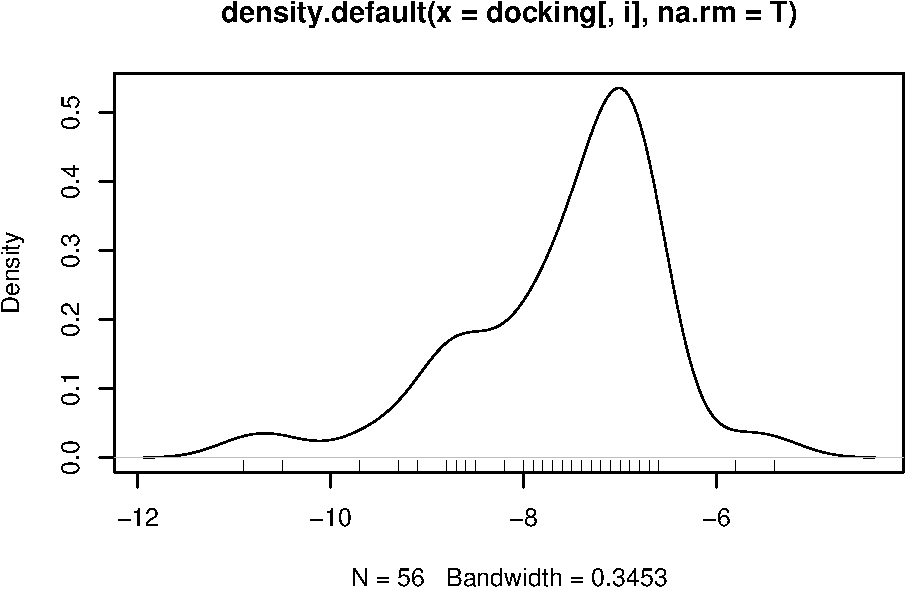
\includegraphics{chap4_files/figure-latex/johan-2.pdf}

\texttt{\#\#\ debug\ en\ \textless{}text\textgreater{}\#4:\ rug(docking{[},\ i{]})\ \ \ \#\#\ debug\ en\ \textless{}text\textgreater{}\#4:\ browser()\ \ \ \#\#\ debug\ en\ \textless{}text\textgreater{}\#4:\ plot(density(docking{[},\ i{]},\ na.rm\ =\ T))}

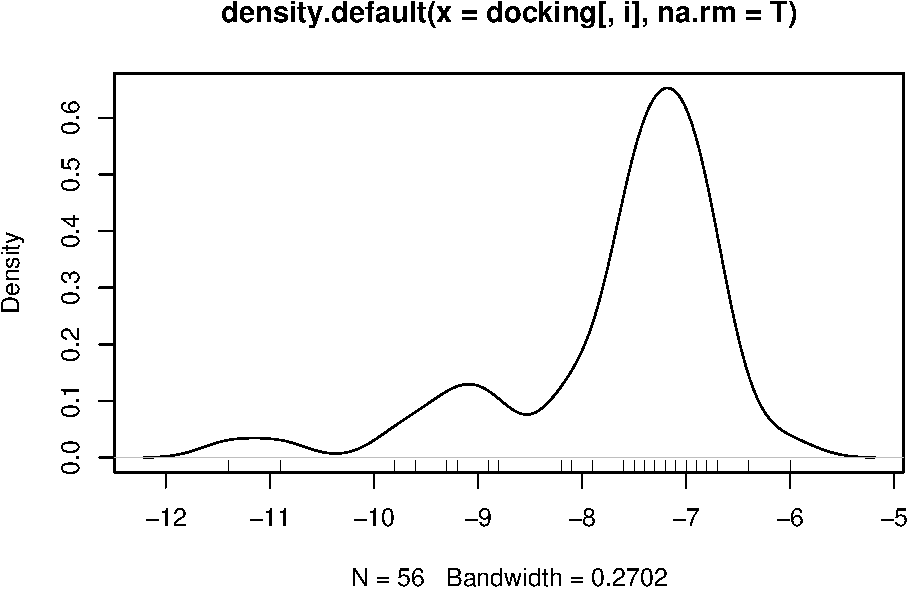
\includegraphics{chap4_files/figure-latex/johan-3.pdf}

\texttt{\#\#\ debug\ en\ \textless{}text\textgreater{}\#4:\ rug(docking{[},\ i{]})\ \ \ \#\#\ debug\ en\ \textless{}text\textgreater{}\#4:\ browser()\ \ \ \#\#\ debug\ en\ \textless{}text\textgreater{}\#4:\ plot(density(docking{[},\ i{]},\ na.rm\ =\ T))}

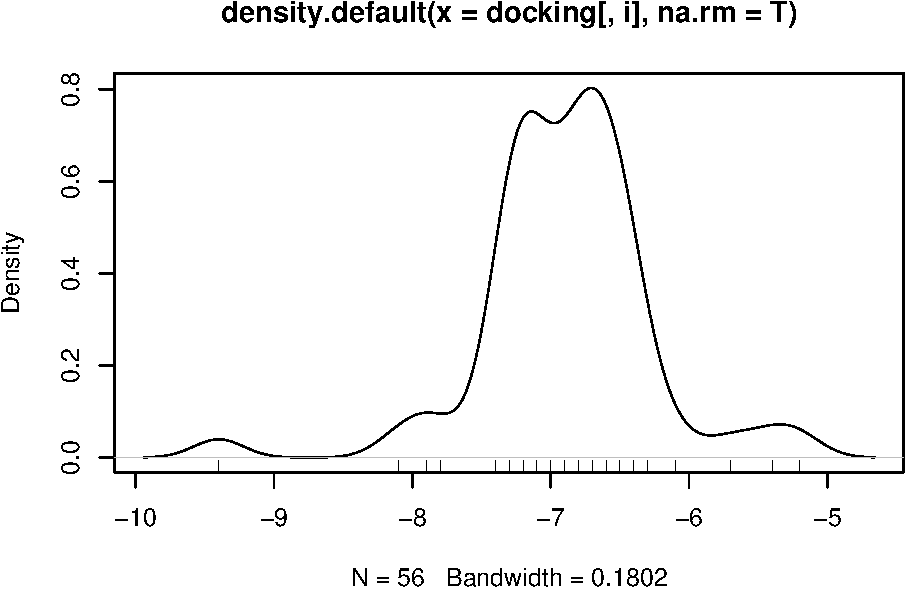
\includegraphics{chap4_files/figure-latex/johan-4.pdf}

\texttt{\#\#\ debug\ en\ \textless{}text\textgreater{}\#4:\ rug(docking{[},\ i{]})\ \ \ \#\#\ debug\ en\ \textless{}text\textgreater{}\#4:\ browser()\ \ \ \#\#\ debug\ en\ \textless{}text\textgreater{}\#4:\ plot(density(docking{[},\ i{]},\ na.rm\ =\ T))}

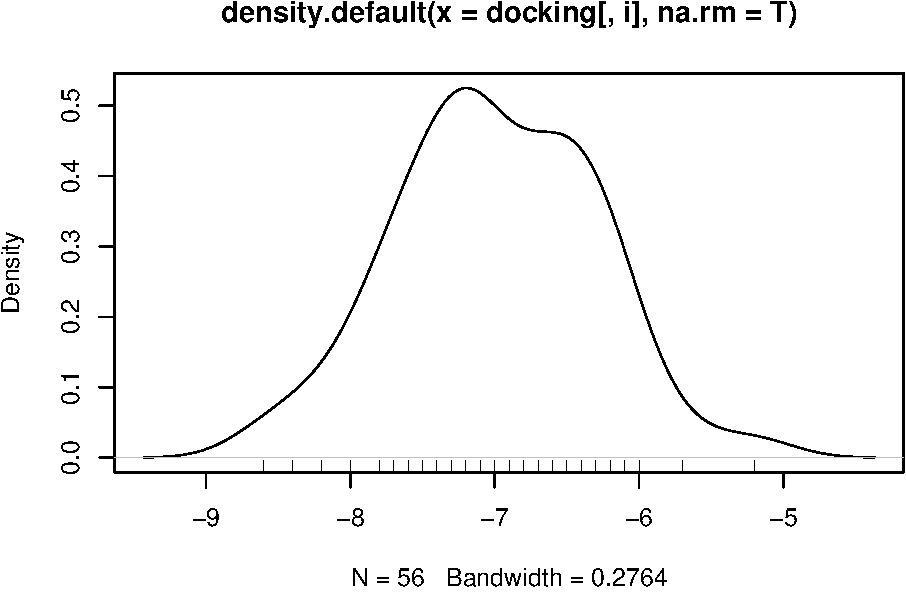
\includegraphics{chap4_files/figure-latex/johan-5.pdf}

\texttt{\#\#\ debug\ en\ \textless{}text\textgreater{}\#4:\ rug(docking{[},\ i{]})\ \ \ \#\#\ debug\ en\ \textless{}text\textgreater{}\#4:\ browser()\ \ \ \#\#\ debug\ en\ \textless{}text\textgreater{}\#4:\ plot(density(docking{[},\ i{]},\ na.rm\ =\ T))}

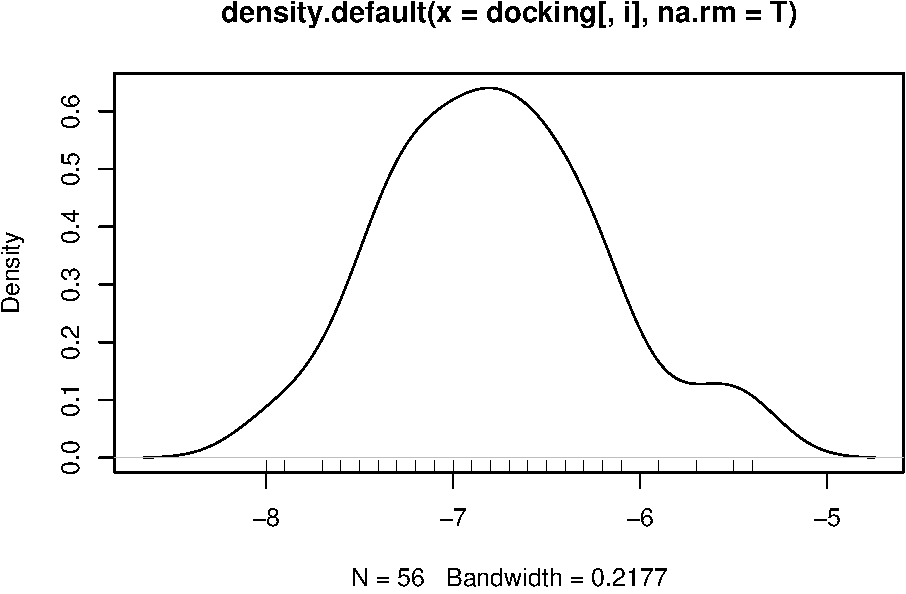
\includegraphics{chap4_files/figure-latex/johan-6.pdf}

\texttt{\#\#\ debug\ en\ \textless{}text\textgreater{}\#4:\ rug(docking{[},\ i{]})\ \ \ \#\#\ debug\ en\ \textless{}text\textgreater{}\#4:\ browser()\ \ \ \#\#\ debug\ en\ \textless{}text\textgreater{}\#4:\ plot(density(docking{[},\ i{]},\ na.rm\ =\ T))}

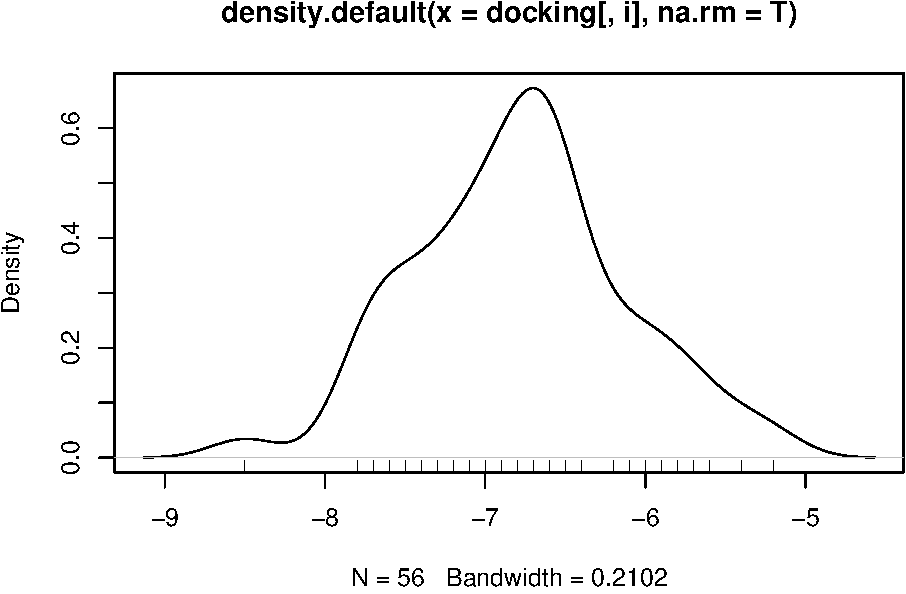
\includegraphics{chap4_files/figure-latex/johan-7.pdf}

\texttt{\#\#\ debug\ en\ \textless{}text\textgreater{}\#4:\ rug(docking{[},\ i{]})\ \ \ \#\#\ debug\ en\ \textless{}text\textgreater{}\#4:\ browser()\ \ \ \#\#\ debug\ en\ \textless{}text\textgreater{}\#4:\ plot(density(docking{[},\ i{]},\ na.rm\ =\ T))}

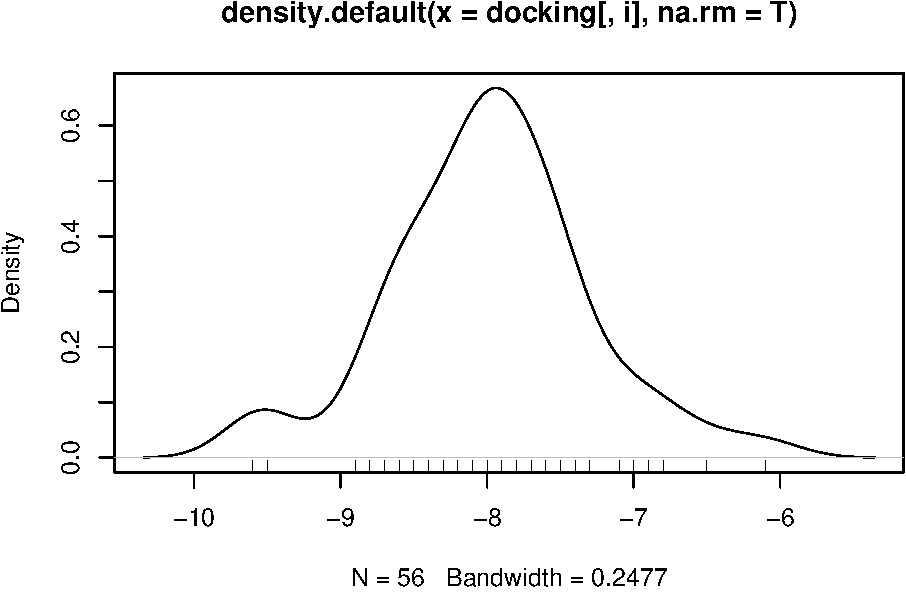
\includegraphics{chap4_files/figure-latex/johan-8.pdf}

\texttt{\#\#\ debug\ en\ \textless{}text\textgreater{}\#4:\ rug(docking{[},\ i{]})\ \ \ \#\#\ debug\ en\ \textless{}text\textgreater{}\#4:\ browser()\ \ \ \#\#\ debug\ en\ \textless{}text\textgreater{}\#4:\ plot(density(docking{[},\ i{]},\ na.rm\ =\ T))}

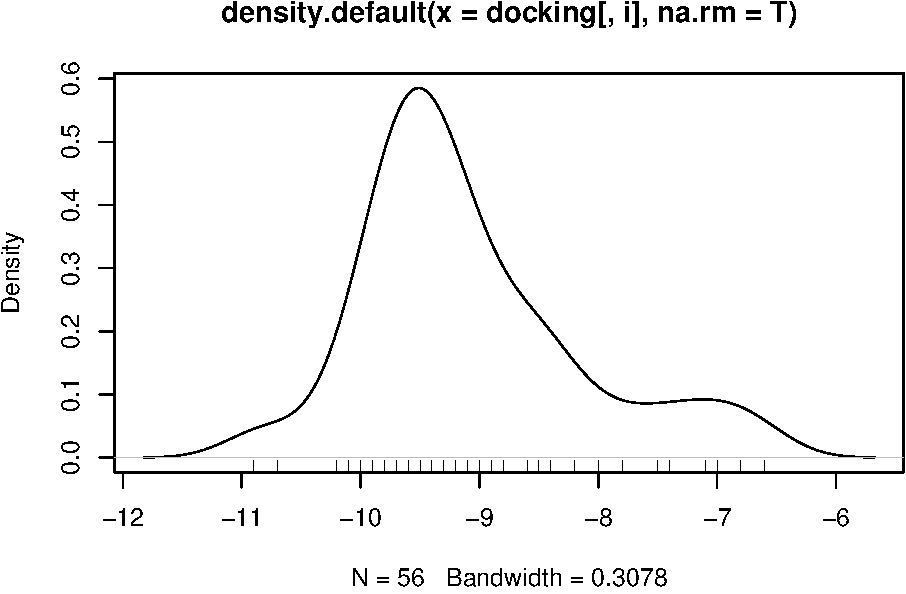
\includegraphics{chap4_files/figure-latex/johan-9.pdf}

\texttt{\#\#\ debug\ en\ \textless{}text\textgreater{}\#4:\ rug(docking{[},\ i{]})\ \ \ \#\#\ debug\ en\ \textless{}text\textgreater{}\#4:\ browser()\ \ \ \#\#\ debug\ en\ \textless{}text\textgreater{}\#4:\ plot(density(docking{[},\ i{]},\ na.rm\ =\ T))}

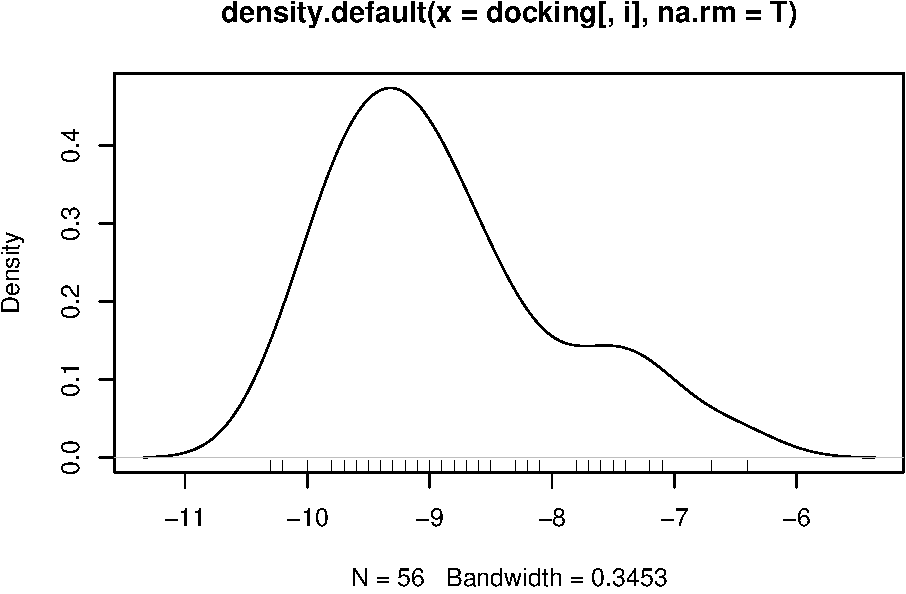
\includegraphics{chap4_files/figure-latex/johan-10.pdf}

\texttt{\#\#\ debug\ en\ \textless{}text\textgreater{}\#4:\ rug(docking{[},\ i{]})\ \ \ \#\#\ debug\ en\ \textless{}text\textgreater{}\#4:\ browser()\ \ \ \#\#\ debug\ en\ \textless{}text\textgreater{}\#4:\ plot(density(docking{[},\ i{]},\ na.rm\ =\ T))}

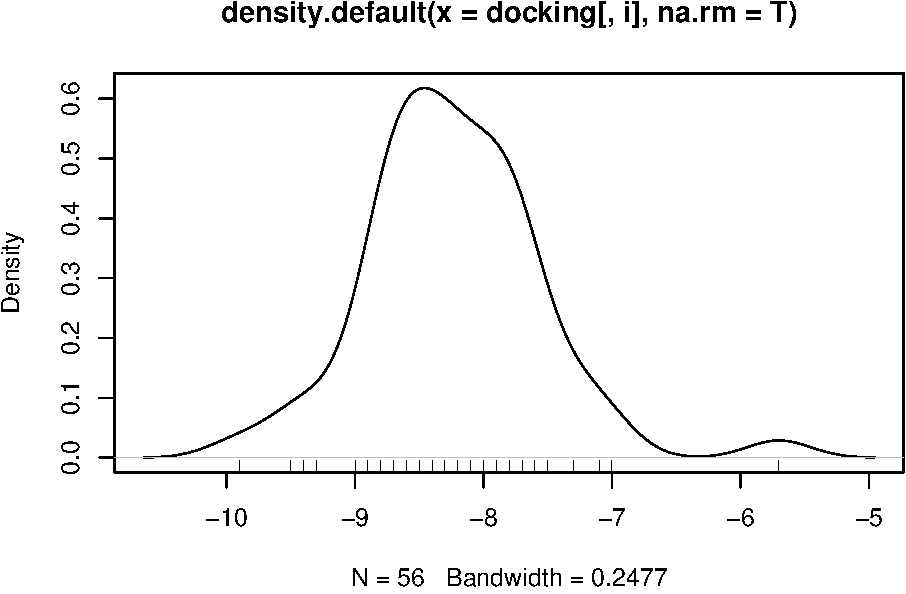
\includegraphics{chap4_files/figure-latex/johan-11.pdf}

\texttt{\#\#\ debug\ en\ \textless{}text\textgreater{}\#4:\ rug(docking{[},\ i{]})\ \ \ \#\#\ debug\ en\ \textless{}text\textgreater{}\#4:\ browser()\ \ \ \#\#\ debug\ en\ \textless{}text\textgreater{}\#4:\ plot(density(docking{[},\ i{]},\ na.rm\ =\ T))}

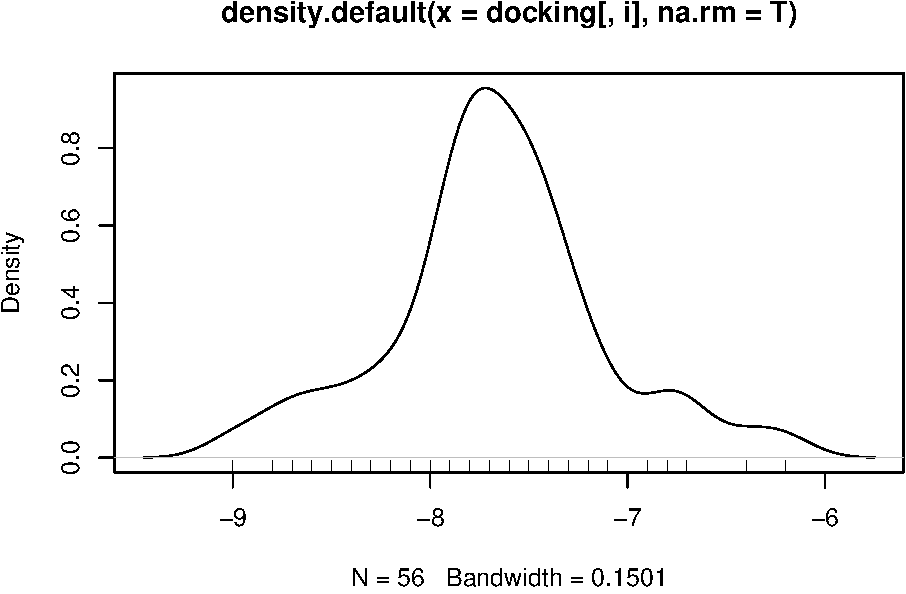
\includegraphics{chap4_files/figure-latex/johan-12.pdf}

\texttt{\#\#\ debug\ en\ \textless{}text\textgreater{}\#4:\ rug(docking{[},\ i{]})\ \ \ \#\#\ debug\ en\ \textless{}text\textgreater{}\#4:\ browser()\ \ \ \#\#\ debug\ en\ \textless{}text\textgreater{}\#4:\ plot(density(docking{[},\ i{]},\ na.rm\ =\ T))}

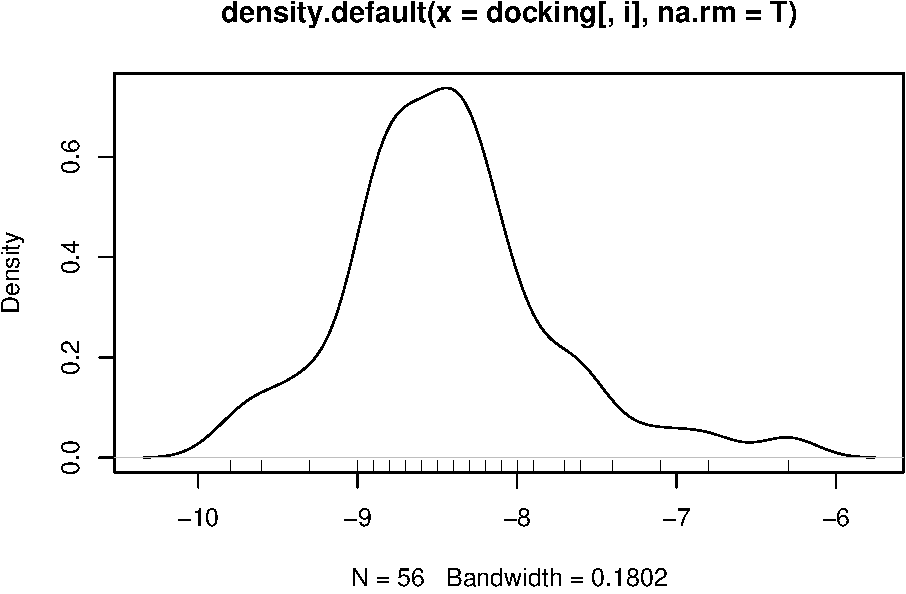
\includegraphics{chap4_files/figure-latex/johan-13.pdf}

\texttt{\#\#\ debug\ en\ \textless{}text\textgreater{}\#4:\ rug(docking{[},\ i{]})\ \ \ \#\#\ debug\ en\ \textless{}text\textgreater{}\#4:\ browser()\ \ \ \#\#\ debug\ en\ \textless{}text\textgreater{}\#4:\ plot(density(docking{[},\ i{]},\ na.rm\ =\ T))}

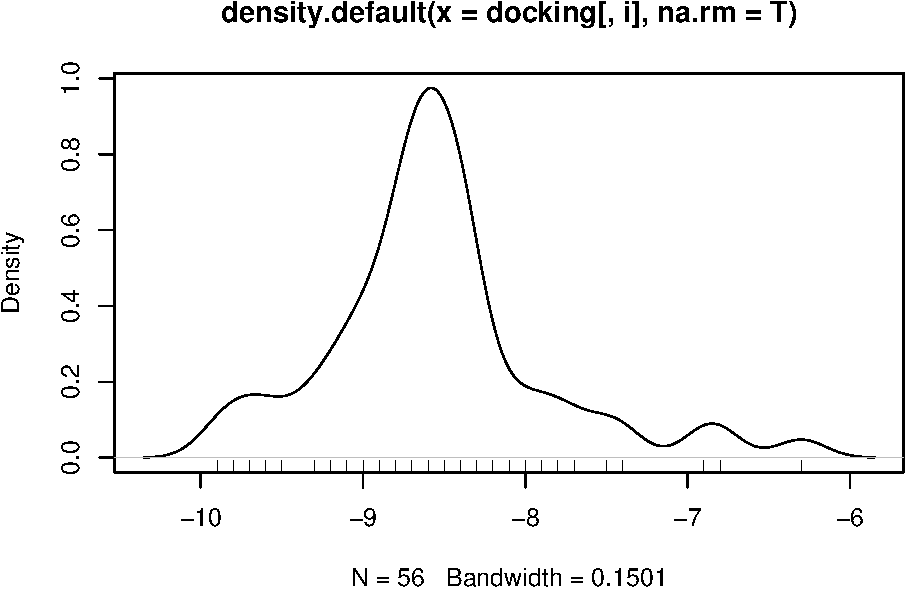
\includegraphics{chap4_files/figure-latex/johan-14.pdf}

\texttt{\#\#\ debug\ en\ \textless{}text\textgreater{}\#4:\ rug(docking{[},\ i{]})\ \ \ \#\#\ debug\ en\ \textless{}text\textgreater{}\#4:\ browser()\ \ \ \#\#\ debug\ en\ \textless{}text\textgreater{}\#4:\ plot(density(docking{[},\ i{]},\ na.rm\ =\ T))}

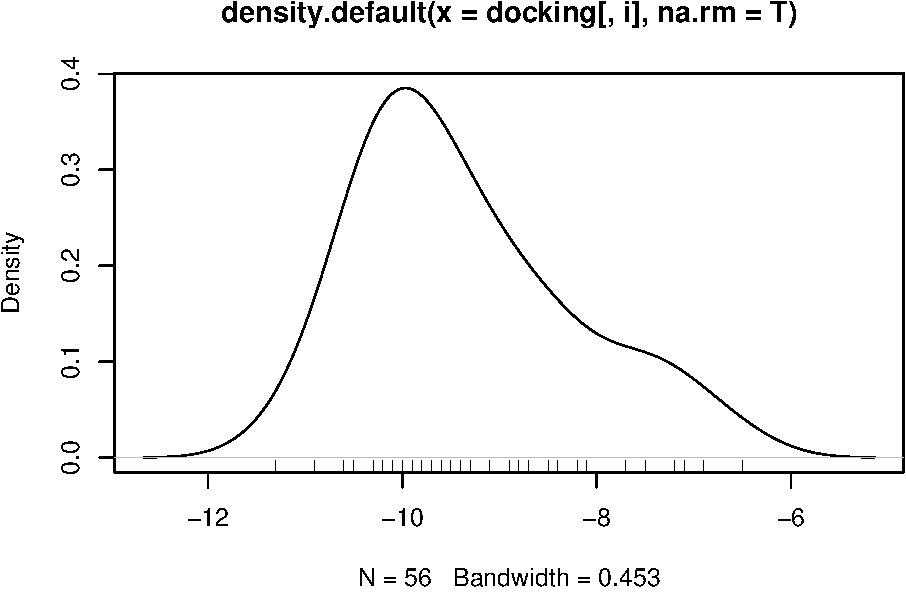
\includegraphics{chap4_files/figure-latex/johan-15.pdf}

\texttt{\#\#\ debug\ en\ \textless{}text\textgreater{}\#4:\ rug(docking{[},\ i{]})\ \ \ \#\#\ debug\ en\ \textless{}text\textgreater{}\#4:\ browser()\ \ \ \#\#\ debug\ en\ \textless{}text\textgreater{}\#4:\ plot(density(docking{[},\ i{]},\ na.rm\ =\ T))}

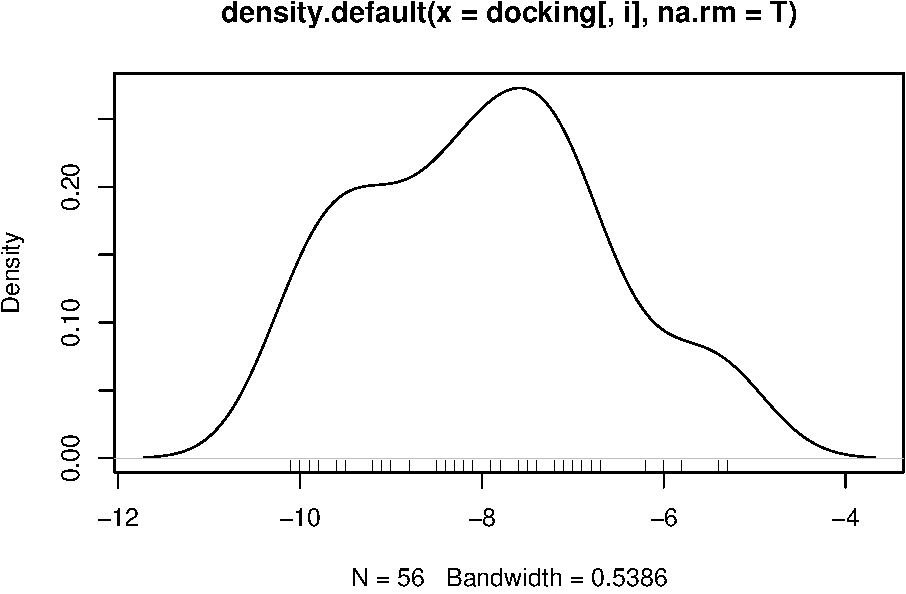
\includegraphics{chap4_files/figure-latex/johan-16.pdf}

\texttt{\#\#\ debug\ en\ \textless{}text\textgreater{}\#4:\ rug(docking{[},\ i{]})\ \ \ \#\#\ debug\ en\ \textless{}text\textgreater{}\#4:\ browser()\ \ \ \#\#\ debug\ en\ \textless{}text\textgreater{}\#4:\ plot(density(docking{[},\ i{]},\ na.rm\ =\ T))}

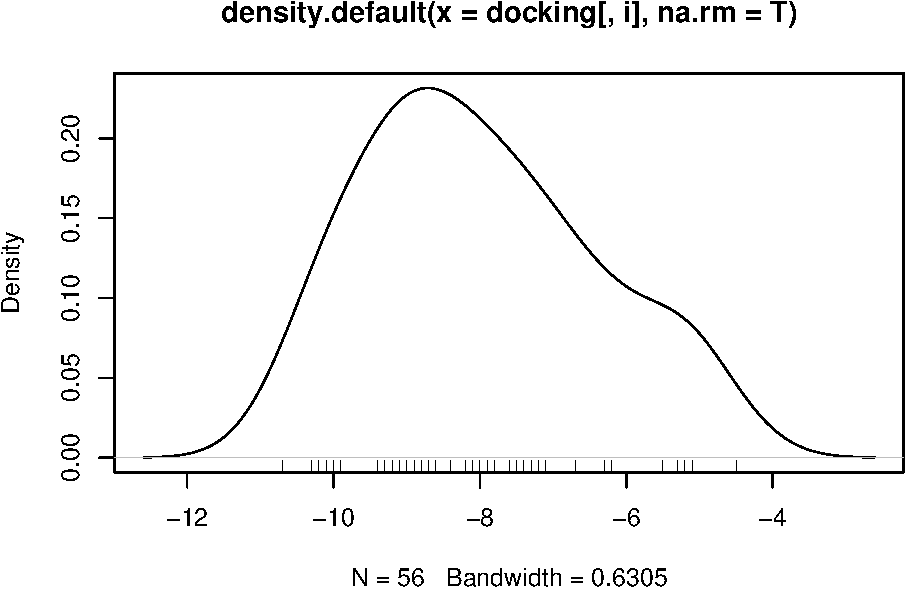
\includegraphics{chap4_files/figure-latex/johan-17.pdf}

\texttt{\#\#\ debug\ en\ \textless{}text\textgreater{}\#4:\ rug(docking{[},\ i{]})\ \ \ \#\#\ debug\ en\ \textless{}text\textgreater{}\#4:\ browser()\ \ \ \#\#\ debug\ en\ \textless{}text\textgreater{}\#4:\ plot(density(docking{[},\ i{]},\ na.rm\ =\ T))}

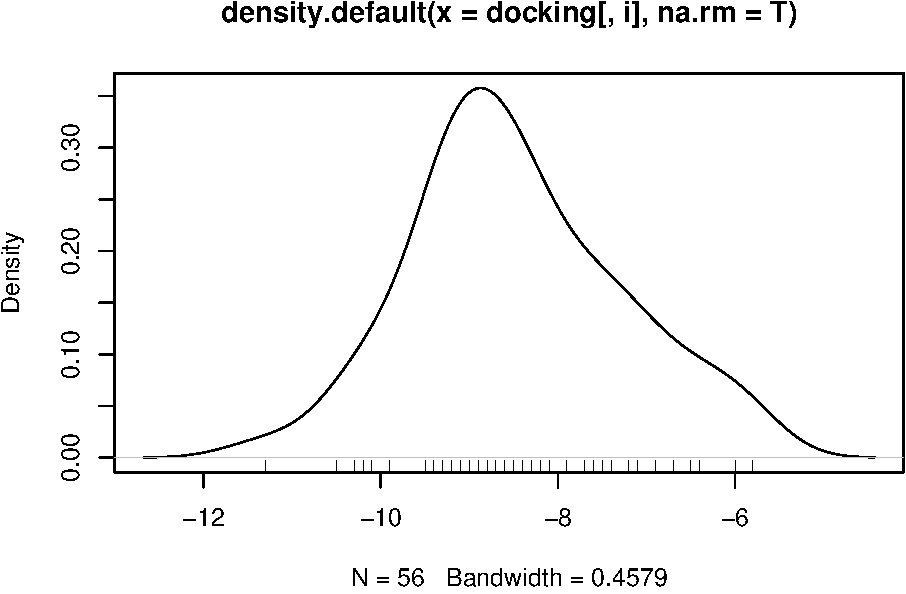
\includegraphics{chap4_files/figure-latex/johan-18.pdf}

\texttt{\#\#\ debug\ en\ \textless{}text\textgreater{}\#4:\ rug(docking{[},\ i{]})\ \ \ \#\#\ debug\ en\ \textless{}text\textgreater{}\#4:\ browser()\ \ \ \#\#\ debug\ en\ \textless{}text\textgreater{}\#4:\ plot(density(docking{[},\ i{]},\ na.rm\ =\ T))}

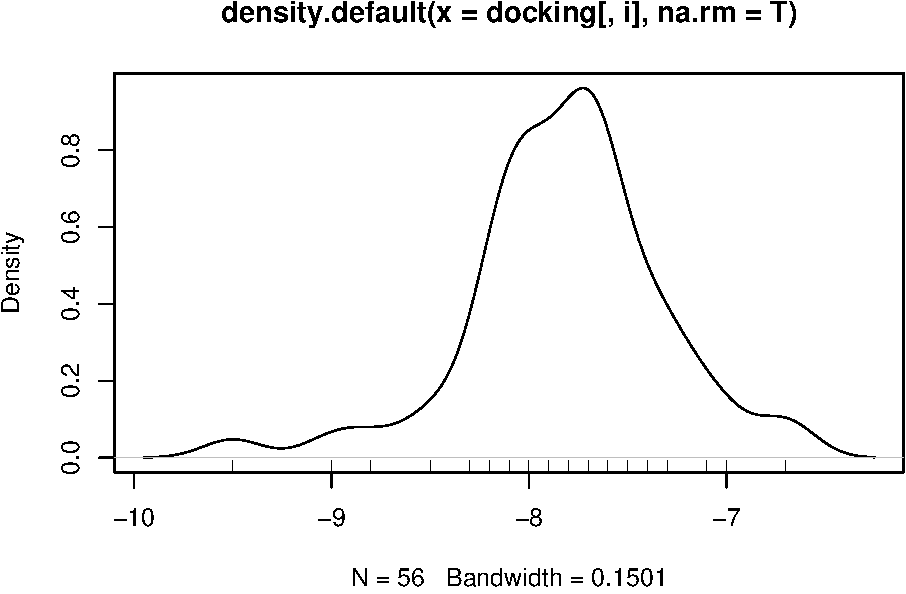
\includegraphics{chap4_files/figure-latex/johan-19.pdf}

\texttt{\#\#\ debug\ en\ \textless{}text\textgreater{}\#4:\ rug(docking{[},\ i{]})\ \ \ \#\#\ debug\ en\ \textless{}text\textgreater{}\#4:\ browser()\ \ \ \#\#\ debug\ en\ \textless{}text\textgreater{}\#4:\ plot(density(docking{[},\ i{]},\ na.rm\ =\ T))}

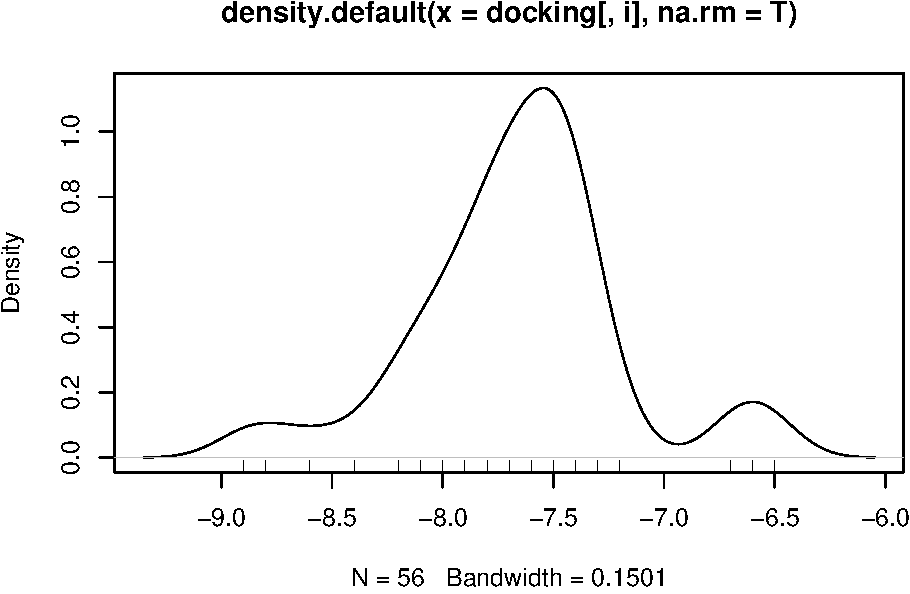
\includegraphics{chap4_files/figure-latex/johan-20.pdf}

\texttt{\#\#\ debug\ en\ \textless{}text\textgreater{}\#4:\ rug(docking{[},\ i{]})\ \ \ \#\#\ debug\ en\ \textless{}text\textgreater{}\#4:\ browser()}

\texttt{r\ \ \ plot(cor(docking{[}-c(5,12,13,38,51),-1{]}))}

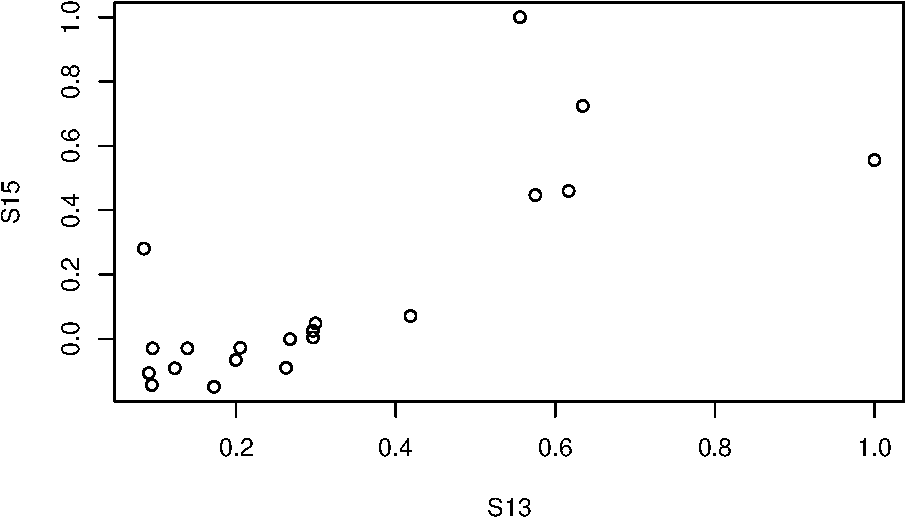
\includegraphics{chap4_files/figure-latex/johan-21.pdf}

\texttt{r\ \ \ \#\#\ Leer\ sobre\ la\ incertidumbre\ del\ 2\ y\ explicarla\ \ \ \ \ \#\#\ Y\ leer\ el\ paper\ de\ Julian\ y\ el\ de\ mauricio\ sobre\ reportes\ de\ docking}
---\textgreater{}

\begin{figure}[h!tbp]
\centering
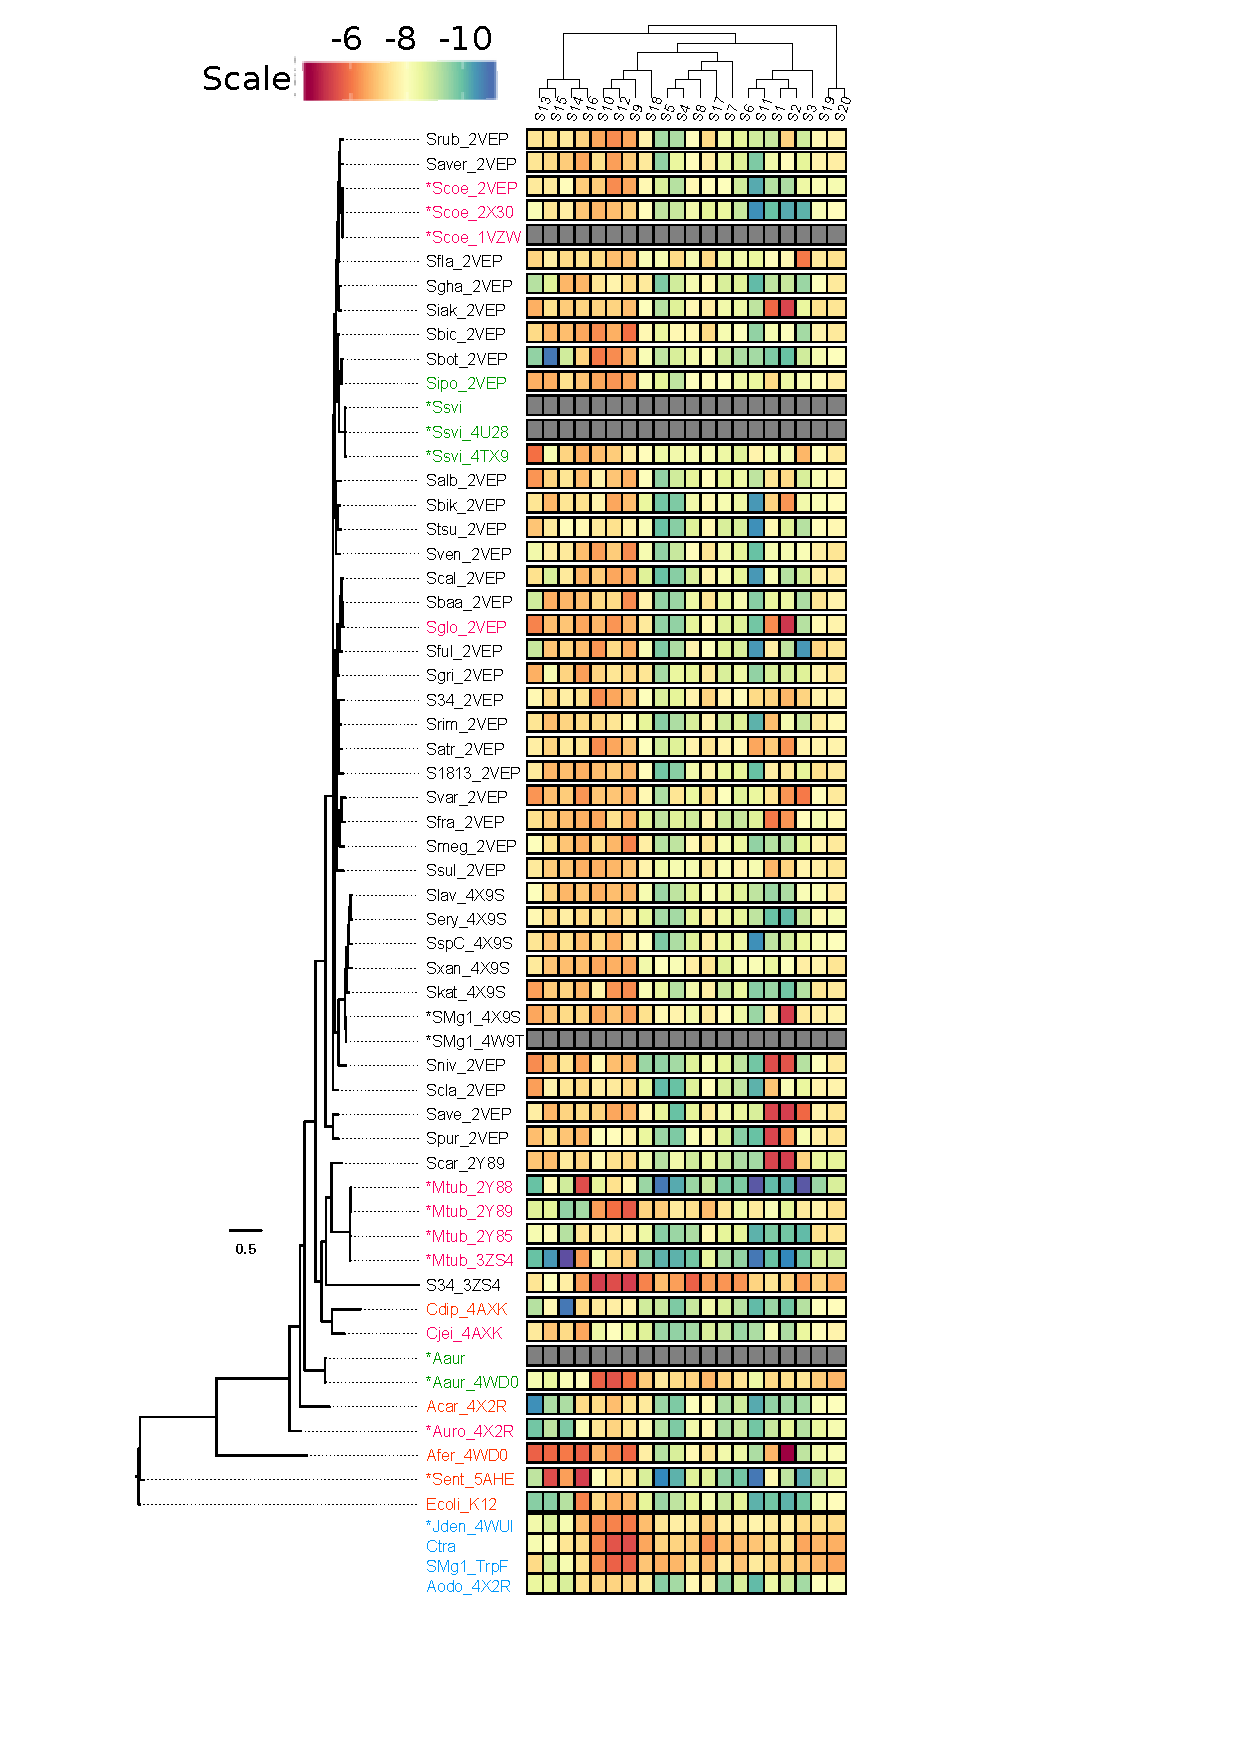
\includegraphics[angle = 0,scale = .7]{chapter4/Figura1_4.pdf}
\caption[Heatplot del docking de enzimas relacionadas a PriA vs posibles substratos]{\footnotesize{Heatplot del docking de enzimas relacionadas a PriA vs posibles substratos}}
\label{fig:HeatplodPriAdocking}
\end{figure}

\subsubsection{GTP es el sustrato por el que PriA muestra mayor
afinidad}\label{gtp-es-el-sustrato-por-el-que-pria-muestra-mayor-afinidad}

\begin{Shaded}
\begin{Highlighting}[]
\NormalTok{## boxplot de los sustratos}
\KeywordTok{ggplot}\NormalTok{(docking.m, }\KeywordTok{aes}\NormalTok{(}\DataTypeTok{x=}\NormalTok{variable, }\DataTypeTok{y=}\NormalTok{value)) +}\StringTok{ }\KeywordTok{labs}\NormalTok{(}\DataTypeTok{x =} \StringTok{"Substrates"}\NormalTok{, }\DataTypeTok{y =} \StringTok{"Affinity"}\NormalTok{,}\DataTypeTok{text =} \KeywordTok{element_text}\NormalTok{(}\DataTypeTok{size=}\DecValTok{12}\NormalTok{)) +}\StringTok{ }\KeywordTok{geom_boxplot}\NormalTok{()+}\KeywordTok{theme_bw}\NormalTok{()+}\KeywordTok{theme}\NormalTok{(}\DataTypeTok{plot.title =} \KeywordTok{element_text}\NormalTok{(}\DataTypeTok{size =} \DecValTok{14}\NormalTok{, }\DataTypeTok{face =} \StringTok{"bold"}\NormalTok{), }\DataTypeTok{text =} \KeywordTok{element_text}\NormalTok{(}\DataTypeTok{size =} \DecValTok{12}\NormalTok{), }\DataTypeTok{axis.title =} \KeywordTok{element_text}\NormalTok{(}\DataTypeTok{face=}\StringTok{"bold"}\NormalTok{), }\DataTypeTok{axis.text.x=}\KeywordTok{element_text}\NormalTok{(}\DataTypeTok{angle =} \DecValTok{90}\NormalTok{,}\DataTypeTok{size =} \DecValTok{6}\NormalTok{), }\DataTypeTok{legend.position =} \StringTok{"bottom"}\NormalTok{)}
\end{Highlighting}
\end{Shaded}

\begin{verbatim}
## Warning: Removed 100 rows containing non-finite values (stat_boxplot).
\end{verbatim}

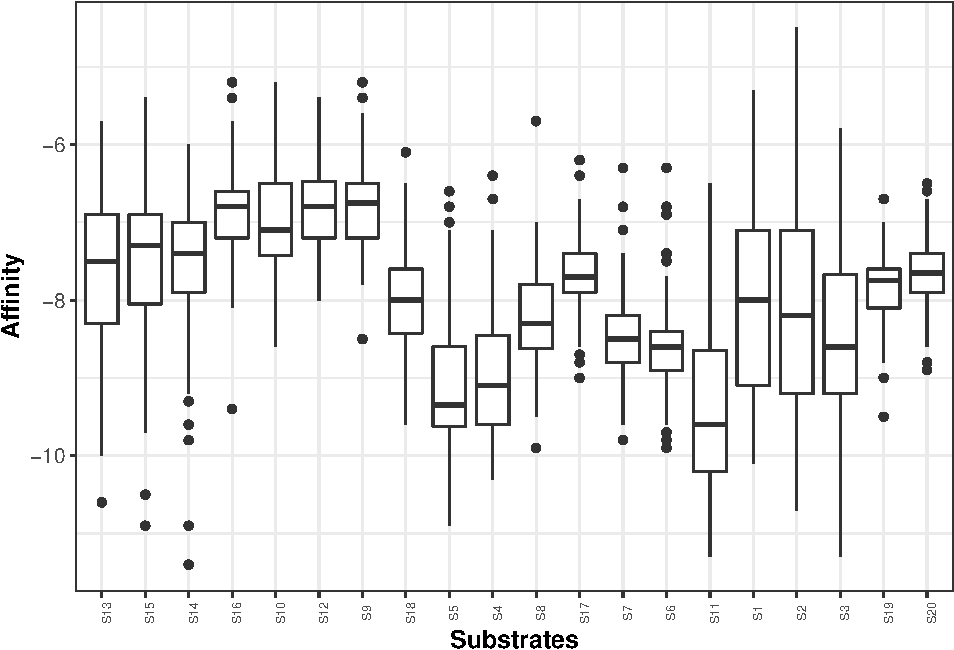
\includegraphics{chap4_files/figure-latex/substrateBox-1.pdf}

\clearpage  

\subsubsection{Dinámica molecular vs datos
experimentales}\label{dinamica-molecular-vs-datos-experimentales}

En las tablas \autoref{tab:PriAPRA} , \autoref{tab:PriAProFAR} se
muestra a detalle la comparación entre las dinámicas moleculares de PriA
respecto a PRA y ProFAR. Estos datos sugirieron que GTp es el sustrato
con mayor afinidad y por ello en la última sección se avanzó en la
realización de cinéticas enzimáticas con GTP.

Table: Actividad de PriA en S3 PRA \label{tab:PriAPRA}

\[ 
\resizebox{\columnwidth}{!}{%
\begin{tabular}{ l c r l l l l l}
\hline \\ [-1.5ex]
organism  &Family & $K_M    $     & $k_{cat}$        & $\frac{k_{cat}}{K_M}$ &Pre MD & Pos MD & Reference  \\ [1ex]
\hline \\ [-1.5ex]
Afer        &HisA   & $1.1\pm0.2$   &$  0.05\pm0.001    $& 0.045                  &-10.1    &-12.3       &Noda-García L et al 2015\\ [1ex]
Ecoli       &HisA   &$  1.6         $&$         4.9       $&3.1                   &-9.9   &-16       &Henn-Sax et al. (2002)\\ [1ex]
Sent        &HisA   &$  17.0 \pm0.1 $&$ 7.8 \pm 2.4   $&$4.5 × 10^5          $&-10.3  &-20.1     &Söderholm A et al (2015)\\ [1ex]
Aaur        &PriB   &$  2.1 \pm 0.5 $& $    1.8 \pm 0.2     $&0.9                   &-7.4   &              &verduzco-castro 2016\\ [1ex]
Sipo        &PriB   &$  3.8\pm0.2     $&$0.82\pm0.02        $&0.21                  &-8.2     &-14.7       &verduzco-castro 2016\\ [1ex]
SspC        &PriB   &$  11.4\pm3.4  $&$2.53\pm0.74      $&0.22                  &   -8.5    &-12.7     &verduzco-castro 2016\\ [1ex]
SMg1        &PriB   &$  13.2\pm3.4  $&$0.92\pm0.19      $&0.069                 &-8     &-15.2     &verduzco-castro 2016\\ [1ex]
Ssvi        &PriB   &$  3.9\pm0.89  $&$0.69\pm0.04      $&0.18                  &-8.2     &-16.7     &verduzco-castro 2016\\ [1ex]
Scoe        &PriA   &$  3.6\pm0.7     $&$ 1.3\pm0.2     $  &0.4                   &-8.4   &-15       &Noda-García et al (2010)\\ [1ex]
Sglob       &PriA   & $4.2\pm0.8     $ & $0.74\pm0.03    $   &0.18                  &-9.2     &-16.7       &verduzco-castro\\ [1ex]
Mtub 2Y85   &priA   &$  19  0.23      $&$0.012  -9.7          $&                      &       &          &Due et al 2011\\ [1ex]
Mtub 3ZS4   &priA   &$  ?                 $&$-9.9               $&                      &       &          &Due et al 2011 (To be published)\\ [1ex]
Auro        &priA   &$  4.0 \pm 0.9 $&$0.2 \pm 0.03   $&0.04                    &-9.2       &          &Vazquez-Juarez (2016)\\ [1ex]
Cjei        &PriA   &$  2.3 \pm 0.2 $&$0.9 \pm 0.08   $&0.39                    &-8.5       &          &Noda-García et al (2013)\\ [1ex]
Cdip        &subHisA&$  4.4 \pm 0.5 $&$2.6 \pm 0.3      $&0.59                  &-9.2       &          &Noda-García et al (2013)\\ [1ex]
SMg1 TrpF   &TrpF3  &   -                &-                &-                       &-6.9     &-9.6      &verduzco-castro 2016\\ [1ex]
Jden        &TrpF3  &   -                &-                &-          -7.2         &-9.4     &$16.8\pm3.3$&    Verduzco-Castro E et al  2016\\ [1ex]
Acar      &SubHisA& 0.02                     &                 &                        &       &          &            \\ [1ex]
Aodo        &SubTrpF&       -              &-                  &-                     &       &          &\\ [1ex]
\hline
\end{tabular}}
\label{tab:PriAPRA}  
%}
\]

\clearpage   La siguiente tabla es análoga a la anterior pero con el
sustrato ProFAR

Table: Actividad de PriA en S7 ProFAR \label{tab:PriAProFAR}

\[ 
\resizebox{\columnwidth}{!}{%
\centering 
\begin{tabular}{ l c r l l l l l}
\hline \\ [-1.5ex]
organism  &Family  &  $K_M$ & $k_{cat}$& $\frac{k{cat}}{K_M}$ &Pre MD &Pos MD &Reference  \\ [1ex]
\hline \\ [-1.5ex]
Afer      &HisA    &-            &-                &-          &-9.2    &-9        &Noda-García L et al. (2015)   \\ [1ex]
Ecoli     &HisA    &-            &-                &-          &-9      &-11.1     &Henn-Sax et al. (2002)\\ [1ex]
Sent      &HisA    &-            & -               &-          &-9.6    &-10.2     &Söderholm A et al (2015)\\ [1ex]
Aaur      &PriB    &$26.3\pm6.3$ & $0.37\pm 0.09$  & 0.014     &-7.1    &-         &verduzco-castro 2016\\ [1ex]
Sipo      &PriB    &$60.8\pm1.1$ &$8.25\pm0.4 $    &0.14       &-8      &-8.5      &verduzco-castro 2016 \\ [1ex]
SspC      &PriB    &$149.9\pm29$ &$1.4\pm0.12 $    &0.009      &-8.5    &-10.8     &verduzco-castro 2016\\ [1ex]
SMg1      &PriB    &$129.6\pm34$ &$0.29\pm0.04$    &0.0022     &-7.5    &-11       &verduzco-castro 2016\\ [1ex]
Ssvi      &PriB    &$24.5\pm4.0$ &$1.6\pm0.29 $    &0.067      &-8      &-9.7      &verduzco-castro 2016 \\ [1ex]
Scoe      &PriA    &$5.0\pm0.08$ &$3.4\pm0.09  $   &0.7        &-8      &-9.4      &Noda-García et al (2010)   \\ [1ex]
Sglob     &PriA    &$11\pm1.0$  &$3.8\pm0.2  $     &0.34       &-8.7    &-9.4      &verduzco-castro 2016  \\ [1ex]
Mtub2Y85  &priA    &21         &3.6         &0.17       &-8.6    &          &Due et al 2011                        \\ [1ex] 
Mtub3ZS4  &priA    &           &            &           &-9.3    &          &Due et al 2011 (To be published)      \\ [1ex] 
Auro      &priA    &$23 \pm 6.5 $  &$0.5\pm0.05 $&0.02       &-9.3    &          &Vazquez-Juarez (2016)                 \\ [1ex] 
Cjei      &PriA    &$5.1 \pm1.0$  &$1.6 \pm 0.16 $&0.31       &-9      &          &Noda-García et al (2013)              \\ [1ex]
Cdip      &subHisA &-          &-           &-          &-8.8    &          &Noda-García et al (2013)              \\ [1ex]
SMg1 TrpF &TrpF3   &$8.4\pm1.7$    &$10.5\pm2.4$    &1.25       &-7.6    &-9        &verduzco-castro     \\ [1ex] 
Jden      &TrpF3   &$16.8\pm3.3$   &$27\pm1.6$      &1.6        &-7.6    &-7.7      &verduzco-castro     \\ [1ex] 
Acar      &SubHisA &Na         &Na          &0.02       &Na      &Na        &Na                                    \\ [1ex] 
Aodo      &SubTrpF &-          &-           &-          &-       &Na        &Na                                    \\ [1ex]
\hline
\end{tabular}}
\label{tab:PriAProFAR}    
%}  
\]

\begin{table}[t]

\caption[Enzymes docking ]{\label{tab:docking_table_out}Enzymes docking \label{tab:docking}}
\centering
\resizebox{\linewidth}{!}{
\begin{tabular}{l|r|r|r|r|r|r|r|r|r|r|r|r|r|r|r|r|r|r|r|r}
\hline
Enzima & S13 & S15 & S14 & S16 & S10 & S12 & S9 & S18 & S5 & S4 & S8 & S17 & S7 & S6 & S11 & S1 & S2 & S3 & S19 & S20\\
\hline
Srub\_2VEP & -7.4 & -7.3 & -7.5 & -7.1 & -6.5 & -6.2 & -6.5 & -7.7 & -9.4 & -9.3 & -7.9 & -7.2 & -8.3 & -8.6 & -8.9 & -9.0 & -7.1 & -8.9 & -7.8 & -7.7\\
\hline
Saver\_2VEP & -7.4 & -7.2 & -7.0 & -6.5 & -7.3 & -6.4 & -7.0 & -7.5 & -9.6 & -8.5 & -7.9 & -7.6 & -8.4 & -8.7 & -9.8 & -8.3 & -7.9 & -8.6 & -7.7 & -7.6\\
\hline
Scoe\_2VEP & -7.5 & -7.5 & -7.9 & -7.0 & -7.0 & -6.2 & -6.5 & -7.8 & -8.8 & -9.2 & -7.8 & -7.9 & -8.0 & -8.9 & -10.3 & -9.2 & -9.3 & -8.4 & -8.1 & -8.2\\
\hline
Scoe\_2X30 & -8.1 & -7.4 & -7.6 & -6.9 & -6.7 & -6.8 & -7.1 & -7.9 & -9.1 & -9.0 & -8.3 & -8.6 & -8.5 & -9.0 & -10.6 & -10.0 & -10.3 & -10.2 & -8.1 & -7.9\\
\hline
Scoe\_1VZW & NA & NA & NA & NA & NA & NA & NA & NA & NA & NA & NA & NA & NA & NA & NA & NA & NA & NA & NA & NA\\
\hline
Sfla\_2VEP & -7.1 & -7.6 & -7.2 & -7.3 & -7.2 & -6.8 & -6.9 & -8.1 & -8.2 & -7.2 & -8.2 & -7.2 & -8.4 & -8.3 & -8.5 & -7.9 & -7.8 & -6.0 & -7.5 & -7.3\\
\hline
Sgha\_2VEP & -9.2 & -8.7 & -6.7 & -6.7 & -7.4 & -7.7 & -7.2 & -7.5 & -9.8 & -8.9 & -8.2 & -7.8 & -8.8 & -8.7 & -10.1 & -9.1 & -9.0 & -9.5 & -8.0 & -7.5\\
\hline
Siak\_2VEP & -6.6 & -7.3 & -7.0 & -7.1 & -7.1 & -7.1 & -6.8 & -8.0 & -9.2 & -8.7 & -7.8 & -7.6 & -8.3 & -8.4 & -9.1 & -5.8 & -5.3 & -8.5 & -7.3 & -7.4\\
\hline
Sbic\_2VEP & -7.2 & -6.7 & -6.8 & -6.5 & -6.2 & -6.6 & -5.9 & -7.8 & -8.5 & -7.8 & -7.8 & -7.2 & -8.2 & -8.0 & -9.6 & -8.2 & -8.0 & -9.4 & -7.7 & -7.5\\
\hline
Sbot\_2VEP & -9.6 & -10.9 & -8.9 & -7.1 & -6.0 & -6.2 & -6.7 & -8.1 & -9.1 & -8.8 & -8.3 & -7.9 & -8.9 & -9.3 & -9.4 & -9.8 & -10.0 & -8.9 & -8.2 & -8.0\\
\hline
Sipo\_2VEP & -6.6 & -6.6 & -7.3 & -6.9 & -6.5 & -6.3 & -6.5 & -8.1 & -8.6 & -9.1 & -8.0 & -7.9 & -8.0 & -8.4 & -8.5 & -7.2 & -8.4 & -8.2 & -7.9 & -7.6\\
\hline
Ssvi & NA & NA & NA & NA & NA & NA & NA & NA & NA & NA & NA & NA & NA & NA & NA & NA & NA & NA & NA & NA\\
\hline
Ssvi\_4U28 & NA & NA & NA & NA & NA & NA & NA & NA & NA & NA & NA & NA & NA & NA & NA & NA & NA & NA & NA & NA\\
\hline
Ssvi\_4TX9 & -5.9 & -8.2 & -7.1 & -6.6 & -6.8 & -7.0 & -7.6 & -7.9 & -8.4 & -8.3 & -8.2 & -8.1 & -8.4 & -8.7 & -7.7 & -8.2 & -8.2 & -6.7 & -8.0 & -7.5\\
\hline
Salb\_2VEP & -6.3 & -7.1 & -7.4 & -6.8 & -7.7 & -6.9 & -6.6 & -8.0 & -9.6 & -8.9 & -8.6 & -7.9 & -8.6 & -8.4 & -9.1 & -7.4 & -7.2 & -8.8 & -8.1 & -7.8\\
\hline
Sbik\_2VEP & -7.4 & -6.7 & -7.4 & -7.3 & -7.7 & -6.5 & -6.8 & -8.5 & -9.9 & -9.8 & -8.3 & -7.8 & -8.2 & -8.4 & -10.5 & -7.1 & -6.3 & -8.3 & -8.1 & -7.9\\
\hline
Stsu\_2VEP & -6.9 & -7.5 & -7.9 & -7.8 & -7.5 & -7.3 & -7.7 & -8.1 & -10.0 & -9.7 & -8.7 & -7.8 & -8.8 & -8.8 & -10.6 & -7.8 & -8.7 & -9.2 & -7.9 & -7.8\\
\hline
Sven\_2VEP & -8.3 & -7.6 & -7.5 & -6.8 & -6.4 & -7.0 & -6.2 & -8.2 & -9.6 & -9.0 & -7.9 & -7.4 & -8.3 & -8.6 & -10.0 & -8.2 & -8.2 & -8.1 & -7.6 & -7.4\\
\hline
Scal\_2VEP & -7.3 & -8.8 & -7.5 & -6.7 & -7.0 & -6.5 & -6.5 & -8.7 & -10.0 & -9.7 & -8.8 & -7.7 & -8.2 & -8.6 & -10.5 & -8.1 & -9.2 & -8.9 & -7.6 & -7.6\\
\hline
Sbaa\_2VEP & -8.9 & -6.6 & -6.7 & -6.8 & -7.2 & -7.2 & -6.2 & -7.7 & -9.6 & -9.5 & -8.4 & -7.4 & -8.5 & -8.2 & -9.7 & -8.5 & -8.4 & -9.3 & -7.4 & -7.7\\
\hline
Sglo\_2VEP & -6.1 & -6.8 & -6.9 & -6.5 & -6.7 & -6.3 & -6.7 & -7.5 & -9.6 & -9.6 & -8.6 & -7.8 & -8.7 & -8.7 & -9.9 & -6.2 & -5.1 & -9.2 & -7.8 & -7.7\\
\hline
Sful\_2VEP & -9.0 & -6.9 & -7.1 & -6.8 & -6.3 & -7.2 & -6.6 & -8.1 & -9.8 & -9.3 & -7.7 & -8.0 & -8.7 & -8.8 & -10.5 & -7.6 & -9.1 & -10.5 & -7.1 & -7.4\\
\hline
Sgri\_2VEP & -6.6 & -8.2 & -7.1 & -6.4 & -7.1 & -7.4 & -7.1 & -7.4 & -9.4 & -8.5 & -8.6 & -7.5 & -8.8 & -8.4 & -9.6 & -8.8 & -8.8 & -8.7 & -7.7 & -7.5\\
\hline
S34\_2VEP & -7.8 & -7.2 & -7.6 & -7.3 & -6.2 & -6.5 & -6.9 & -8.0 & -8.8 & -8.6 & -7.7 & -7.1 & -7.7 & -7.9 & -7.2 & -7.1 & -6.7 & -7.1 & -7.7 & -7.7\\
\hline
Srim\_2VEP & -7.4 & -6.8 & -7.1 & -7.2 & -7.2 & -7.4 & -7.8 & -8.6 & -9.7 & -9.3 & -8.8 & -7.7 & -8.9 & -8.7 & -10.2 & -6.8 & -8.2 & -9.0 & -7.5 & -7.8\\
\hline
Satr\_2VEP & -7.6 & -7.1 & -7.5 & -7.4 & -6.2 & -6.5 & -6.9 & -8.0 & -8.9 & -8.7 & -7.7 & -7.4 & -7.7 & -7.8 & -6.5 & -7.0 & -6.3 & -7.7 & -7.7 & -7.7\\
\hline
S1813\_2VEP & -7.5 & -6.7 & -6.8 & -6.6 & -6.8 & -7.0 & -6.7 & -7.9 & -9.9 & -9.7 & -8.3 & -7.7 & -8.5 & -8.6 & -10.0 & -7.6 & -7.5 & -8.6 & -7.3 & -7.5\\
\hline
Svar\_2VEP & -6.3 & -6.8 & -7.0 & -6.3 & -6.9 & -6.9 & -6.6 & -7.8 & -9.3 & -7.4 & -8.5 & -7.3 & -8.0 & -8.7 & -8.5 & -7.4 & -6.3 & -6.0 & -7.9 & -7.5\\
\hline
Sfra\_2VEP & -7.3 & -7.0 & -6.8 & -6.6 & -6.5 & -7.3 & -6.6 & -8.6 & -9.1 & -8.7 & -8.9 & -7.7 & -8.9 & -9.0 & -8.7 & -6.0 & -6.3 & -7.9 & -8.2 & -7.8\\
\hline
Smeg\_2VEP & -8.0 & -7.3 & -6.9 & -6.6 & -7.2 & -6.7 & -6.1 & -7.6 & -9.2 & -9.1 & -7.8 & -7.4 & -8.2 & -8.5 & -9.6 & -9.2 & -9.2 & -8.6 & -7.7 & -7.5\\
\hline
Ssul\_2VEP & -7.5 & -7.0 & -6.9 & -6.6 & -6.6 & -6.7 & -6.9 & -7.7 & -8.4 & -8.2 & -8.2 & -7.5 & -8.1 & -7.7 & -8.2 & -6.7 & -7.1 & -7.7 & -7.6 & -7.4\\
\hline
Slav\_4X9S & -8.0 & -7.1 & -6.7 & -6.9 & -6.6 & -6.8 & -6.7 & -8.2 & -9.5 & -9.1 & -8.6 & -8.0 & -8.4 & -8.7 & -9.1 & -9.5 & -9.3 & -8.1 & -8.1 & -7.6\\
\hline
Sery\_4X9S & -7.8 & -7.2 & -7.6 & -7.2 & -7.4 & -6.9 & -7.4 & -8.5 & -9.4 & -9.4 & -8.6 & -7.6 & -8.4 & -8.6 & -9.1 & -10.0 & -10.1 & -9.0 & -7.8 & -8.2\\
\hline
SspC\_4X9S & -7.4 & -6.9 & -7.3 & -6.8 & -7.3 & -6.6 & -7.5 & -8.0 & -9.8 & -9.3 & -8.7 & -7.6 & -8.5 & -8.4 & -10.6 & -9.1 & -8.9 & -8.5 & -8.1 & -8.0\\
\hline
Sxan\_4X9S & -7.5 & -6.9 & -6.8 & -6.8 & -6.5 & -6.6 & -6.5 & -8.3 & -8.0 & -8.1 & -7.6 & -7.4 & -8.7 & -8.1 & -8.1 & -8.5 & -8.0 & -7.6 & -7.7 & -7.4\\
\hline
Skat\_4X9S & -6.4 & -7.0 & -7.1 & -6.7 & -7.7 & -6.3 & -6.2 & -8.1 & -8.5 & -9.2 & -8.3 & -7.6 & -9.0 & -8.5 & -9.7 & -9.5 & -9.9 & -9.2 & -7.4 & -7.5\\
\hline
SMg1\_4X9S & -6.5 & -6.9 & -7.2 & -7.1 & -6.5 & -6.9 & -6.4 & -7.3 & -7.8 & -7.7 & -8.3 & -7.5 & -7.9 & -8.4 & -9.5 & -7.6 & -5.2 & -7.5 & -7.6 & -7.7\\
\hline
SMg1\_W9T & NA & NA & NA & NA & NA & NA & NA & NA & NA & NA & NA & NA & NA & NA & NA & NA & NA & NA & NA & NA\\
\hline
Sniv\_2VEP & -6.2 & -6.8 & -7.4 & -6.5 & -7.8 & -6.8 & -6.7 & -9.5 & -9.6 & -9.4 & -8.7 & -8.2 & -8.6 & -9.1 & -9.9 & -5.4 & -5.5 & -9.2 & -8.0 & -7.5\\
\hline
Scla\_2VEP & -6.4 & -7.7 & -7.4 & -7.2 & -7.6 & -7.5 & -7.2 & -8.5 & -10.1 & -10.0 & -8.7 & -7.9 & -8.8 & -9.1 & -10.2 & -6.9 & -8.1 & -8.5 & -7.7 & -7.7\\
\hline
Save\_2VEP & -7.6 & -6.7 & -7.1 & -7.2 & -7.1 & -6.5 & -6.6 & -7.8 & -8.6 & -10.0 & -8.6 & -7.5 & -8.3 & -8.5 & -8.8 & -5.3 & -5.2 & -5.8 & -7.7 & -7.4\\
\hline
Spur\_2vEP & -6.8 & -7.3 & -6.9 & -6.7 & -8.0 & -7.9 & -7.7 & -8.5 & -9.5 & -9.8 & -8.1 & -7.8 & -8.7 & -9.7 & -10.0 & -5.3 & -6.2 & -8.2 & -7.6 & -7.4\\
\hline
Scar\_2Y89 & -6.9 & -6.8 & -7.5 & -7.1 & -7.8 & -7.3 & -7.2 & -8.3 & -9.2 & -8.3 & -8.9 & -8.4 & -8.9 & -9.3 & -9.4 & -5.3 & -5.2 & -7.1 & -8.5 & -8.6\\
\hline
Mtub\_2Y88 & -10.0 & -7.8 & -8.9 & -5.4 & -8.6 & -7.3 & -7.8 & -9.5 & -10.9 & -10.3 & -9.5 & -9.0 & -9.8 & -9.8 & -11.3 & -10.1 & -10.2 & -11.3 & -9.5 & -8.8\\
\hline
Mtub\_2Y89 & -8.7 & -8.6 & -9.6 & -9.4 & -6.4 & -5.9 & -5.6 & -7.1 & -7.0 & -7.5 & -7.3 & -6.8 & -7.4 & -8.4 & -7.5 & -8.1 & -8.6 & -7.5 & -7.7 & -7.3\\
\hline
Mtub\_2Y85 & -8.2 & -7.9 & -9.2 & -7.4 & -7.6 & -7.5 & -7.6 & -8.4 & -9.7 & -9.5 & -9.3 & -7.8 & -8.6 & -8.6 & -10.2 & -9.8 & -9.9 & -10.1 & -7.3 & -7.4\\
\hline
Mtub\_3ZS4 & -10.0 & -10.5 & -11.4 & -6.4 & -8.2 & -7.2 & -7.0 & -9.6 & -10.2 & -10.2 & -9.9 & -8.5 & -9.3 & -9.6 & -10.9 & -10.0 & -10.7 & -9.9 & -8.8 & -8.9\\
\hline
S34\_3ZS4 & -7.4 & -8.0 & -7.6 & -6.4 & -5.2 & -5.4 & -5.2 & -6.1 & -6.8 & -6.4 & -5.7 & -6.4 & -6.3 & -6.3 & -7.1 & -7.4 & -7.1 & -6.4 & -7.1 & -6.6\\
\hline
Cdip\_4AXK & -9.2 & -7.8 & -10.9 & -7.2 & -7.5 & -7.6 & -7.7 & -8.9 & -9.0 & -9.8 & -9.0 & -8.3 & -8.8 & -9.2 & -10.1 & -9.5 & -9.9 & -9.2 & -8.0 & -7.9\\
\hline
Cjei\_4AXK & -7.5 & -6.9 & -7.2 & -6.5 & -8.4 & -8.0 & -8.5 & -8.7 & -9.5 & -9.6 & -9.4 & -8.8 & -9.0 & -9.5 & -9.3 & -8.1 & -9.3 & -8.5 & -7.9 & -7.7\\
\hline
Aaur & NA & NA & NA & NA & NA & NA & NA & NA & NA & NA & NA & NA & NA & NA & NA & NA & NA & NA & NA & NA\\
\hline
Aaur\_4WD0 & -8.2 & -8.5 & -8.1 & -7.9 & -5.7 & -5.5 & -5.9 & -7.0 & -7.5 & -7.2 & -7.1 & -6.7 & -7.1 & -7.4 & -8.4 & -7.2 & -7.3 & -7.4 & -7.0 & -6.7\\
\hline
Acar\_4X2R & -10.6 & -9.3 & -9.3 & -7.2 & -7.2 & -6.8 & -7.3 & -7.5 & -9.5 & -9.8 & -8.0 & -7.8 & -9.3 & -8.9 & -10.3 & -9.6 & -9.4 & -9.4 & -8.1 & -8.0\\
\hline
Auro\_4X2R & -9.9 & -9.1 & -9.8 & -8.1 & -7.4 & -7.1 & -7.4 & -7.8 & -9.2 & -9.8 & -8.3 & -7.8 & -9.3 & -9.0 & -9.9 & -9.0 & -8.6 & -9.2 & -8.5 & -8.2\\
\hline
Afer\_4WD0 & -5.7 & -5.8 & -6.0 & -5.7 & -6.7 & -6.2 & -5.8 & -7.6 & -9.2 & -8.8 & -7.8 & -7.4 & -8.3 & -8.4 & -9.3 & -6.7 & -4.5 & -9.1 & -8.3 & -8.1\\
\hline
Sent\_5AHE & -9.1 & -5.4 & -6.4 & -5.2 & -8.0 & -7.3 & -7.4 & -8.8 & -10.7 & -10.2 & -8.7 & -8.7 & -9.6 & -9.9 & -10.9 & -7.8 & -9.1 & -10.3 & -9.0 & -8.4\\
\hline
Ecoli\_K12 & -9.7 & -9.7 & -9.2 & -6.1 & -7.2 & -6.6 & -6.8 & -8.6 & -9.5 & -9.1 & -8.6 & -8.2 & -9.0 & -8.6 & -10.2 & -9.9 & -10.2 & -9.9 & -8.2 & -7.9\\
\hline
Jden\_4WUI & -8.3 & -8.8 & -8.2 & -6.8 & -6.2 & -6.1 & -6.0 & -6.8 & -7.4 & -7.6 & -7.5 & -6.9 & -7.6 & -7.5 & -7.7 & -7.5 & -7.6 & -7.2 & -7.3 & -7.2\\
\hline
Ctra & -8.2 & -8.0 & -7.4 & -7.2 & -6.1 & -5.5 & -5.4 & -6.5 & -7.1 & -7.1 & -7.0 & -6.2 & -6.8 & -6.8 & -6.9 & -7.2 & -7.4 & -6.5 & -6.7 & -6.6\\
\hline
SMg1\_trpF & -7.2 & -8.8 & -8.2 & -7.3 & -6.2 & -5.7 & -5.7 & -6.9 & -6.6 & -6.7 & -7.3 & -6.7 & -7.6 & -6.9 & -7.5 & -7.1 & -7.1 & -6.9 & -6.7 & -6.5\\
\hline
Aodo\_4X2R & -8.5 & -8.6 & -8.8 & -7.3 & -7.1 & -7.1 & -7.1 & -7.5 & -9.7 & -9.4 & -7.8 & -7.6 & -9.6 & -8.8 & -10.1 & -8.4 & -8.9 & -9.4 & -8.0 & -8.1\\
\hline
\end{tabular}}
\end{table}

Con actividad de FolE i.e activa para el compuesto V Adams et al (2014)

\clearpage  

\subsection{PriA en cinéticas enzimáticas no
tradicionales.}\label{pria-en-cineticas-enzimaticas-no-tradicionales.}

Además de la exploración genómica de PriA se realizaron
caracterizaciones experimentales. No se tuvo el tiempo ni la experiencia
para tener réplicas de los resultados descritos a continuación, sin
embargo pueden ser un buen comienzo para futuros estudiantes que deseen
retomarlos. Todos los protocolos fueron cuidadosamente descritos y se
encuentran en los anexos. Este capítulo se enfoca en el montaje de dos
experimentos. \emph{i)} Cinéticas de PriA en GTP . \emph{ii)} Medición
simultánea de la actividad de PriA sobre ProFAR y PRA.

Lo primero que se realizó fue la sobre expresión heteróloga de PriA y su
respectiva purificación para poder realizar \emph{in vitro} cinéticas
enzimáticas. Las enzimas fueron clonadas en cepas de \emph{E. coli} V68
se indujo sobre expresión y se purifico la proteína. Se corroboró el
éxito de esta actividad mediante un gel de proteína en la que puede
verse expresión en la barra correspondiente al tamaño de PriA
\autoref{fig:gel}.

\begin{figure}[h!tbp]
\centering
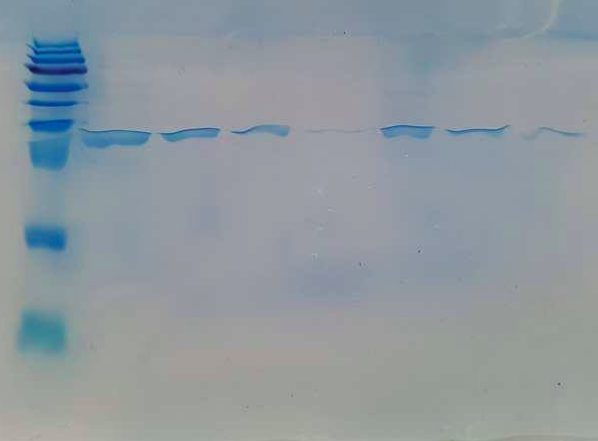
\includegraphics[angle = 0,scale = 0.6]{chapter4/Geles/PriAAbril30.png}
\caption[gel]{\footnotesize{Gel de proteína donde se muestra la banda correspondiente a PriA después de ser sobre-expresada y purificada}}
\label{fig:gel}
\end{figure}

Con la proteína purificada y almacenada a -80° en esferas de proteína
selladas con nitrógeno líquido como se describe en el anexo de los
procedimientos se procedió a realizar cinéticas enzimáticas.

\subsubsection{PriA puede tener actividad en
GTP}\label{pria-puede-tener-actividad-en-gtp}

La actividad fue medida fluorometricamente en placas de 96 (Nuc 96-Well
Optical Botto Plates) en un lector de placas TECAN infinite M1000 (con
exitación a 286 nm y emisión a 386 nm). Ensayos preliminares de
actividad se realizaron en una PriA activa respecto a los otros
substratos y proveniente de \emph{Streptomyces coelicolor} y en la
mutante inactiva D11A.

\begin{figure}[h!tbp]
\centering
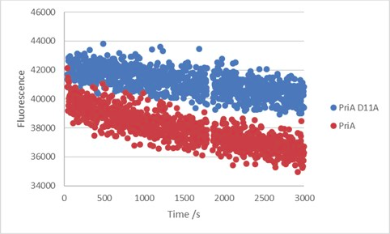
\includegraphics[angle = 0,scale = 0.8]{chapter4/MutantControl.png}
\caption[Scoe and non functional Scoe PriA acting on dGTP]{\footnotesize{}}
\label{fig:PriARutas1}
\end{figure}

\begin{figure}[h!tbp]
\centering
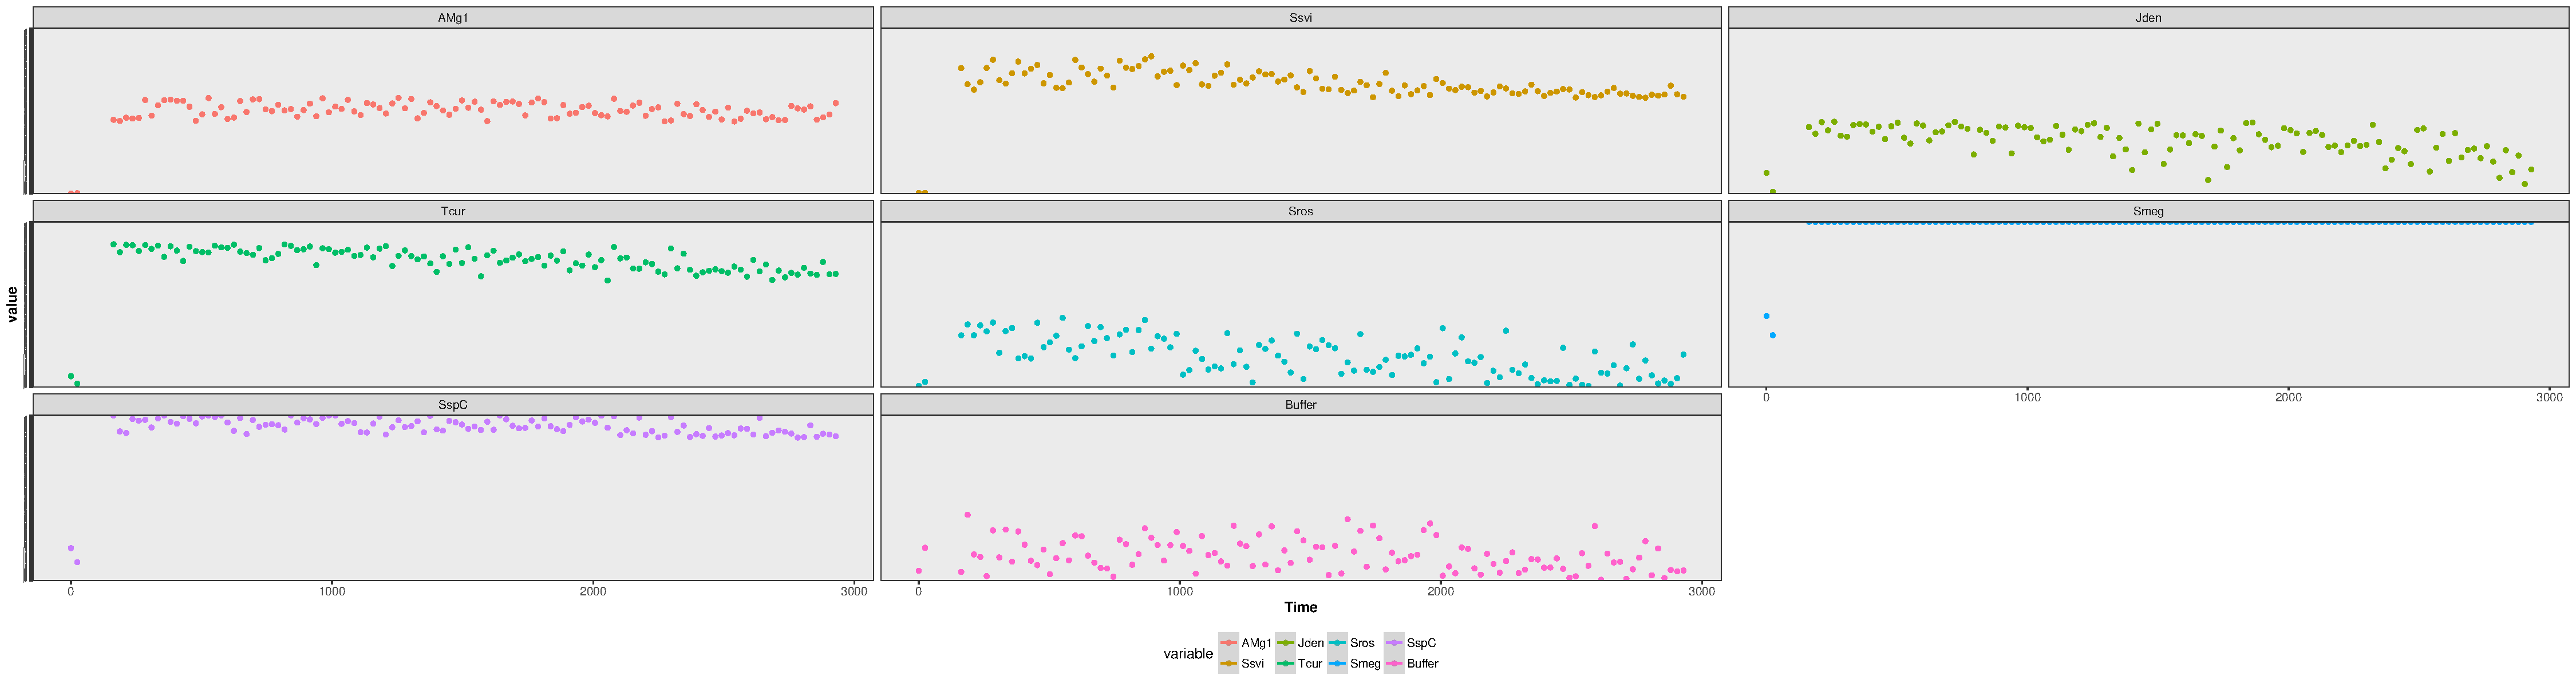
\includegraphics[angle = 0,scale = 0.6]{chapter4/GTPCinetica.pdf}
\caption[Scoe and non functional Scoe PriA acting on dGTP]{\footnotesize{}}
\label{fig:PriARutas2}
\end{figure}

\clearpage  

Entre las enzimas donde se aprecia actividad está \emph{Thermomonospora
curvata} que es una Actinobacteria termofílica de la familia
\emph{Thermomonosporaceae} y que puede ser encontrada encompostas ya que
participa en la degradación de celulosa {[}@chertkov\_complete\_2011{]}.
La trpF de \emph{Jonesia denitrificans} no mostró actividad.Esta
bacteria está clasificada como un organismo patogénico para animales, su
genoma fue originalmente aislado de sangre
{[}@pukall\_complete\_2009{]}.

\clearpage 

\subsubsection{Cinéticas simultáneas para PRA y
ProFAR}\label{cineticas-simultaneas-para-pra-y-profar}

En esta sección se tratpo de medir simultáneamente las actividades de
Pra y ProFAR.

\subsection{Cinéticas}\label{cineticas}

\begin{verbatim}
##   [1]    0.00   19.15   40.50   59.65   81.00  100.15  423.50  442.65
##   [9]  464.00  483.15  504.50  523.65  545.00  564.15  585.50  604.65
##  [17]  692.40  711.55  732.90  752.05  773.40  792.55  907.00  926.15
##  [25]  947.50  966.65  988.00 1007.15 1028.50 1047.65 1120.70 1139.85
##  [33] 1161.20 1180.35 1201.70 1220.85 1242.20 1261.35      NA      NA
##  [41] 1282.80 1301.95 1323.30 1342.45 1424.00 1443.15 1464.50 1483.65
##  [49] 1505.00 1524.15 1545.50 1564.65 1586.00 1605.15 1626.50 1645.65
##  [57] 1667.00 1686.15 1707.50 1726.65 1748.00 1767.15 1788.50 1807.65
##  [65] 1829.00 1848.15 1869.50 1888.65 1910.00 1929.15 1950.50 1969.65
##  [73] 1991.00 2010.15 2031.40 2050.55 2071.90 2091.05 2112.50 2131.65
##  [81] 2153.00 2172.15 2193.50 2212.65 2234.00 2253.15 2274.50 2293.65
##  [89] 2315.00 2334.15 2355.50 2374.65 2396.00 2415.15 2436.50 2455.65
##  [97] 2477.00 2496.15 2517.50 2536.65 2558.00 2577.15 2598.50 2617.65
## [105] 2639.00 2658.15 2679.50 2698.65 2720.00 2739.15 2760.50 2779.65
## [113] 2801.00 2820.15 2841.50 2860.65 2882.00 2901.15
\end{verbatim}

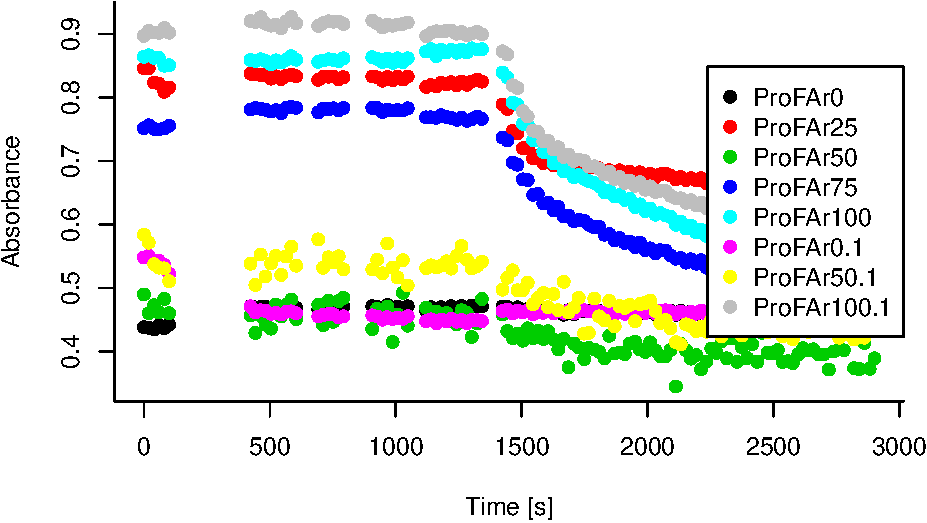
\includegraphics{chap4_files/figure-latex/Cinetics-1.pdf}
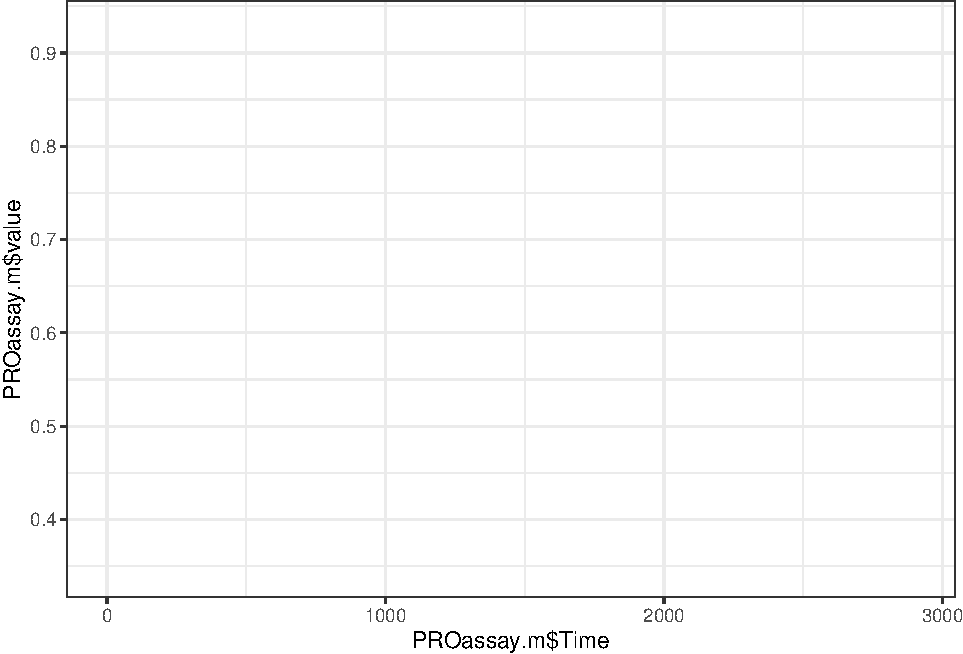
\includegraphics{chap4_files/figure-latex/Cinetics-2.pdf}
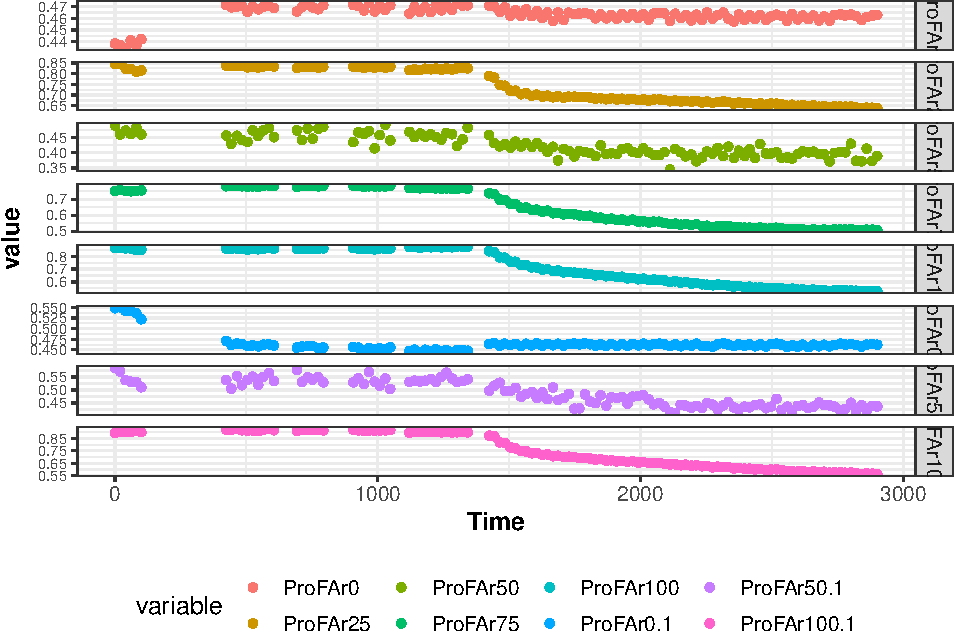
\includegraphics{chap4_files/figure-latex/Cinetics-3.pdf}

\begin{verbatim}
##   [1]    0.00   19.15   40.50   59.65   81.00  100.15  423.50  442.65
##   [9]  464.00  483.15  504.50  523.65  545.00  564.15  585.50  604.65
##  [17]  692.30  711.45  732.80  751.95  773.40  792.55  907.00  926.15
##  [25]  947.50  966.65  988.00 1007.15 1028.50 1047.65 1120.70 1139.85
##  [33] 1161.20 1180.35 1201.70 1220.85 1242.20 1261.35 1282.80 1301.95
##  [41] 1323.30 1342.45 1424.00 1443.15 1464.50 1483.65 1505.00 1524.15
##  [49] 1545.50 1564.65 1586.00 1605.15 1626.50 1645.65 1667.00 1686.15
##  [57] 1707.50 1726.65 1748.00 1767.15 1788.50 1807.65 1829.00 1848.15
##  [65] 1869.50 1888.65 1910.00 1929.15 1950.40 1969.55 1991.00 2010.15
##  [73] 2031.50 2050.65 2071.90 2091.05 2112.50 2131.65 2153.00 2172.15
##  [81] 2193.50 2212.65 2234.00 2253.15 2274.50 2293.65 2315.00 2334.15
##  [89] 2355.50 2374.65 2396.00 2415.15 2436.50 2455.65 2477.00 2496.15
##  [97] 2517.50 2536.65 2558.00 2577.15 2598.50 2617.65 2639.00 2658.15
## [105] 2679.50 2698.65 2720.00 2739.15 2760.50 2779.65 2801.00 2820.15
## [113] 2841.50 2860.65 2882.00 2901.15
\end{verbatim}

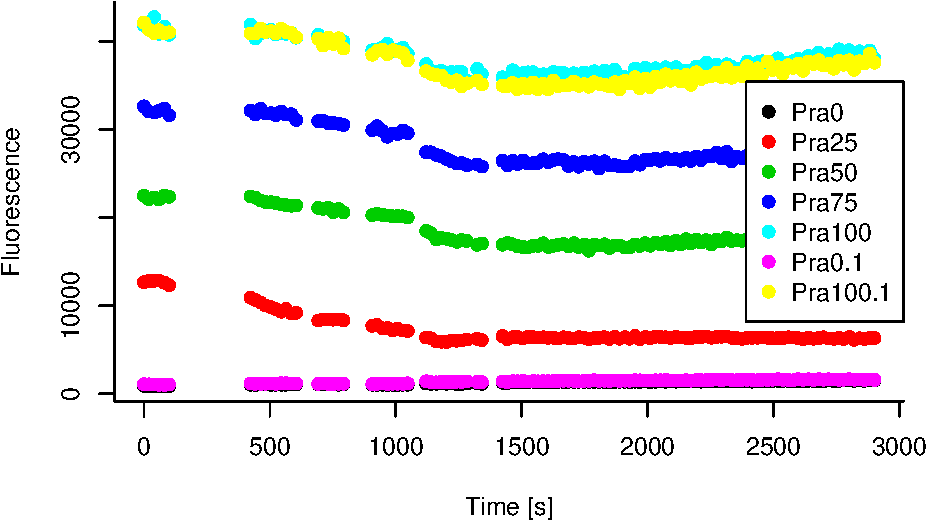
\includegraphics{chap4_files/figure-latex/Cinetics-4.pdf}
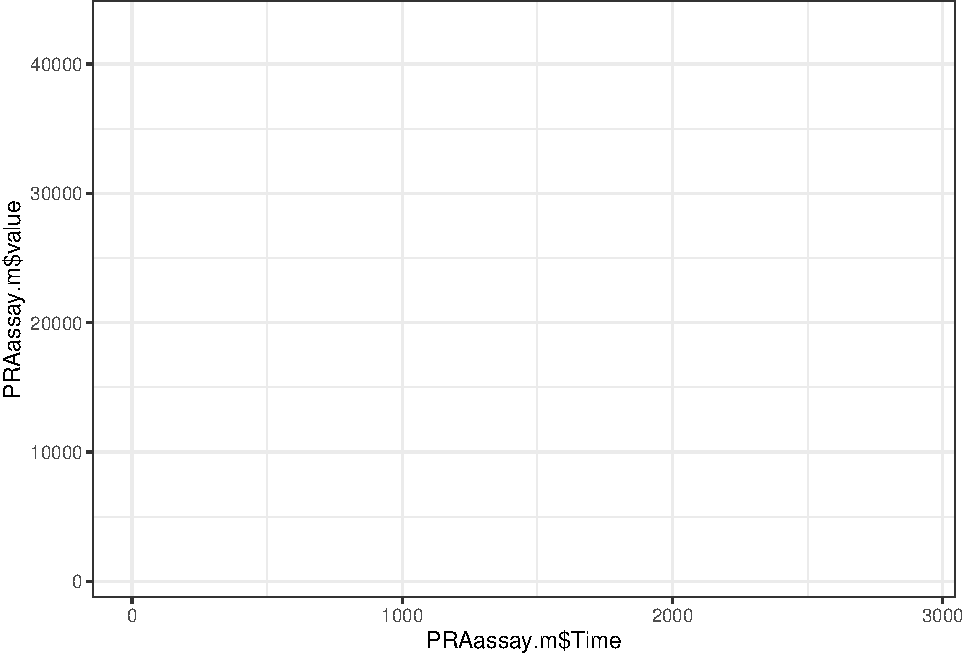
\includegraphics{chap4_files/figure-latex/Cinetics-5.pdf}
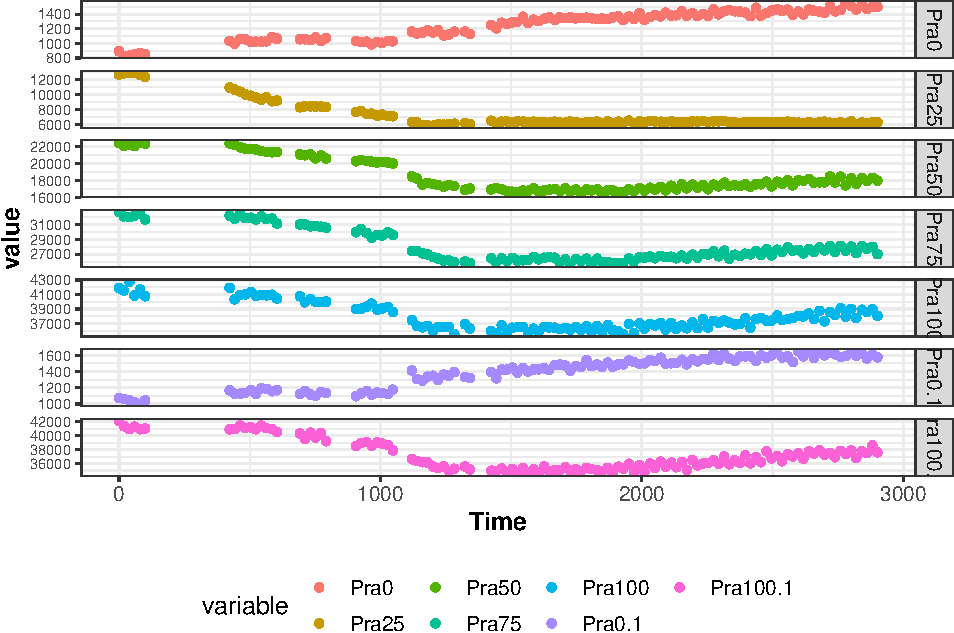
\includegraphics{chap4_files/figure-latex/Cinetics-6.pdf}

\subsection{Gráfico de pendientes}\label{grafico-de-pendientes}

\begin{verbatim}
## NULL
\end{verbatim}

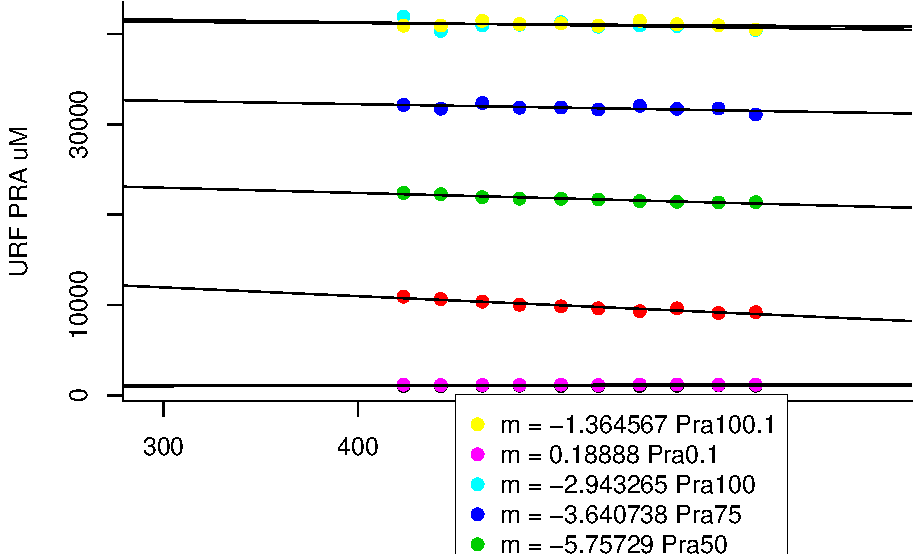
\includegraphics{chap4_files/figure-latex/slopes-1.pdf}

\begin{verbatim}
## [1]  0.196328 -9.695510 -5.757290 -3.640738 -2.943265  0.188880 -1.364567
\end{verbatim}

\begin{verbatim}
## [1]  0.196328 -9.695510 -5.757290 -3.640738 -2.943265  0.188880 -1.364567
\end{verbatim}

\begin{verbatim}
## [1]  1031 10920 22410 32161 41918  1168 40922
\end{verbatim}

\subsection{Interpolación con Michaelis
Menden}\label{interpolacion-con-michaelis-menden}

\begin{Shaded}
\begin{Highlighting}[]
\CommentTok{#sessionInfo()}
\end{Highlighting}
\end{Shaded}


\end{document}
